\chapter{Conception}
\fancyhead[R]{\textit{Conception}}
\renewcommand{\headrulewidth}{1pt}

\section{Introduction}
Dans ce chapitre, nous allons nous intéresser à la conception de notre système.
Le but est de définir et de mettre en place les choix d’architecture technique, 
et de compléter la description du système sous l’angle technique. Nous 
étendrons donc la représentation des diagrammes effectuée au niveau de 
l’analyse en y intégrant les aspects techniques les plus proches des 
préoccupations physiques.

\section{Modèle de domaine}
C’est le résultat d’une analyse du domaine. Il est considéré comme étant la 
première version du diagramme de classe. Ce modèle doit définir les classes 
qui modélisent les entités ou concepts présents dans le domaine (on utilise 
aussi le terme de métier) de l’application.

Il s’agit donc de produire un modèle des objets du monde réel dans un domaine 
donné. Ces entités ou concepts peuvent être identifiés directement à partir de 
la connaissance du domaine ou par des entretiens avec des experts du domaine. 
Il faut absolument utiliser le vocabulaire du métier pour nommer les classes et 
leurs attributs. Les classes du modèle de domaine ne doivent pas contenir des 
opérations, mais uniquement des attributs\cite{7}. Les étapes à suivre pour 
établir ce diagramme sont:

\begin{itemize}
    \item [\textbullet] Identifier les entités ou concepts du domaine.
    \item [\textbullet] Identifier et ajouter les associations et les attributs.
    \item [\textbullet] Organiser et simplifier le modèle en éliminant les 
        classes redondantes et en utilisant l'héritage.
    \item [\textbullet] Le cas échéant, structurer les classes en paquetage 
        selon les principes de cohérence et d'indépendance.
\end{itemize}

Comment identifier les concepts du domaine? Plutôt que de partir à l’aveugle 
et nous heurter à la taille du problème à résoudre, nous allons prendre les cas 
d’utilisation un par un et nous poser pour chacun la question suivante: quels 
sont les concepts métier qui participent à ce cas d’utilisation? En suivant 
cette méthode, nous avons sélectionné des cas d’utilisation différents afin 
d’avoir une vue globale sur les différentes entités qui composent le système 
sans répétition.

\subsection*{Modèle du domaine du cas d'utilisation « Se pointer »}
Pour marquer les horaires de travails d’un employé, nous avons besoin d’une 
entité employé, d'une empreinte pour l’identifier ainsi qu’une entité shift qui 
permet de sauvegarder ses pointages. 

\begin{figure}[h!]
    \centering
    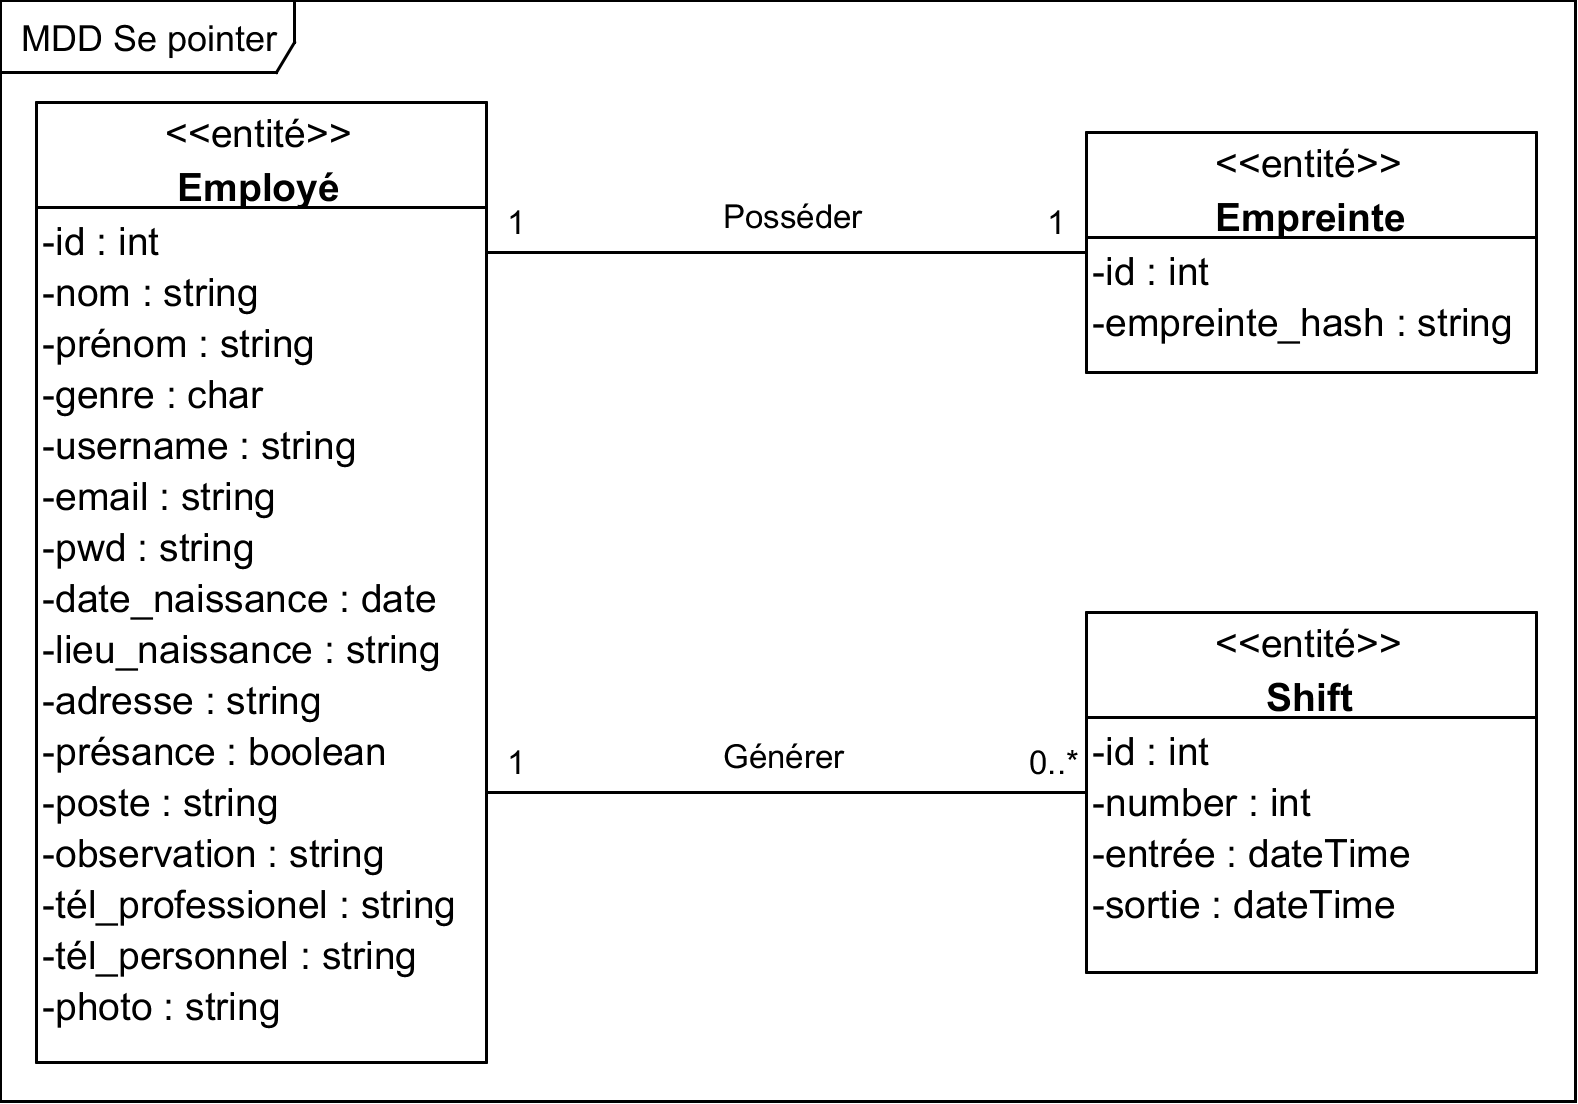
\includegraphics[scale=1.3]{images/MDD/MDD Se pointer.png}
    \caption{Modèle du domaine « Se pointer »}
    \label{fig12}
\end{figure}


\subsection*{Modèle du domaine du cas d'utilisation « Consulter ma fiche de pointage »}
Ce diagramme du modèle du domaine représente les entités concernées par le cas 
« Consulter ma fiche de pointage ». On peut distinguer deux entités: employé 
et Shift (qui représente une période de temps délimité par un temps d’entrée et 
un temps de sortie et la date de ces deux évènements).

\clearpage

\begin{figure}[h!]
    \centering
    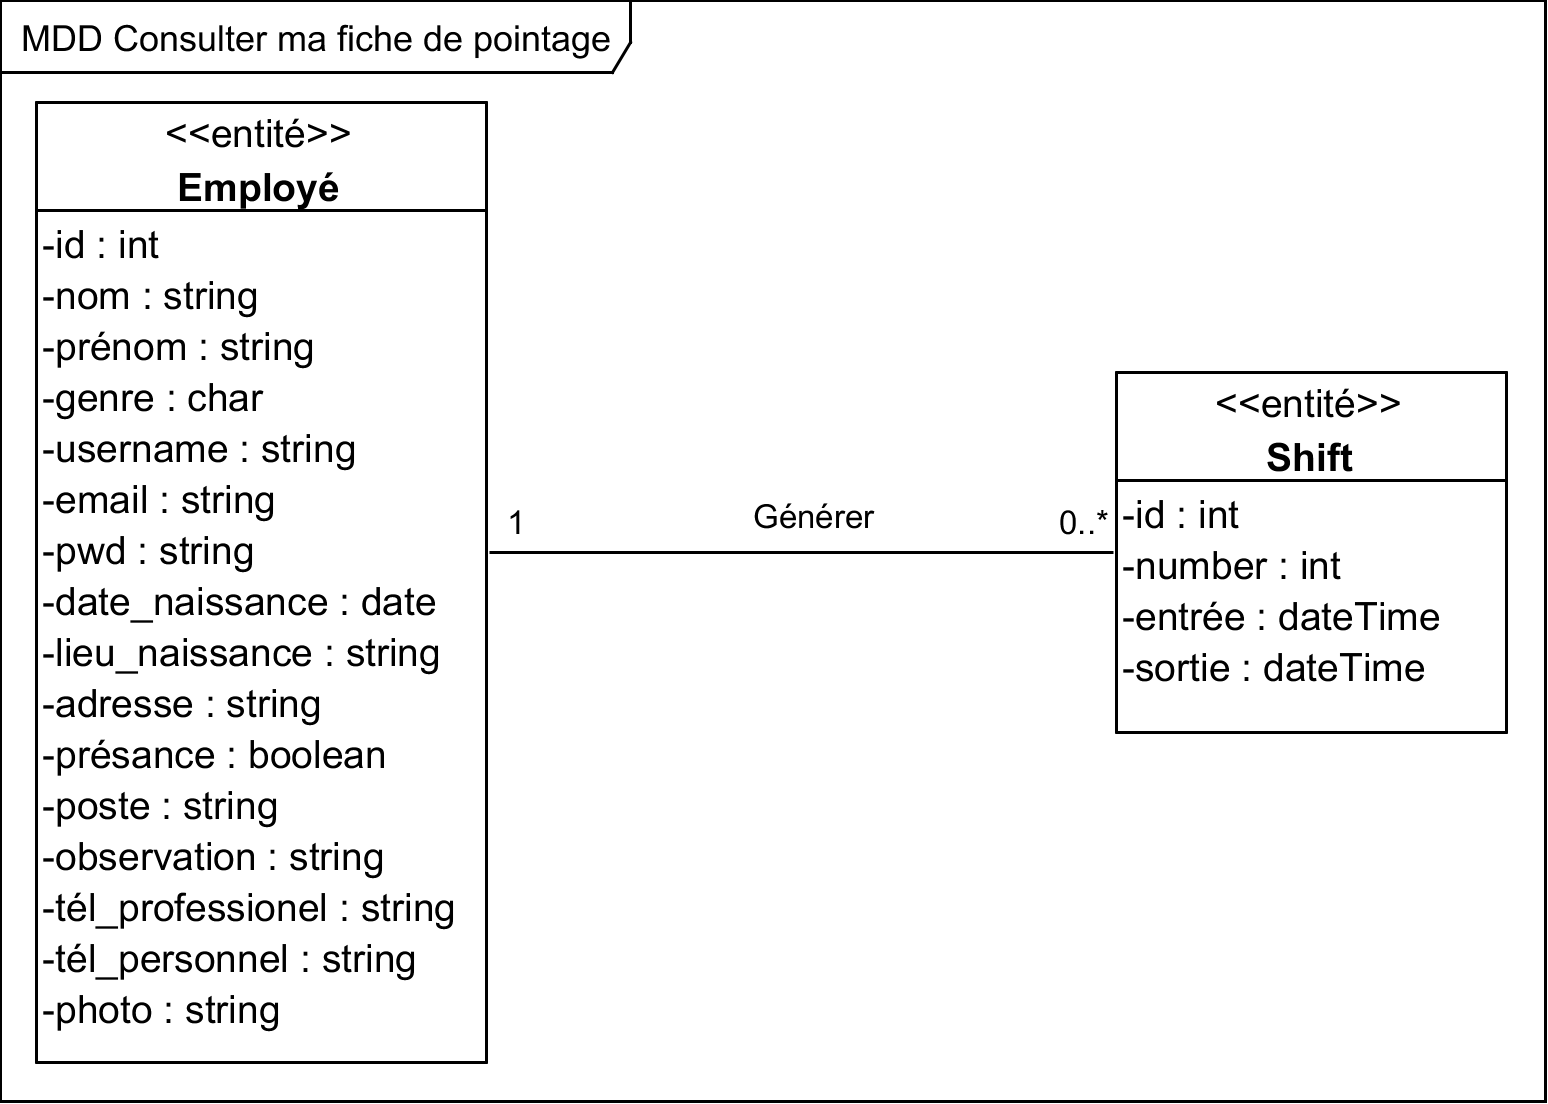
\includegraphics[scale=1.168]{images/MDD/MDD Consulter ma fiche de pointage.png}
    \caption{Modèle du domaine « Consulter ma fiche de pointage »}
    \label{fig13}
\end{figure}
            
\subsection*{Modèle du domaine du cas d'utilisation « Ajouter planning »}
Ce modèle du domaine exprime le fait qu’un planning est composé de sept jours. 
Dans lesquels nous retrouvons deux parties qui représente une journée de travail 
d’un employé.

\begin{figure}[h!]
    \centering
    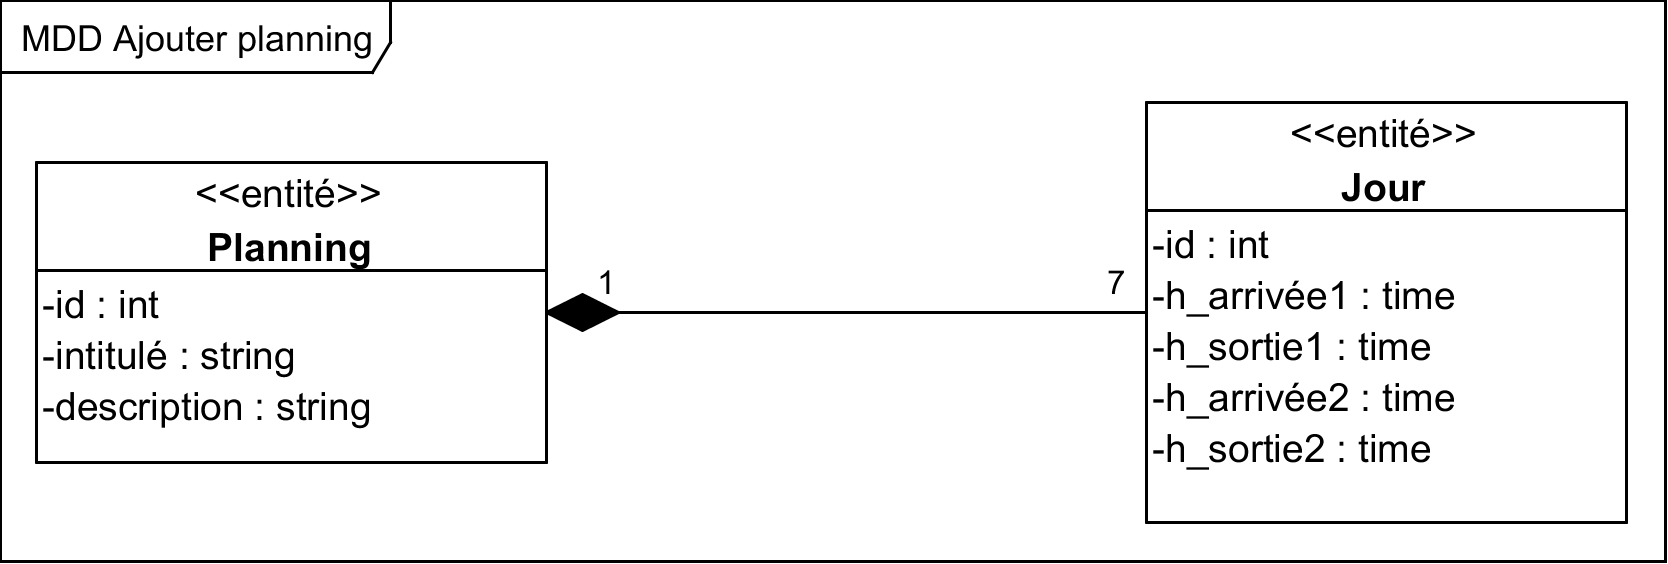
\includegraphics[scale=1.12]{images/MDD/MDD Ajouter planning.png}
    \caption{Modèle du domaine « Ajouter planning »}
    \label{fig14}
\end{figure}
        
\subsection*{Modèle du domaine du cas d'utilisation « Ajouter équipe »}
Sur ce modèle du domaine on remarque que les entités sont reliées par 
deux associations. Une représente le fait d’être membre d’une équipe, et 
l’autre le fait de gérer (ou manager) une équipe. Nous avons décidé de relier
cette association à l’employé et non au manager (qui hérite de l’employé), car
nous estimons qu’à ce stade il n’y a pas d'attributs liés exclusivement au
manager (il se pourrait que cela se fera dans les prochains diagrammes en raison
des méthodes).  

\begin{figure}[h!]
    \centering
    \includegraphics[scale=1.38]{images/MDD/MDD Ajouter équipe.png}
    \caption{Modèle du domaine « Ajouter équipe »}
    \label{fig15}
\end{figure}
            
\subsection*{Modèle du domaine du cas d'utilisation « Ajouter employé »}
Sur ce modèle du domaine figurent deux entités capitales de notre système 
qui sont l’employé et son empreinte. Il est important de noter qu’un employé 
ne peut avoir qu’une seule empreinte dans le système (index droit).

\clearpage

\begin{figure}[h!]
    \centering
    \includegraphics[scale=1.4]{images/MDD/MDD Ajouter employé.png}
    \caption{Modèle du domaine « Ajouter employé »}
    \label{fig16}
\end{figure}
            
\subsection*{Modèle du domaine du cas d'utilisation « Ajouter membre »}
En plus des deux entités, précédemment citées dans le modèle du domaine du cas 
d’utilisation « Ajouter équipe », on retrouve une classe d’association qui 
nous permet de garder une trace du changement d’équipe pour chaque employé.

\clearpage

\begin{figure}[h!]
	\centering
	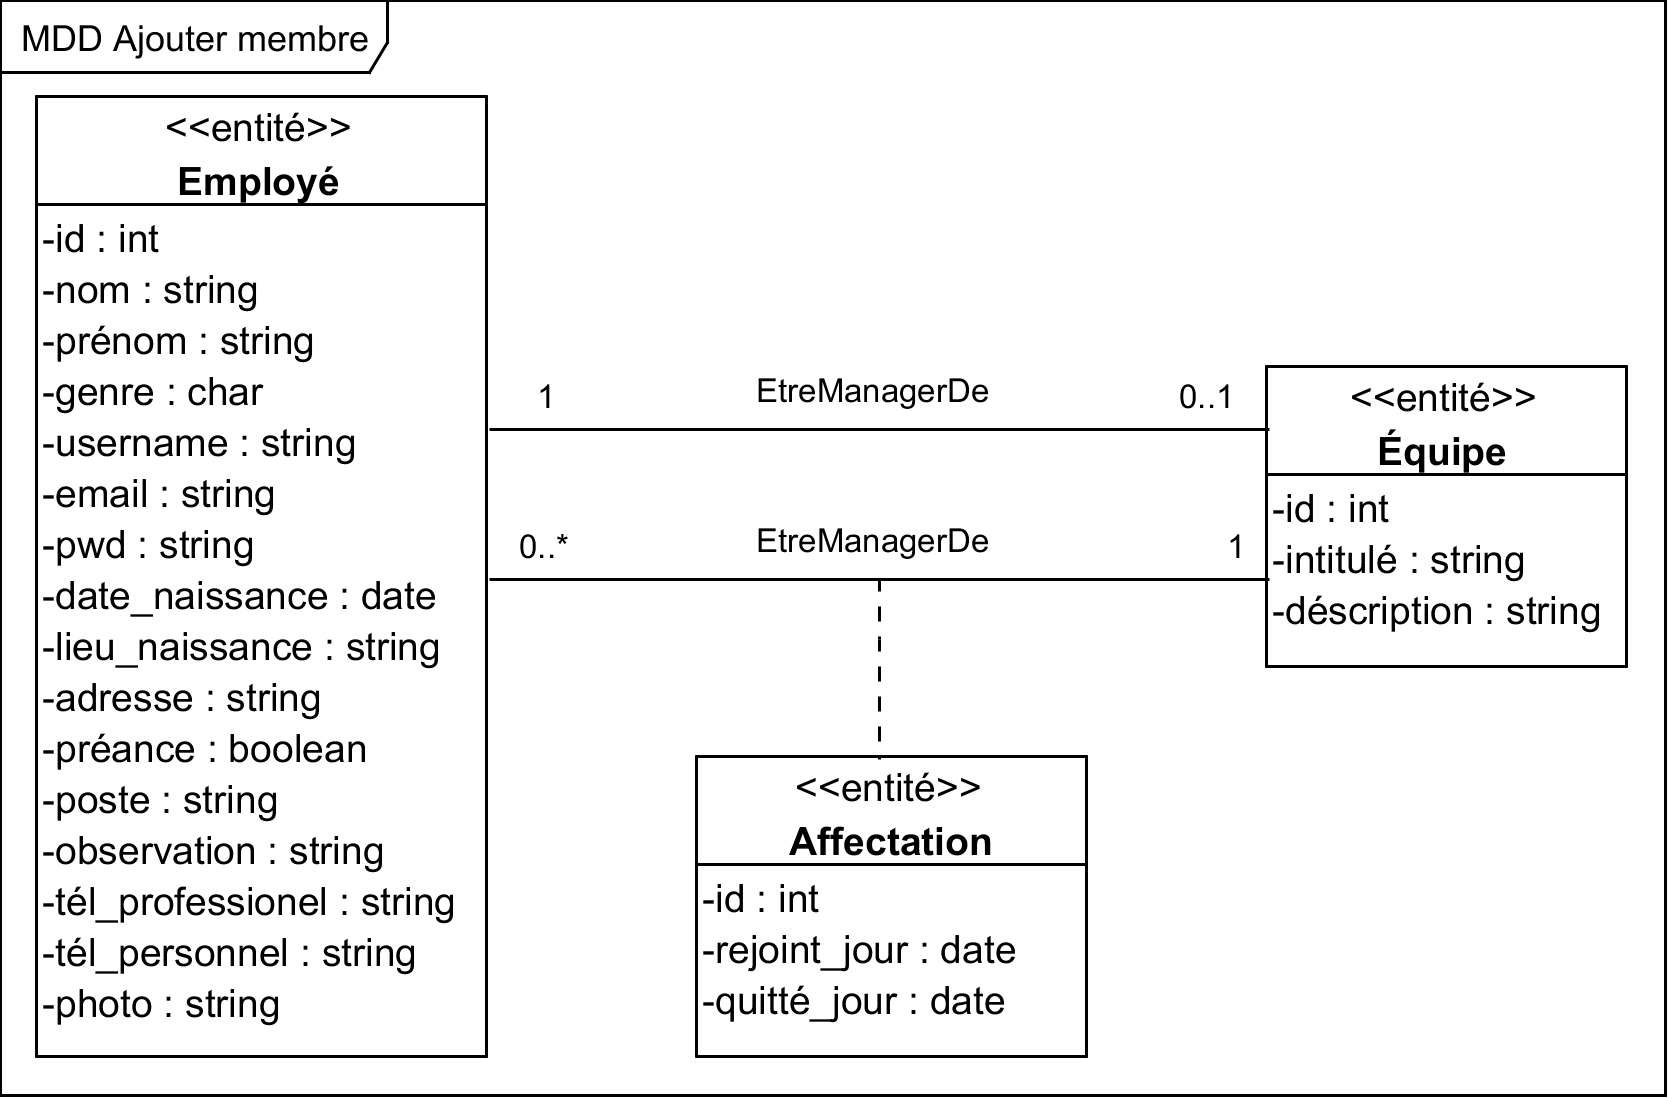
\includegraphics[scale=1.22]{images/MDD/MDD Ajouter membre.png}
	\caption{Diagramme de séquence système « Ajouter membre »}
	\label{fig17}
\end{figure}


\subsection*{Modèle du domaine du cas d'utilisation « Consulter profil d'un employé »}
Sur ce modèle du domaine, le but est d’offrir aux employés un planning 
flexible. Pour ce faire, nous avons une composition entre 2 entités: un
\emph{planning} qui est la classe mère avec comme attributs un intitulé du
planning ainsi qu’une description, et une classe \emph{jour} qui modélise les
jours de la semaine avec comme attributs les horaires de travails.

\clearpage

\begin{figure}[h!]
    \centering
    \includegraphics[scale=1.32]{images/MDD/MDD Consulter profil d'un employé.png}
    \caption{Modèle du domaine « Consulter profil d'un employé »}
    \label{fig18}
\end{figure}
            
\subsection*{Modèle du domaine du cas d'utilisation « Consulter tableau de bord manager »}
Sur ce modèle du domaine, on peut observer que plusieurs entités participent à
la réalisation du cas d’utilisation. Ceci est dû à sa nature sommaire. Un
tableau de bord se doit d’être récapitulatif et offrir un maximum d’informations
pertinentes en un minimum d’espace. Pour avoir la liste des collaborateurs, nous
avons besoins des deux entités: \emph{employé} et \emph{équipe}. Afin de savoir
si un collaborateur est en retard ou absent, on doit accéder à son planning. 

\begin{figure}[h!]
    \centering
    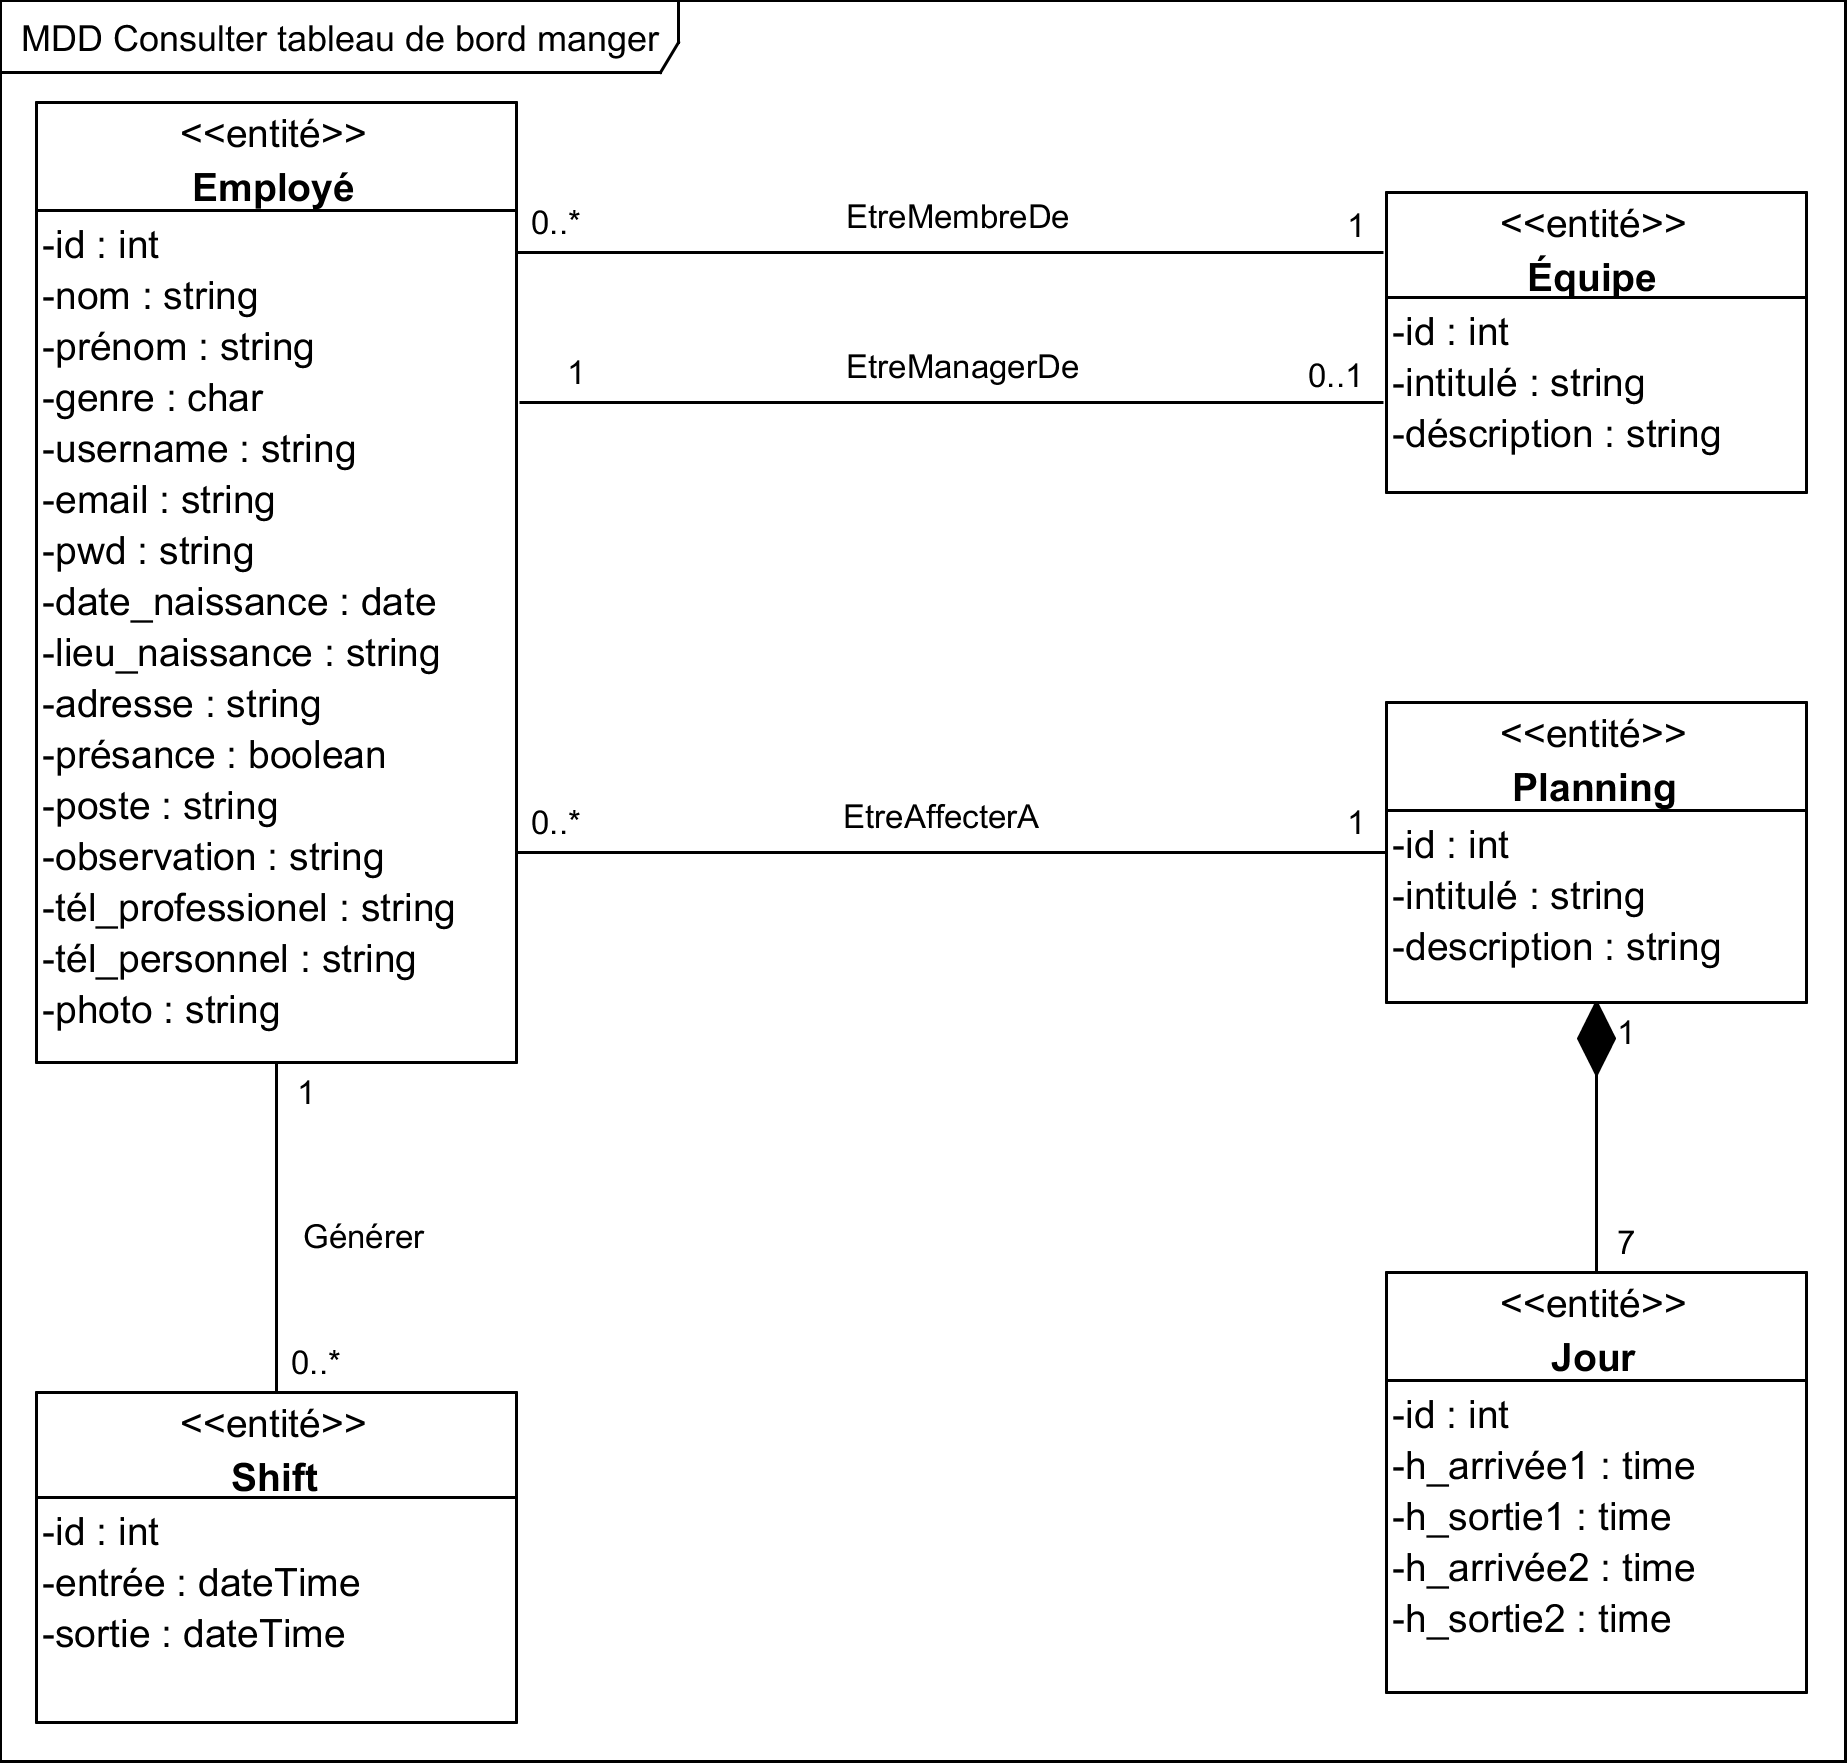
\includegraphics[scale=1.06]{images/MDD/MDD Consulter tableu de bord manger.png}
    \caption{Modèle du domaine « Consulter tableau de bord manager »}
    \label{fig19}
\end{figure}
            
\section{Diagrammes de classes participantes}
L’importance du diagramme de classes participantes réside dans le fait qu’il
effectue la jonction entre les cas d’utilisation, les classes d’analyse et
l’interface avec l’utilisateur, de plus, il permet l’enrichissement des
diagrammes de séquence système.\cite{8}

\subsection{Définitions et formalisme}
Les classes composant un diagramme de classes participantes se répartissent en
trois catégories:\cite{6}

\subsubsection{Les classes de dialogue}
Ces classes permettent les interactions entre l’IHM et les utilisateurs. 
Il s’agit typiquement des écrans proposés à l’utilisateur: les formulaires de 
saisie, les résultats de recherche, etc. En général, les dialogues vivent 
seulement le temps du déroulement du cas d’utilisation concerné, afin de 
modéliser une classe de dialogue nous allons utiliser le modèle de la 
figure\ref{fig20}.

\begin{figure}[h!]
    \centering
    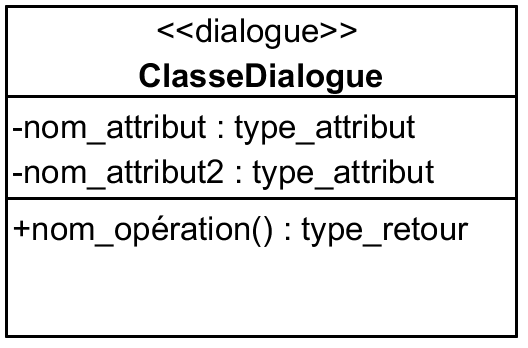
\includegraphics[scale=1.5]{images/dialogue.png}
    \caption{Représentation d'une classe dialogue}
    \label{fig20}
\end{figure}
        
\subsubsection{Les classes de contrôle}
Les classes qui modélisent la cinématique de l’application sont appelées 
contrôles. Elles font la jonction entre les dialogues et les classes métier en 
permettant aux différentes vues de l’application de manipuler des informations 
détenues par des objets métier. Elles contiennent les règles applicatives et les 
isolent à la fois des dialogues et des entités, elles seront représentées comme 
sur la figure\ref{fig21}.

\begin{figure}[h!]
    \centering
    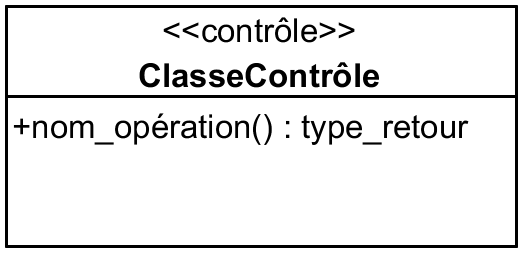
\includegraphics[scale=1.5]{images/Controle.png}
    \caption{Représentation d'une classe contrôle}
    \label{fig21}
\end{figure}
        
\subsubsection{Les classes entités}
Les classes métier, qui proviennent directement du modèle du domaine sont 
qualifiées d’entités. Ces classes sont généralement persistantes, 
c’est à dire qu’elles survivent à l’exécution d’un cas d’utilisation 
particulier et qu’elles permettent à des données et à des relations d’être 
stockées dans des fichiers ou des bases de données. Elles seront 
représentées comme sur la figure\ref{fig22}.

\clearpage

\begin{figure}[h!]
    \centering
    \includegraphics[scale=1.5]{images/Entité.png}
    \caption{Représentation d'une classe entité}
    \label{fig22}
\end{figure}
        
Afin d’établir un DCP, nous ajouterons des associations entre les classes tout 
en respectant les règles ci-après: \cite{5}

\begin{itemize}
    \item[\textbullet] Les dialogues ne peuvent être reliés qu'aux contrôles ou à 
        d'autres dialogues, mais pas directement aux entités.
    \item [\textbullet] Les entités ne peuvent être reliées qu'aux contrôles ou à 
        d'autres entités.
    \item [\textbullet] Les contrôles ont accès à tous les types de classes, y 
        compris d'autres contrôles.
    \item [\textbullet] Enfin, un acteur ne peut être lié qu'à un dialogue.
\end{itemize}

Un exemple de diagramme de classe participante est représenté dans la figure 
ci-dessous:  

\begin{figure}[h!]
    \centering
    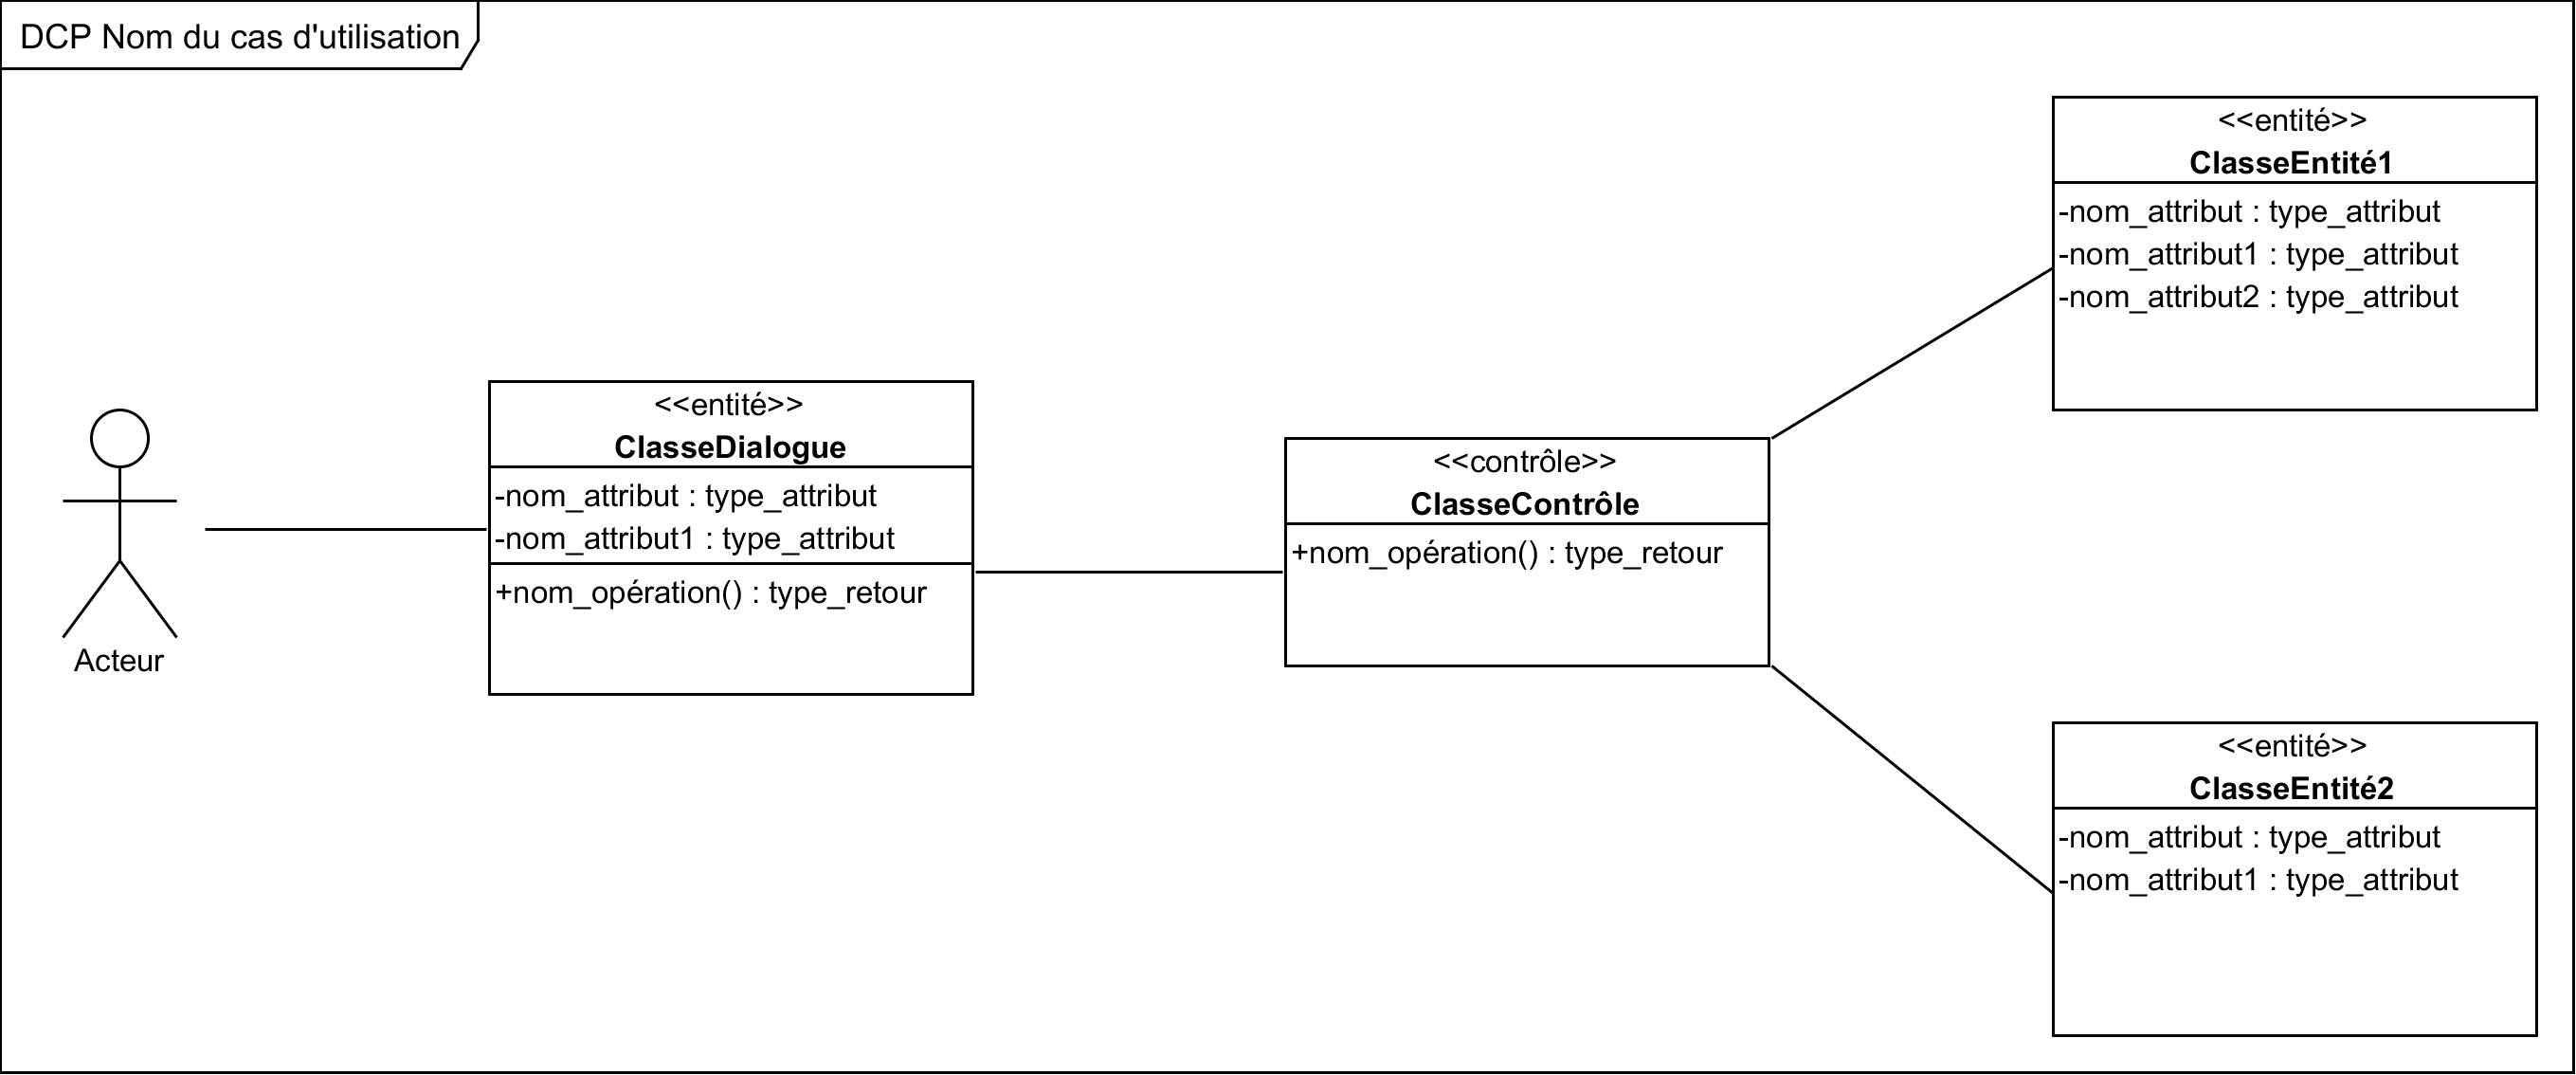
\includegraphics[scale=0.74]{images/DCP_exemple.png}
    \caption{Modèle d'un diagramme de classe de conception}
    \label{fig23}
\end{figure}

\clearpage

\subsection*{Diagrammes de classes participantes du cas d'utilisation « Se pointer »}
La pointeuse biométrique permet à l’employé d’enregistrer ses horaires de 
travails le plus facilement possible. Pour ce qui est de la logique concernant 
les actions effectuées par l’employé, elle est déléguée à trois contrôleurs: 
CtrShift et CtrEmployé et CtrEmpreinte.
            
\begin{figure}[h!]
    \centering
    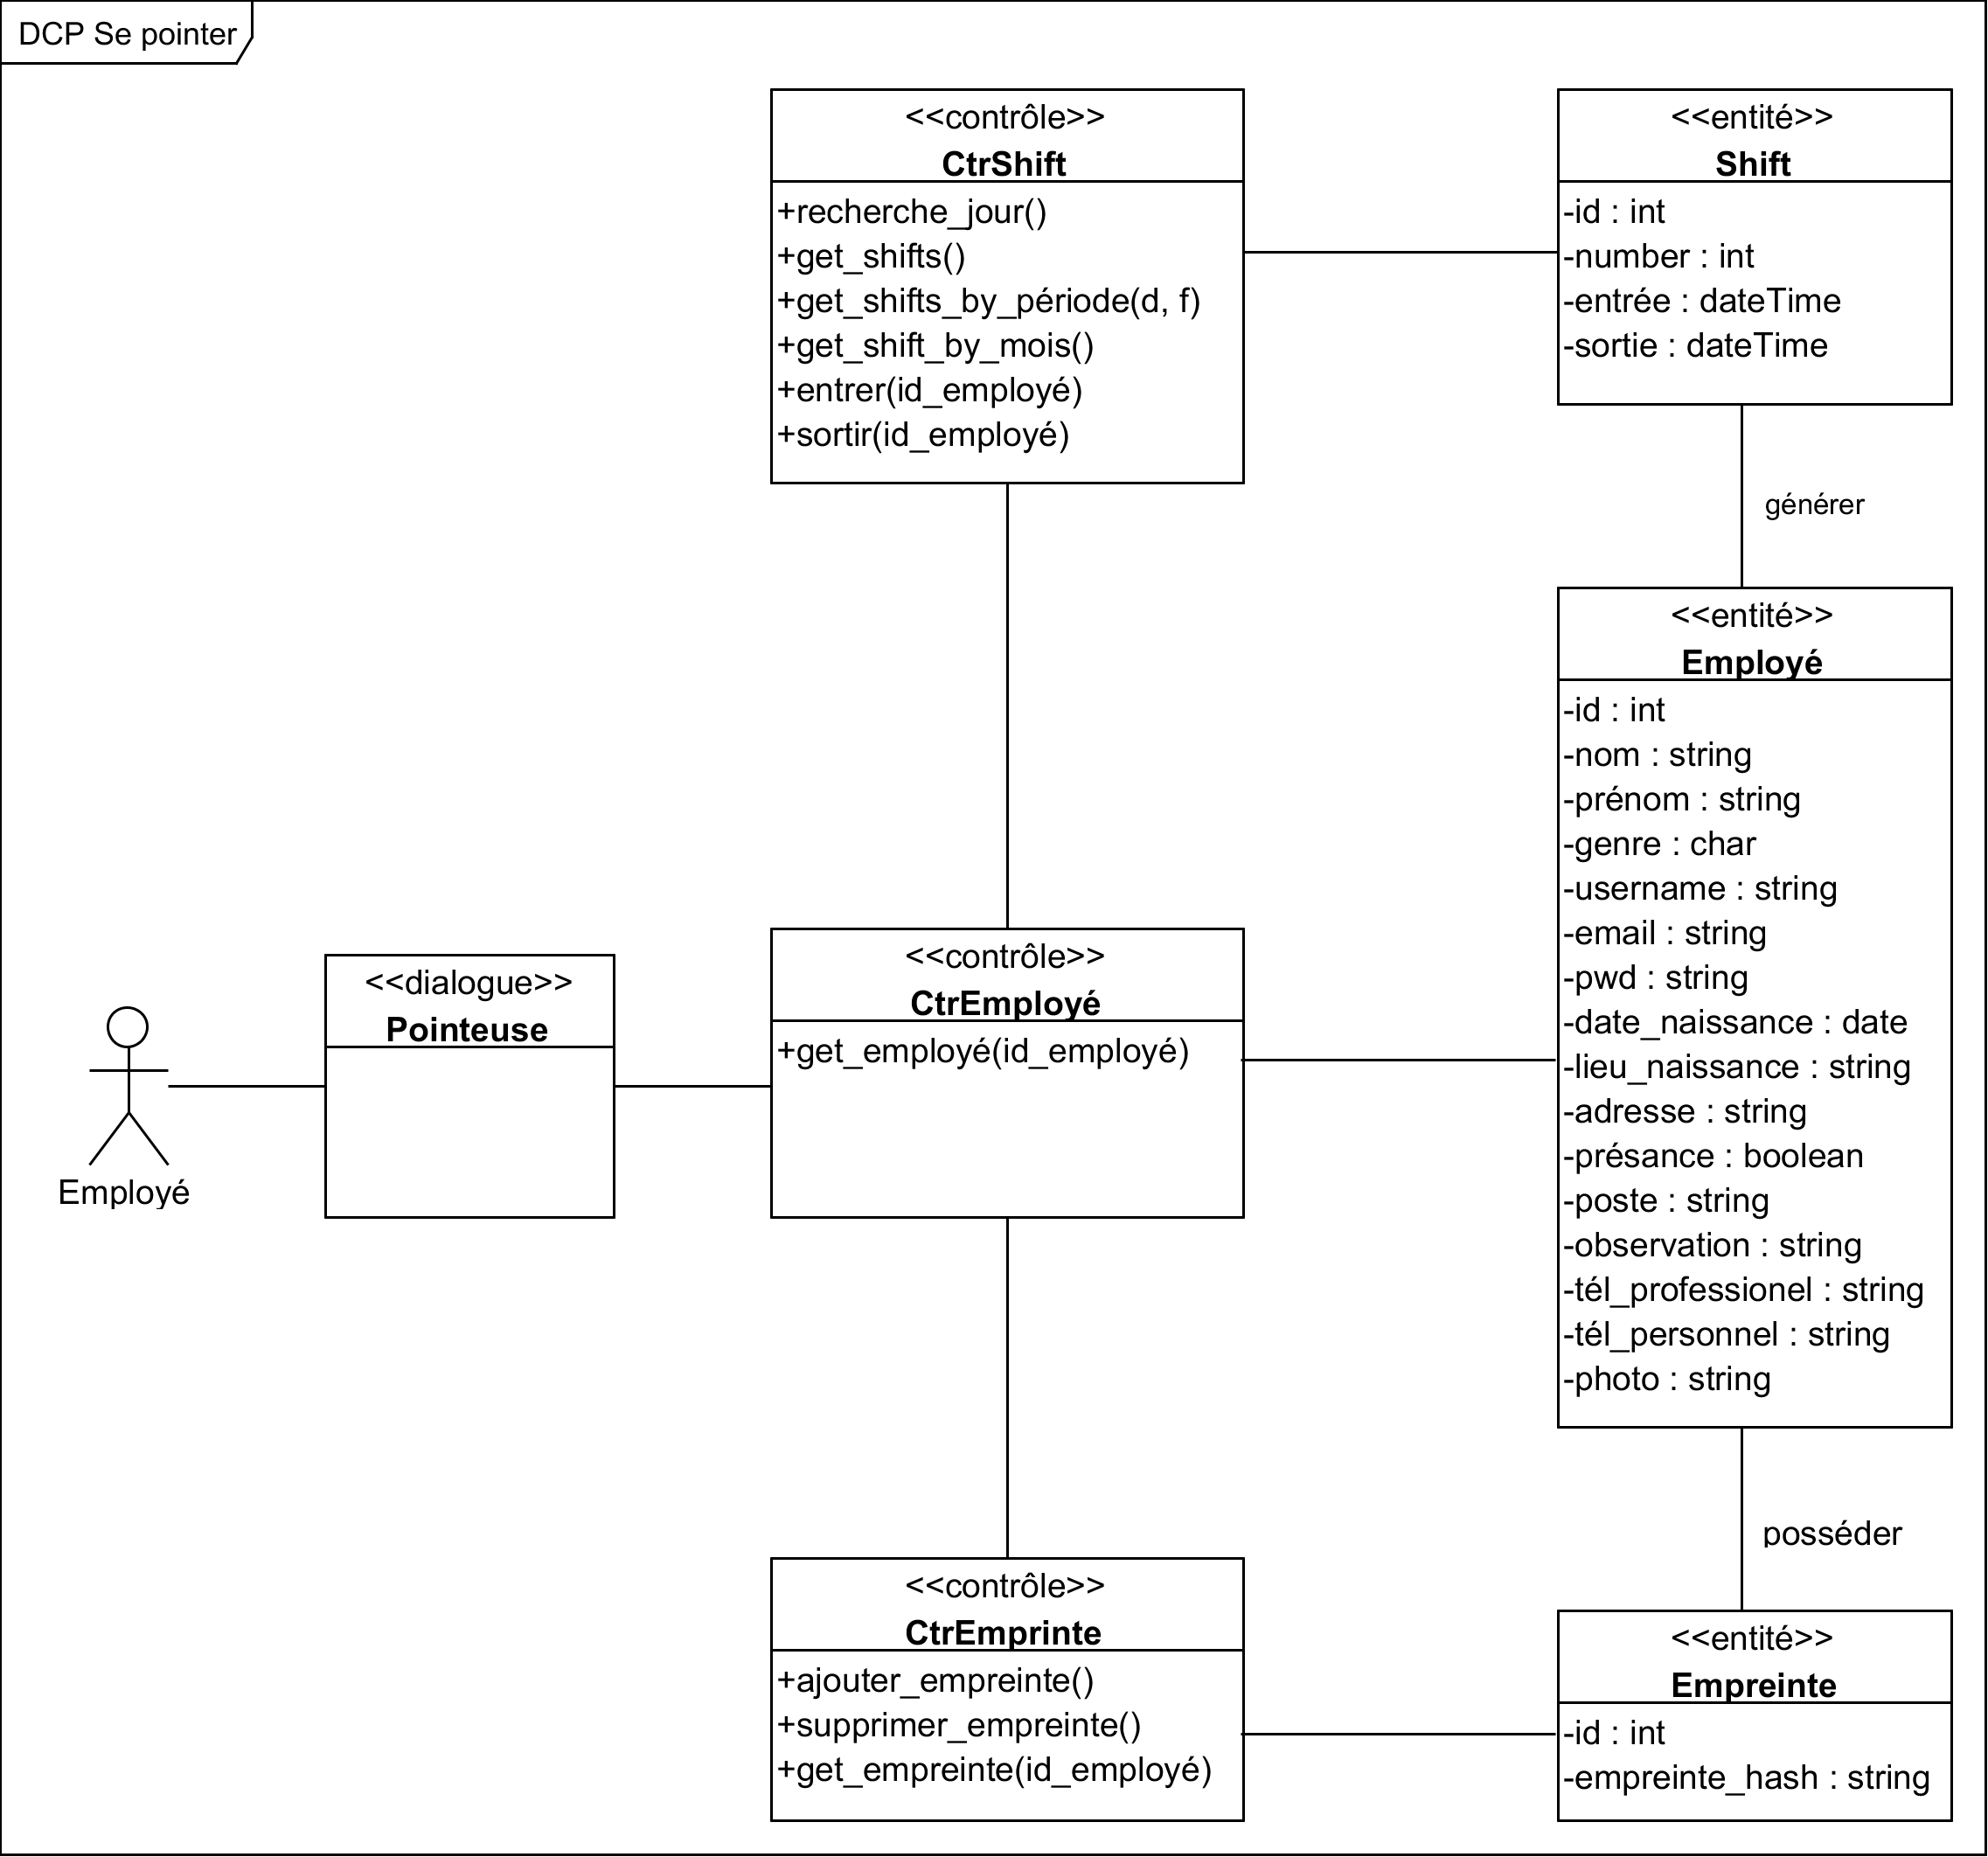
\includegraphics[scale=0.84]{images/DCP/DCP Se pointer.png}
    \caption{Diagrammes de classes participantes « Consulter ma fiche de pointage »}
    \label{fig24}
\end{figure}
            
\subsection*{Diagrammes de classes participantes du cas d'utilisation « Consulter mon profil »}
Un employé peut consulter son profil sur l’interface « InterfaceMonProfil » qui 
regroupe ses informations, il peut aussi accéder à l’interface de modification 
de son profil, ainsi qu’afficher son planning. Les actions effectuées sont 
gérées par le contrôleur CtrEmployé.  

\begin{figure}[h!]
    \centering
    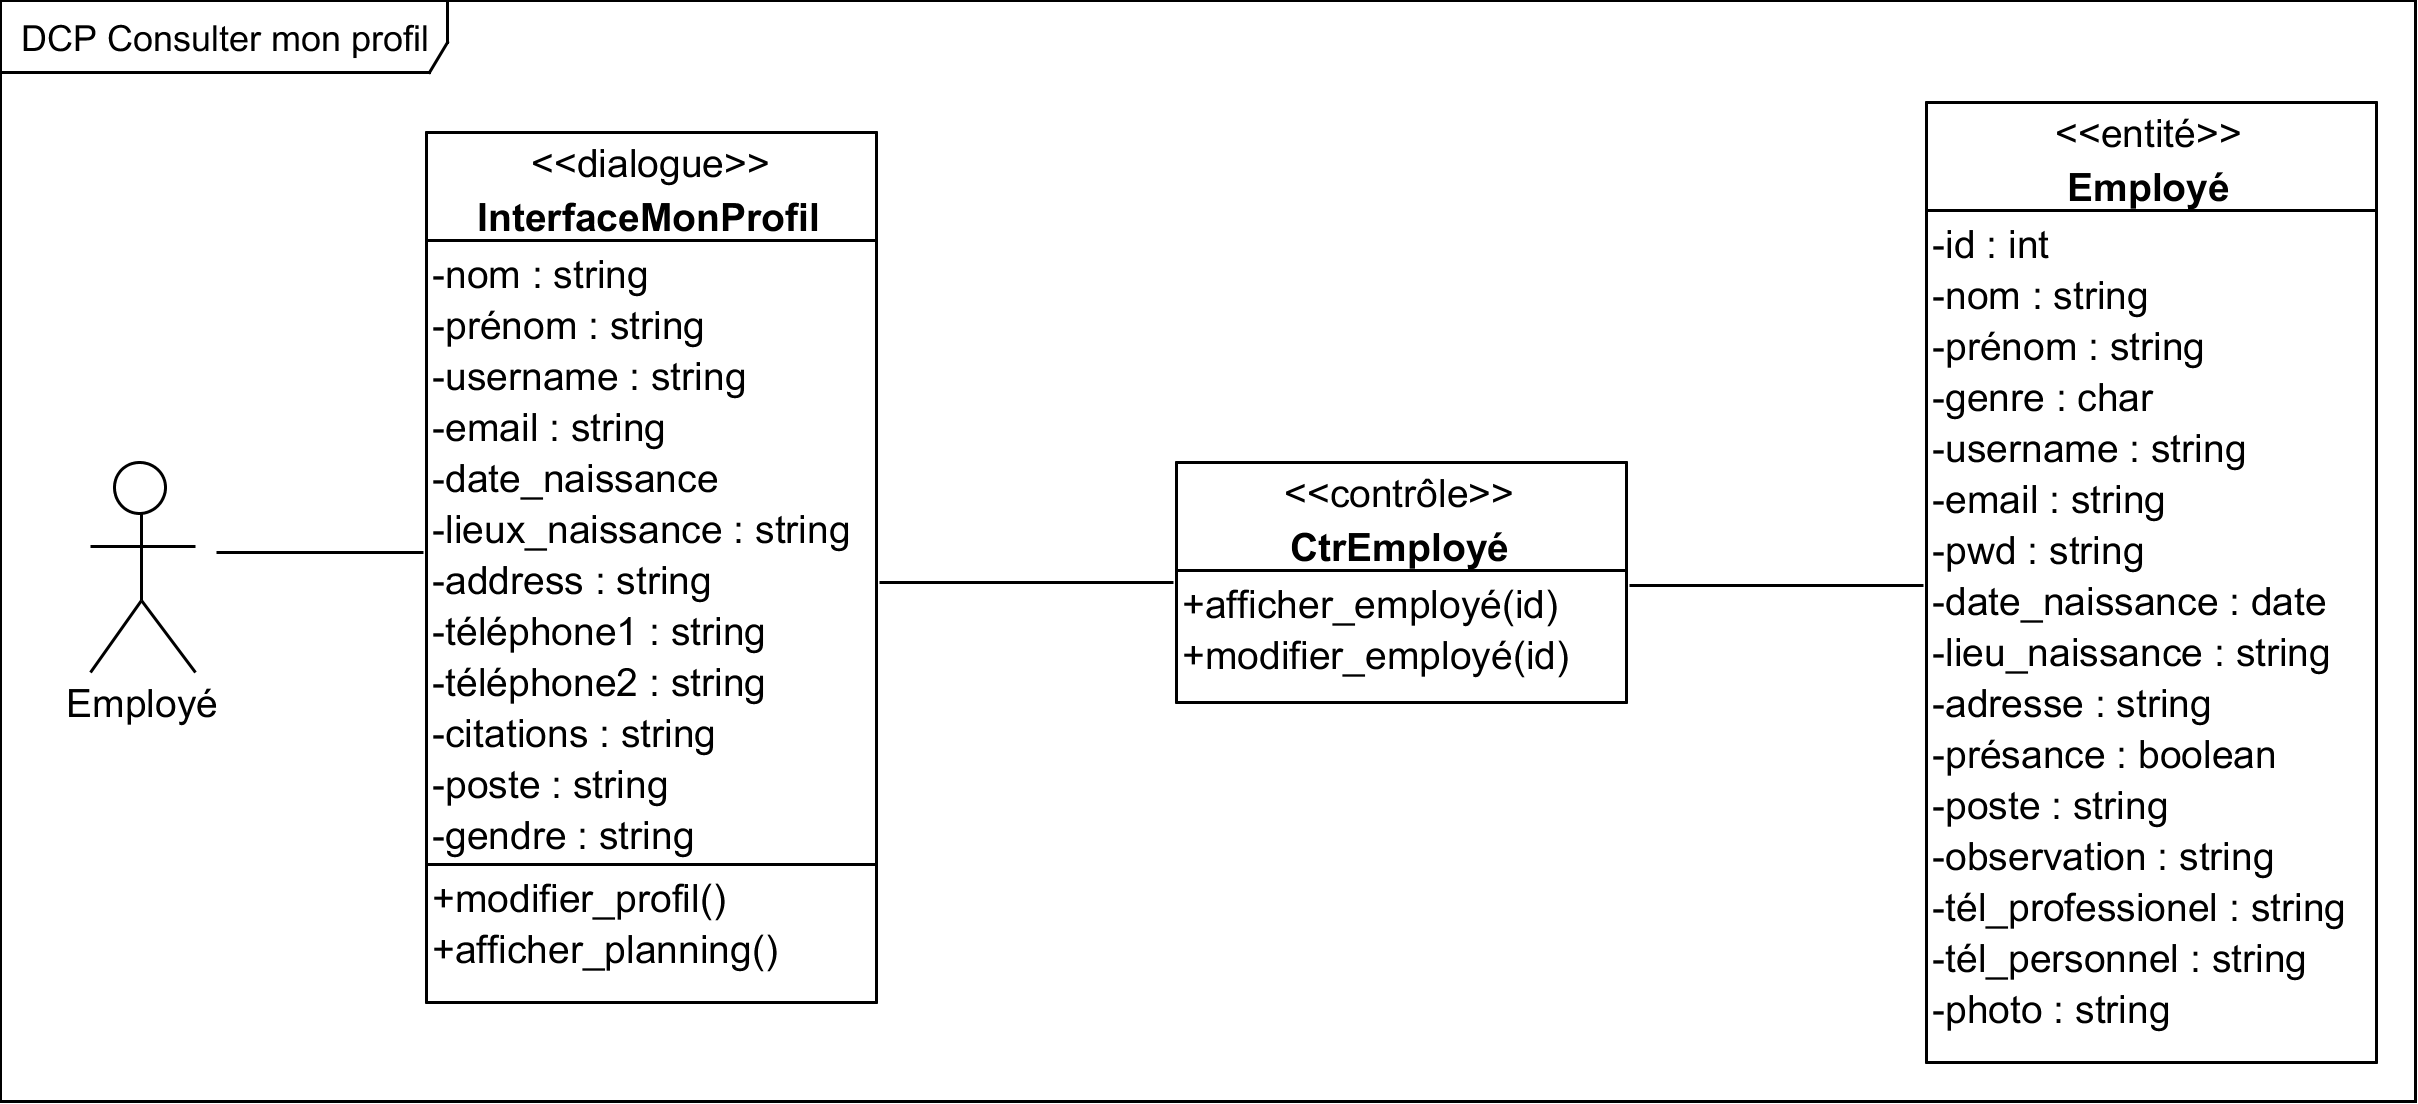
\includegraphics[scale=0.7]{images/DCP/DCP consulter_mon_profil.png}
    \caption{Diagrammes de classes participantes « Consulter mon profil »}
    \label{fig25}
\end{figure}
        
\subsection*{Diagrammes de classes participantes du cas d'utilisation « Consulter ma fiche de pointage »}
Un employé peut consulter sa fiche de pointage sur l’interface «
InterfaceConsulterMaFichePointage ». Par défaut, l’affichage de la liste des
pointages est par semaine, s’il le souhaite il peut l’afficher par mois ou faire
une recherche précise par période. La logique concernant les actions effectuées
par l’employé est déléguée à deux contrôleurs: CtrShift et CtrEmployé.
            
\begin{figure}[h!]
    \centering
    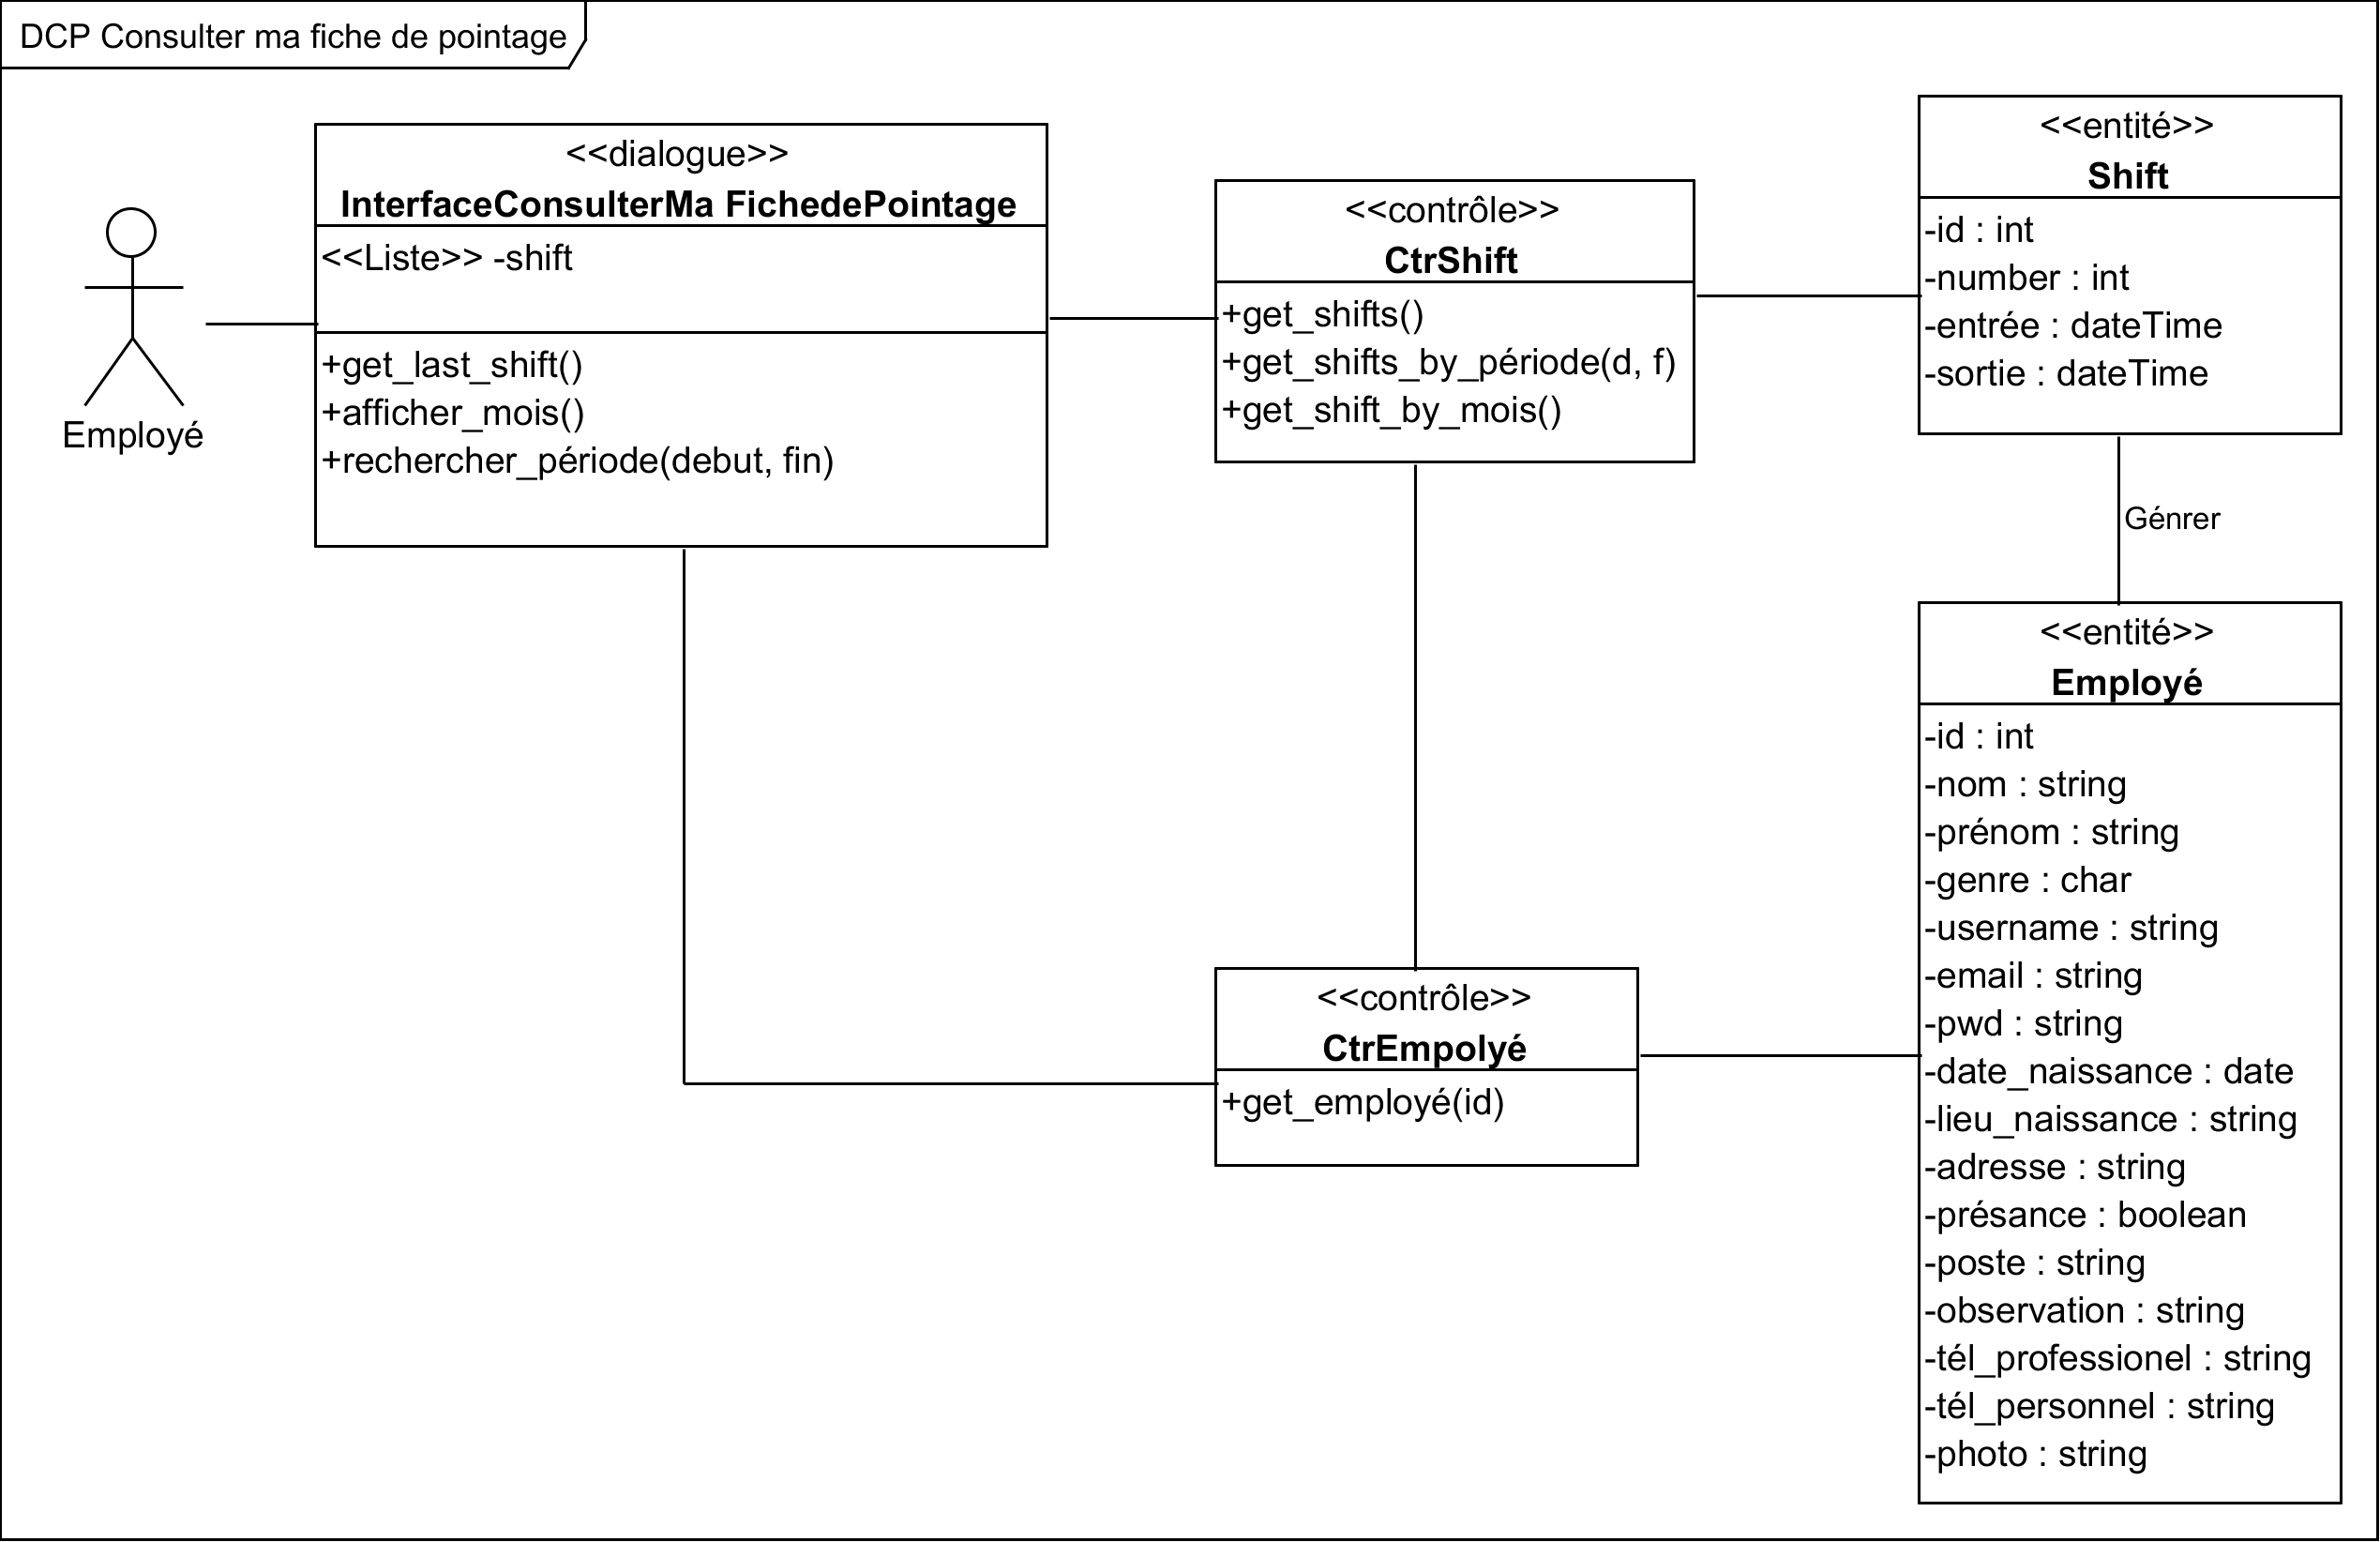
\includegraphics[scale=0.72]{images/DCP/DCP Consulter ma fiche de pointage.png}
    \caption{Diagrammes de classes participantes « Consulter ma fiche de pointage »}
    \label{fig26}
\end{figure}
            
\subsection*{Diagrammes de classes participantes du cas d'utilisation « Consulter tableau de bord manager »}
Une fois authentifié, le manager est redirigé vers 
« InterfaceTableauBordManager » où il aura accès à son planning du jour, une 
liste de ces collaborateurs, ainsi qu’un résumé sur l’ensemble de ces équipes. 
Les 2 contrôles CtrEmployés et CtrEquipe traitent les actions du manager. 

\begin{figure}[h!]
    \centering
    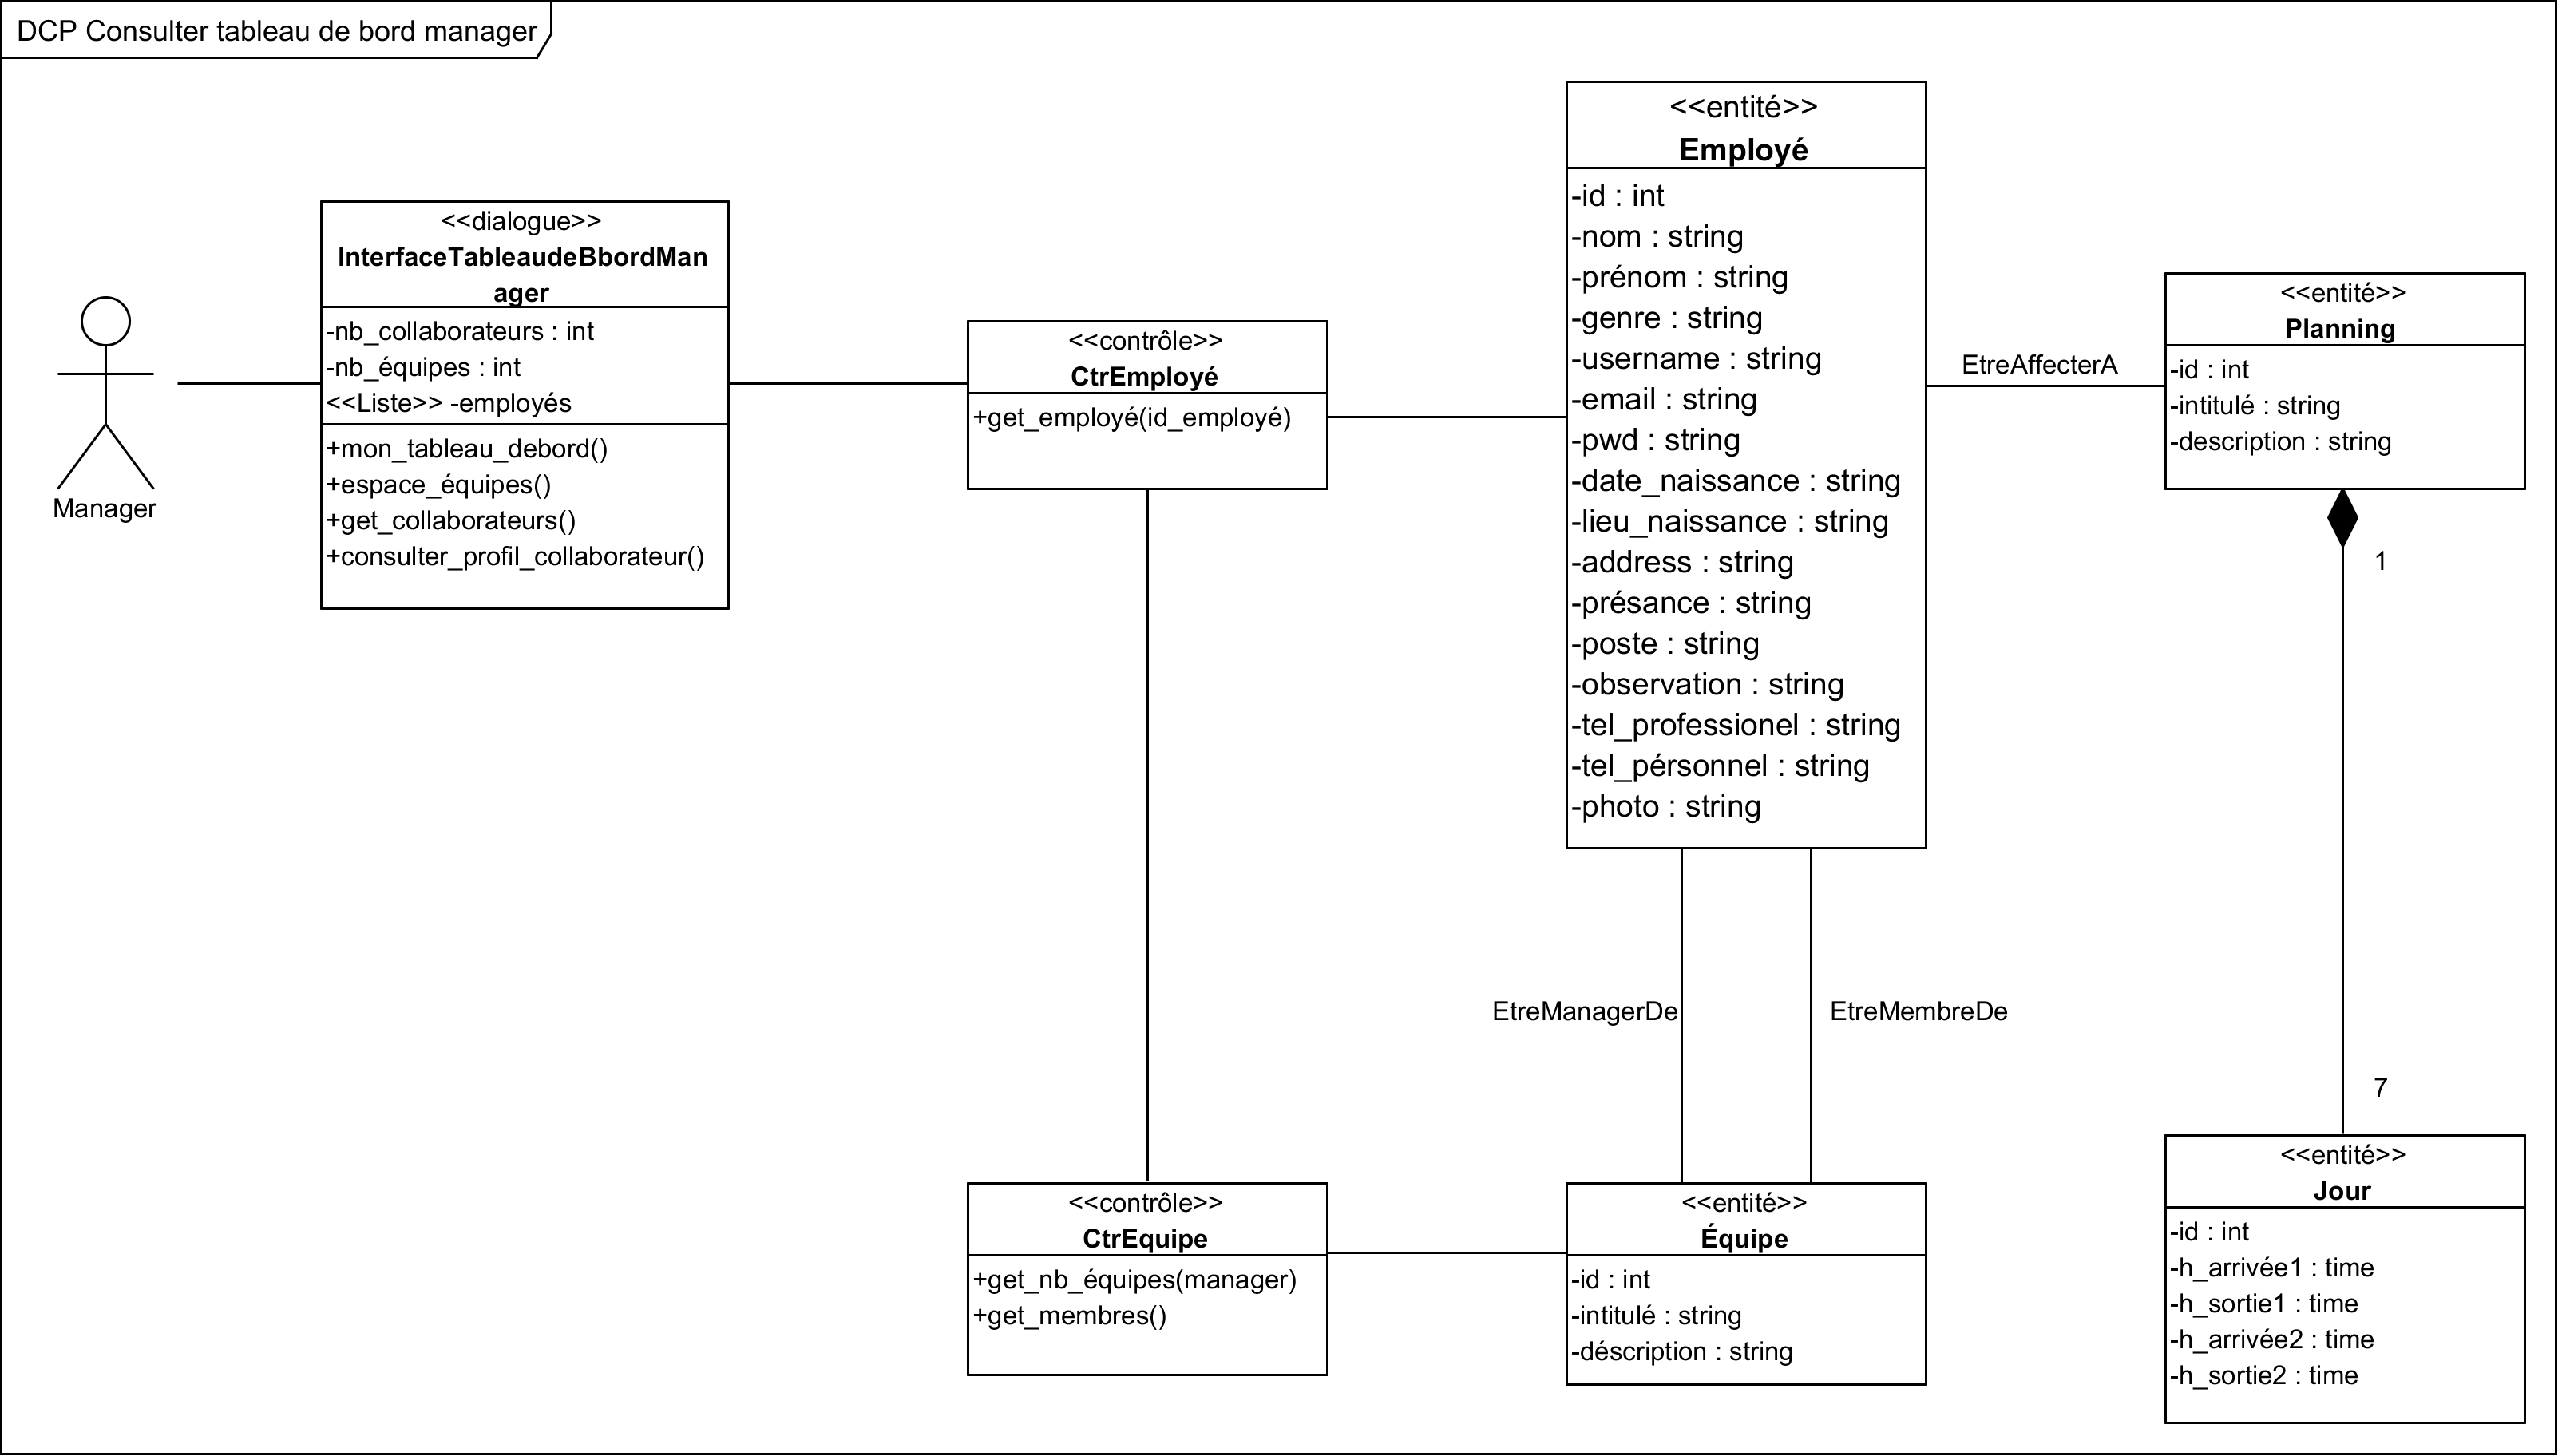
\includegraphics[scale=0.68,angle=90]{images/DCP/DCP Consulter tableau de bord manager.png}
    \caption{Diagrammes de classes participantes « Consulter tableau de bord manager »}
    \label{fig27}
    \end{figure}

\clearpage
       
\subsection*{Diagrammes de classes participantes du cas d'utilisation « Ajouter planning »}
L’interface « InterfaceAjouterPlanning » affiche un formulaire qui permet à
l’acteur de créer un nouveau planning. Il doit saisir le nom, la description,
ainsi que les différents horaires de travail. Une fois validé par l’acteur,
CtrPlanning vérifie les informations saisies pour enfin pouvoir ajouter le
planning à son entité correspondante.
           
\begin{figure}[h!]
    \centering
    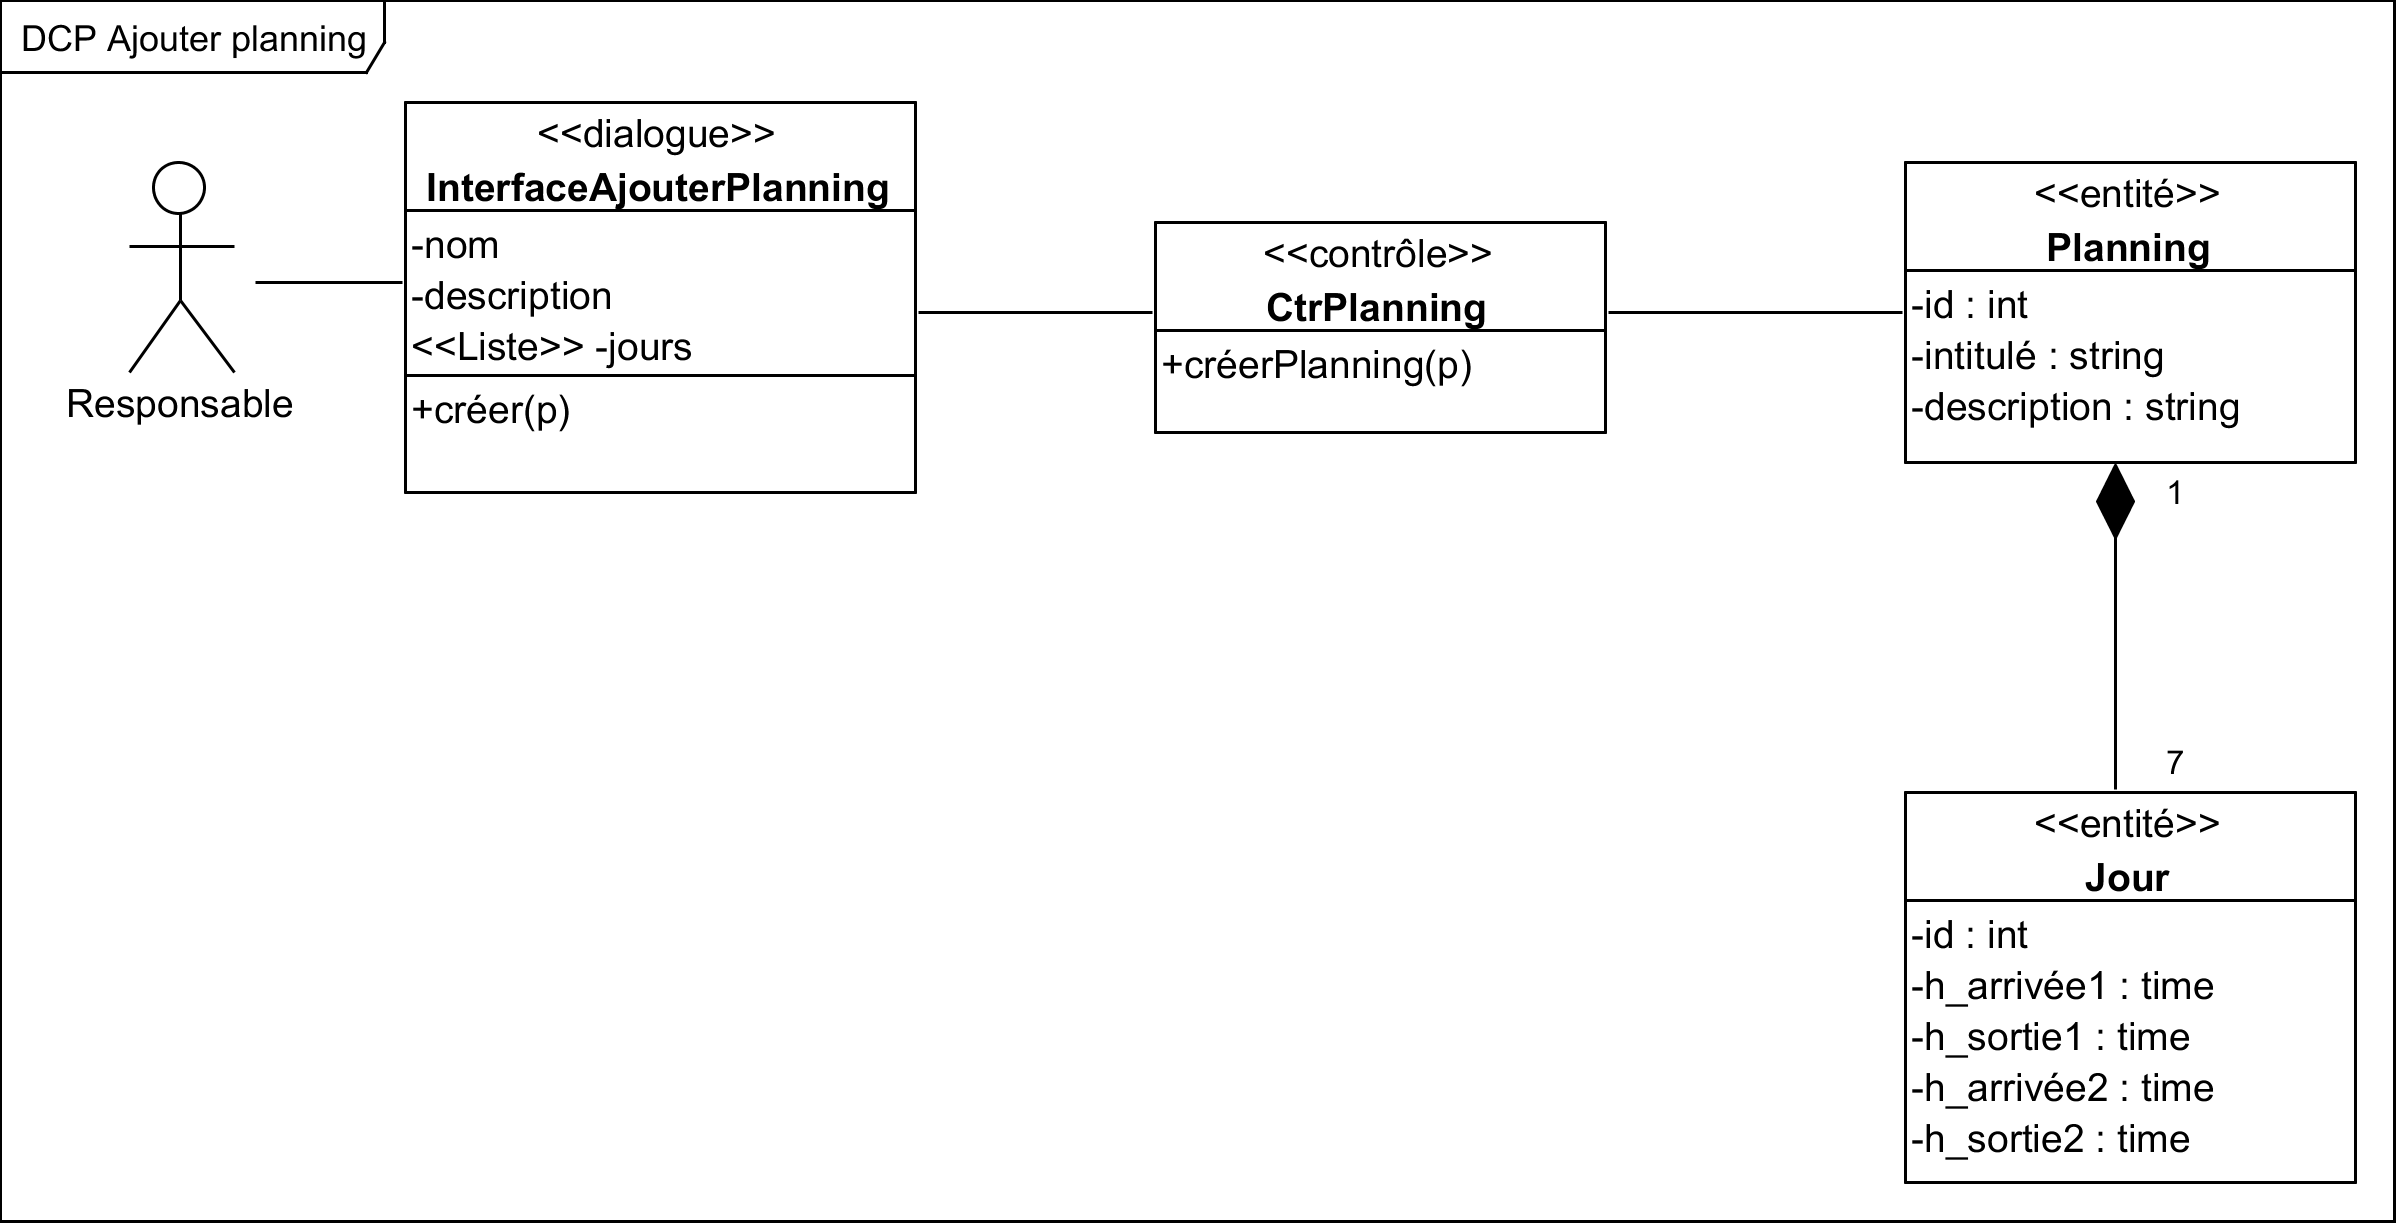
\includegraphics[scale=0.88]{images/DCP/DCP Ajouter planning.png}
    \caption{Diagrammes de classes participantes « Ajouter planning »}
    \label{fig28}
\end{figure}
        
\subsection*{Diagrammes de classes participantes du cas d'utilisation « Ajouter équipe »}
L’interface « InterfaceAjouterEquipe » affiche un formulaire qui permet à
l’acteur de créer une nouvelle équipe. Il doit saisir le nom, la description
ainsi que chercher et sélectionner un manager qui sera le responsable de cette
dernière.
        
La logique concernant les actions effectuées par l’acteur est déléguée à 
deux contrôleurs, CtrEmployé qui va gérer la recherche du manager et CtrEquipe
qui vérifiera les informations saisies pour pouvoir ajouter l’équipe à son 
entité correspondante.
       
\clearpage
            
\begin{figure}[h!]
    \centering
    \includegraphics[scale=0.85]{images/DCP/DCP Ajouter équipe.png}
    \caption{Diagrammes de classes participantes « Ajouter équipe »}
    \label{fig29}
\end{figure}
            
\subsection*{Diagrammes de classes participantes du cas d'utilisation « Ajouter membre »}
L’interface « InterfaceAjouterMembre » affiche à l’acteur une liste des membres 
de l’équipe, ainsi qu’un champ qui lui permettra de faire une recherche d’un 
employé afin de l’ajouter à l’équipe.
        
Pour ce qui est des classes de contrôles, la première classe CtrEquipe aura la 
responsabilité de gérer la recherche, et l’ajout des membres de l’équipe. Quant
à la deuxième classe CtrAffectation, elle permettra de créer une affectation pour 
chaque employé ajouter.
       
\clearpage
            
\begin{figure}[h!]
	\centering
    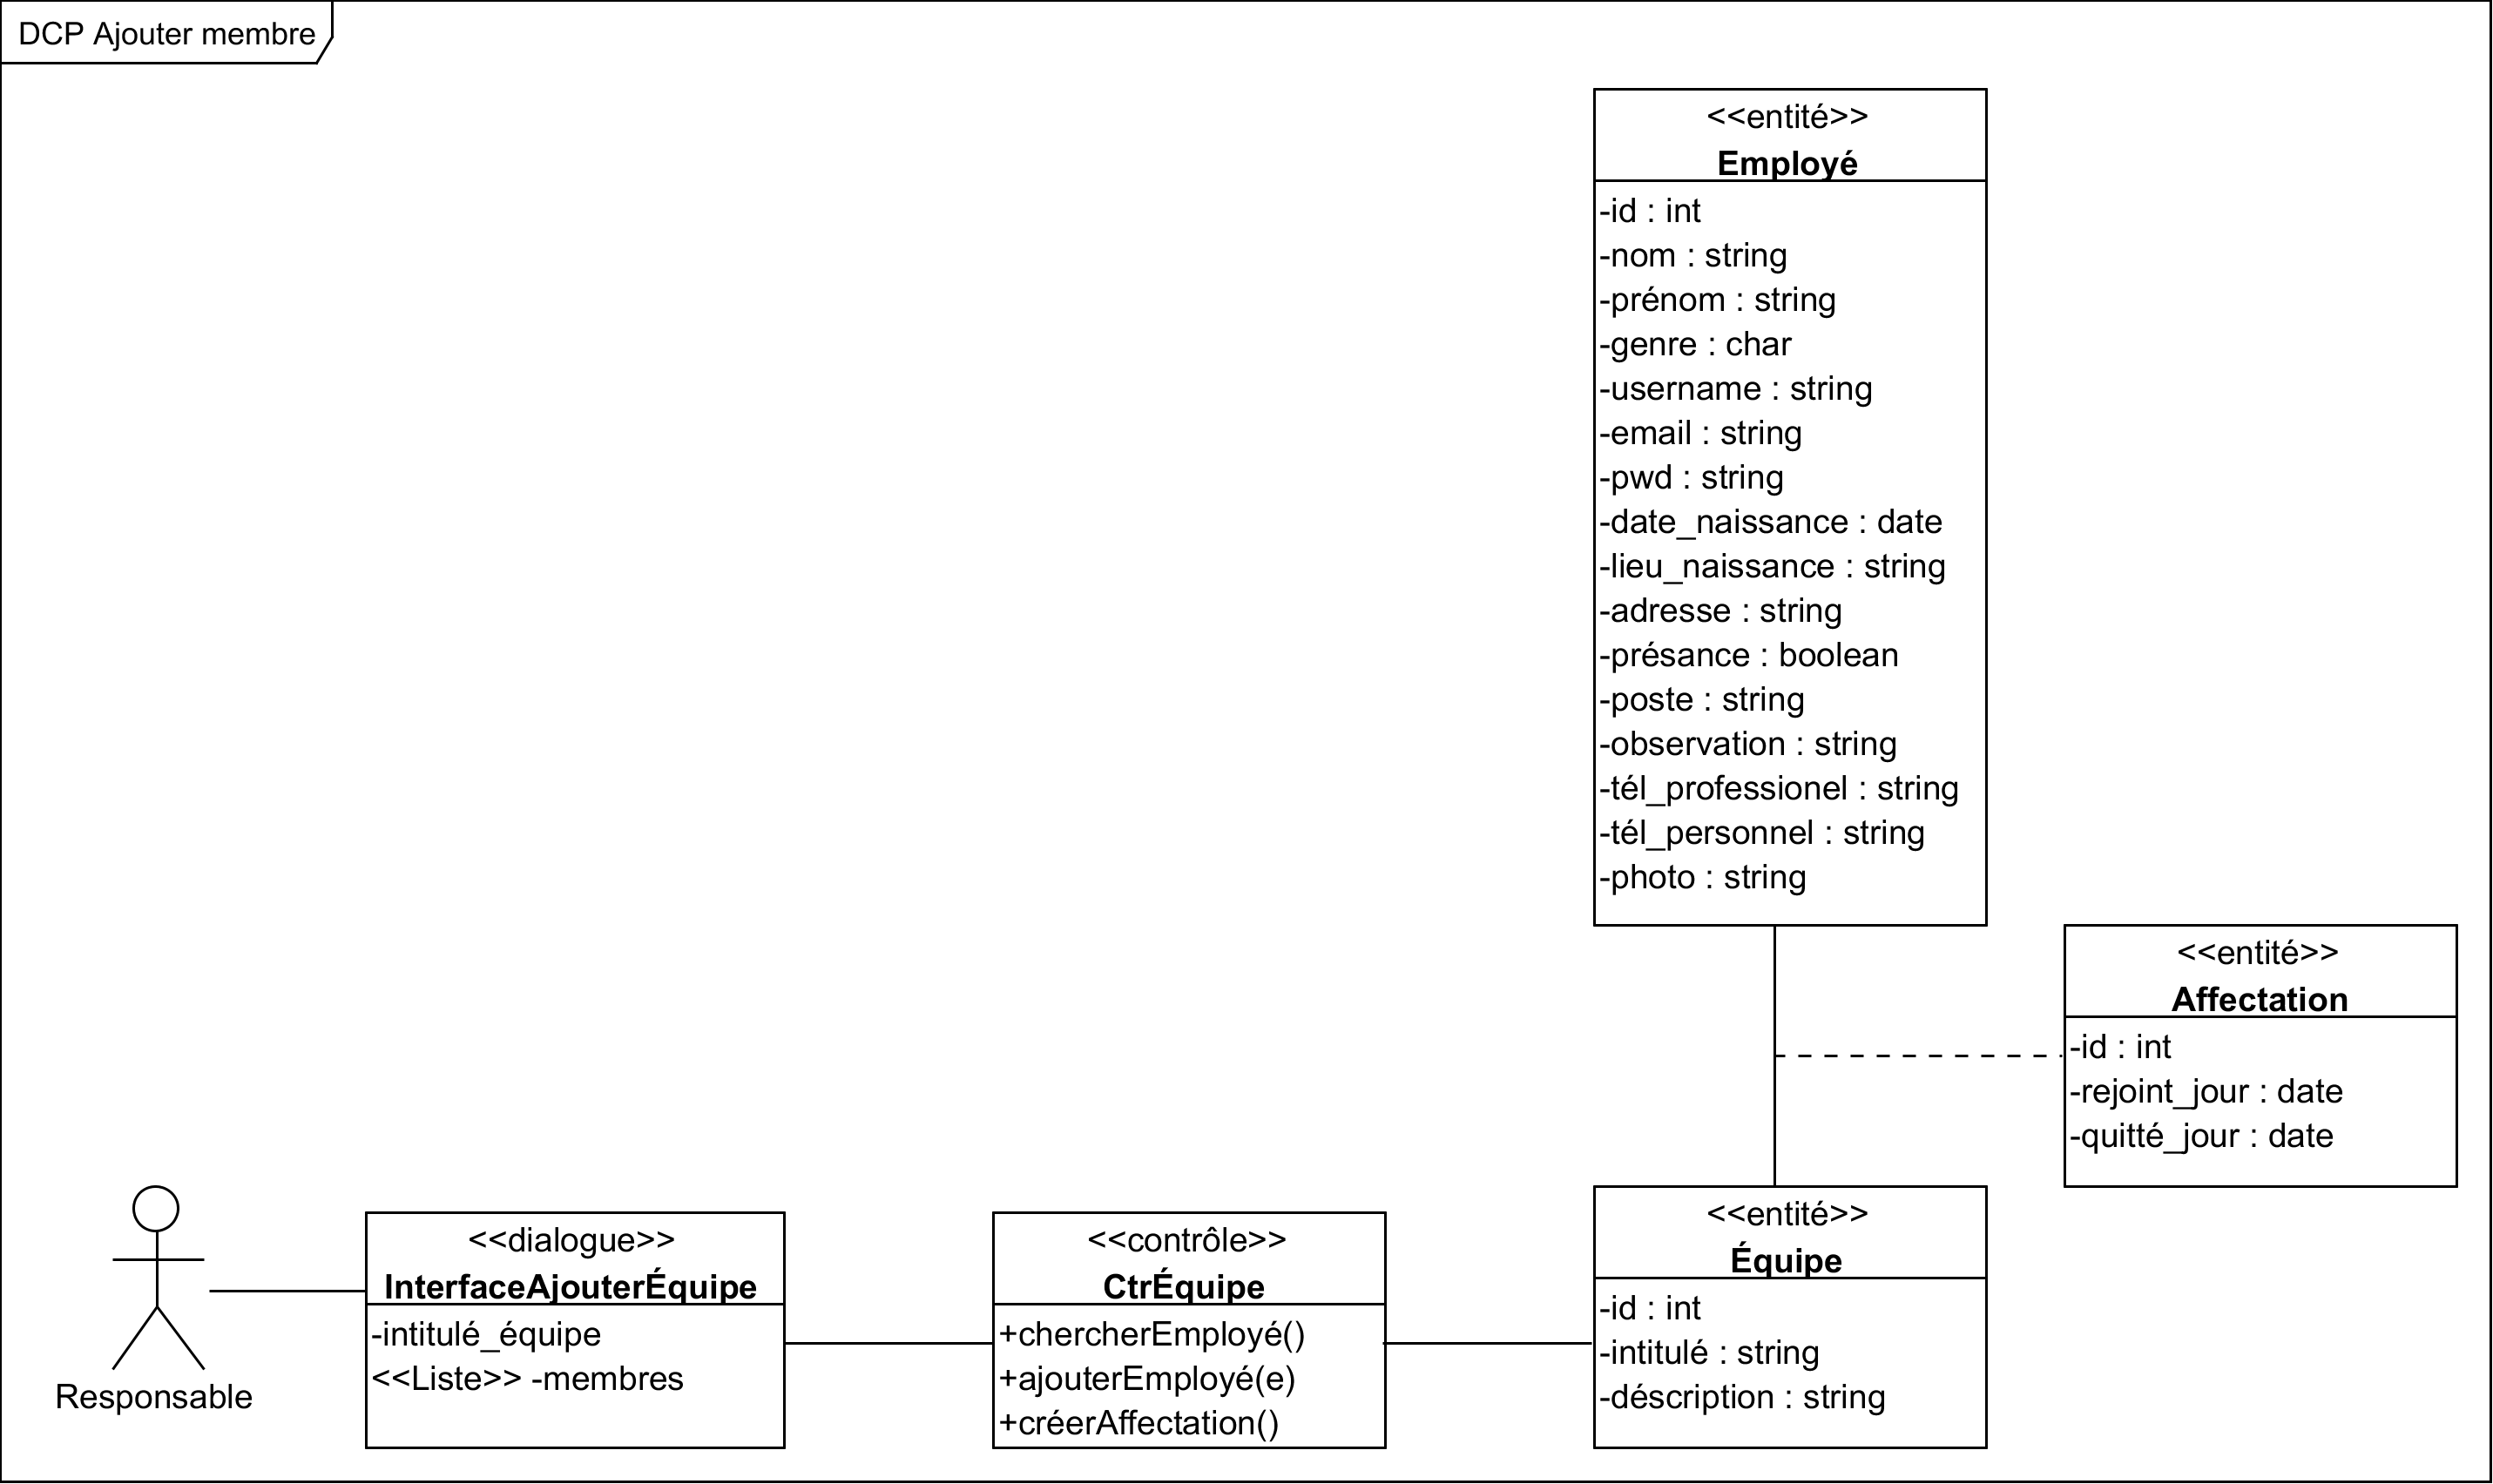
\includegraphics[scale=0.72]{images/DCP/DCP Ajouter membre.png}
    \caption{Diagrammes de classes participantes « Ajouter membre »}
    \label{fig30}
\end{figure}
            
\subsection*{Diagrammes de classes participantes du cas d'utilisation « Ajouter employé »}
L’administrateur à travers l’interface « InterfaceAjouterEmployé » peut ajouter
un employé en remplissant le formulaire. Après avoir validé, l’administrateur
devra ajouter l’empreinte de l’employé qui sera gérée par la classe
CtrEmpreinte.  Une fois enregistrée, la classe CtrEmployé récupèrera l’empreinte
pour finaliser l’enregistrement de l’employé. 

\clearpage

\begin{figure}[h!]
    \centering
    \includegraphics[scale=0.7]{images/DCP/DCP Ajouter employé.png}
    \caption{Diagrammes de classes participantes « Ajouter employé »}
    \label{fig31}
\end{figure}
        
\subsection*{Diagrammes de classes participantes du cas d'utilisation « Consulter profil d'un employé »}
L’interface « InterfaceConsulterProfilEmployé » permet au responsable de 
consulter le profil d’un employé où il aura accès à toutes ses informations. Il 
pourra aussi à partir de cette interface accéder à l’interface de modification
du profil et du planning de l’employé. Quant à la classe CtrEmployé, elle permet 
de récupérer l’employé sélectionner. 

\begin{figure}[h!]
    \centering
    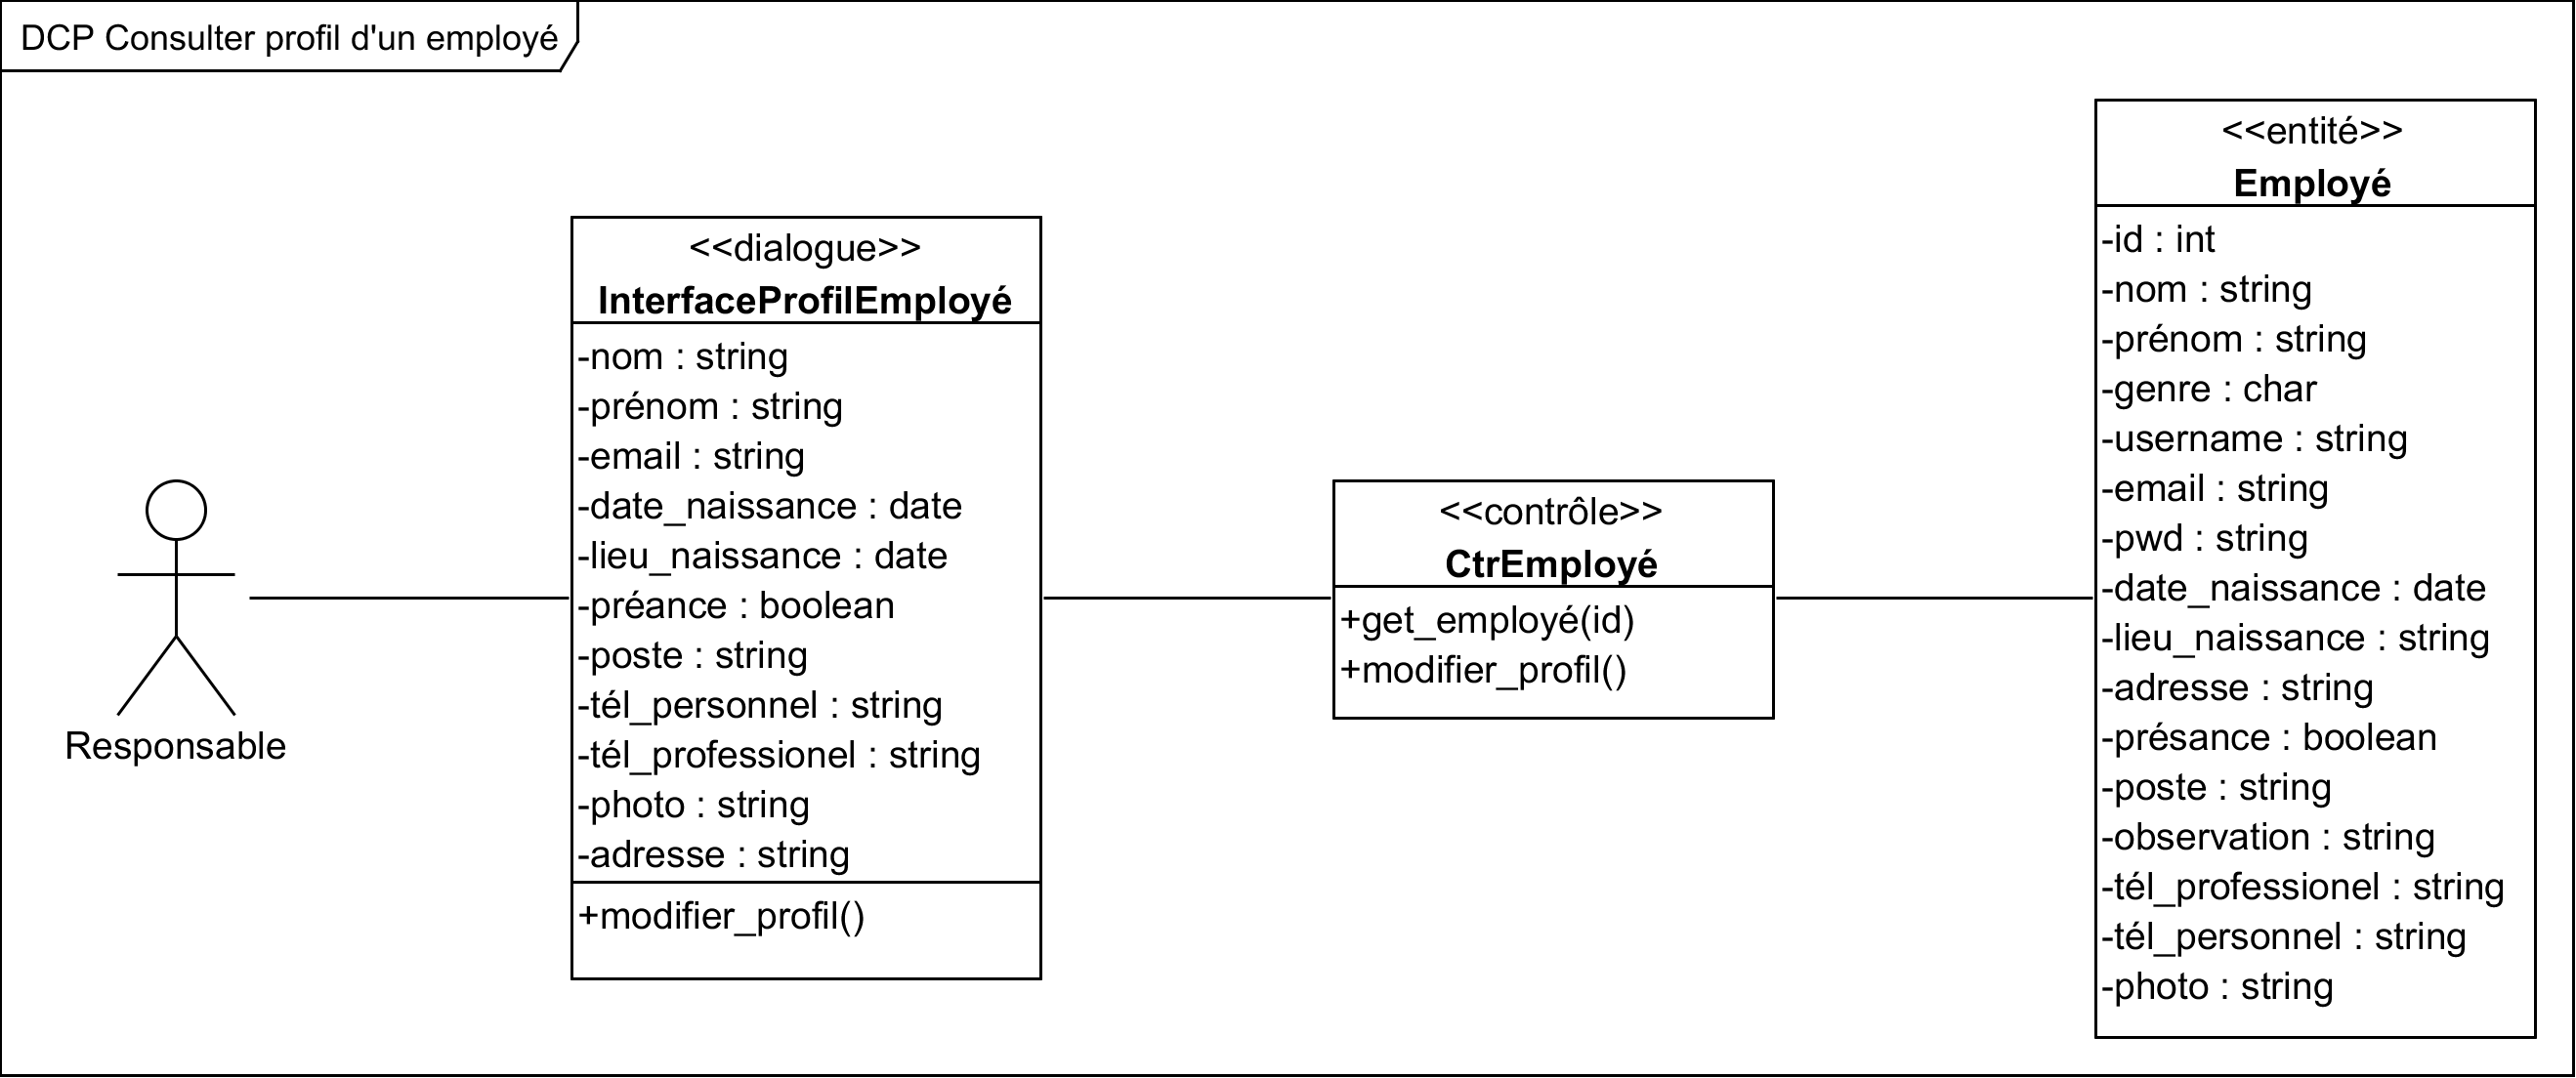
\includegraphics[scale=0.72]{images/DCP/DCP_consulter_profil_d'un_employe.png}
    \caption{Diagrammes de classes participantes « Consulter profil employé »}
    \label{fig32}
\end{figure}
             
\section{Diagrammes de séquence}
L’objectif du diagramme de séquence est de représenter les interactions entre 
objets en indiquant la chronologie des échanges. Cette représentation peut se 
réaliser par cas d’utilisation en considérant les différents scénarios 
associés.\cite{9} 
    
Dans cette partie, nous allons détailler les diagrammes de séquence système 
élaborés dans le chapitre 2, en remplaçant le système vu comme une boîte 
noire par un ensemble d’objets de classes différentes tout en respectant 
les règles suivantes:

\begin{itemize}
        \item[\textbullet] Les acteurs ne peuvent interagir (envoyer des messages) 
            qu’avec les dialogues.
        \item[\textbullet] Les dialogues peuvent interagir avec les contrôles. 
        \item[\textbullet] Les contrôles peuvent interagir avec les dialogues, les 
            entités, ou d’autres contrôles.
        \item[\textbullet] Les entités ne peuvent interagir qu’entre elles.             
\end{itemize}

Le formalisme est donné dans l’exemple type présenté à la figure \ref{fig33}\\

\begin{figure}[h!]
    \centering                 
    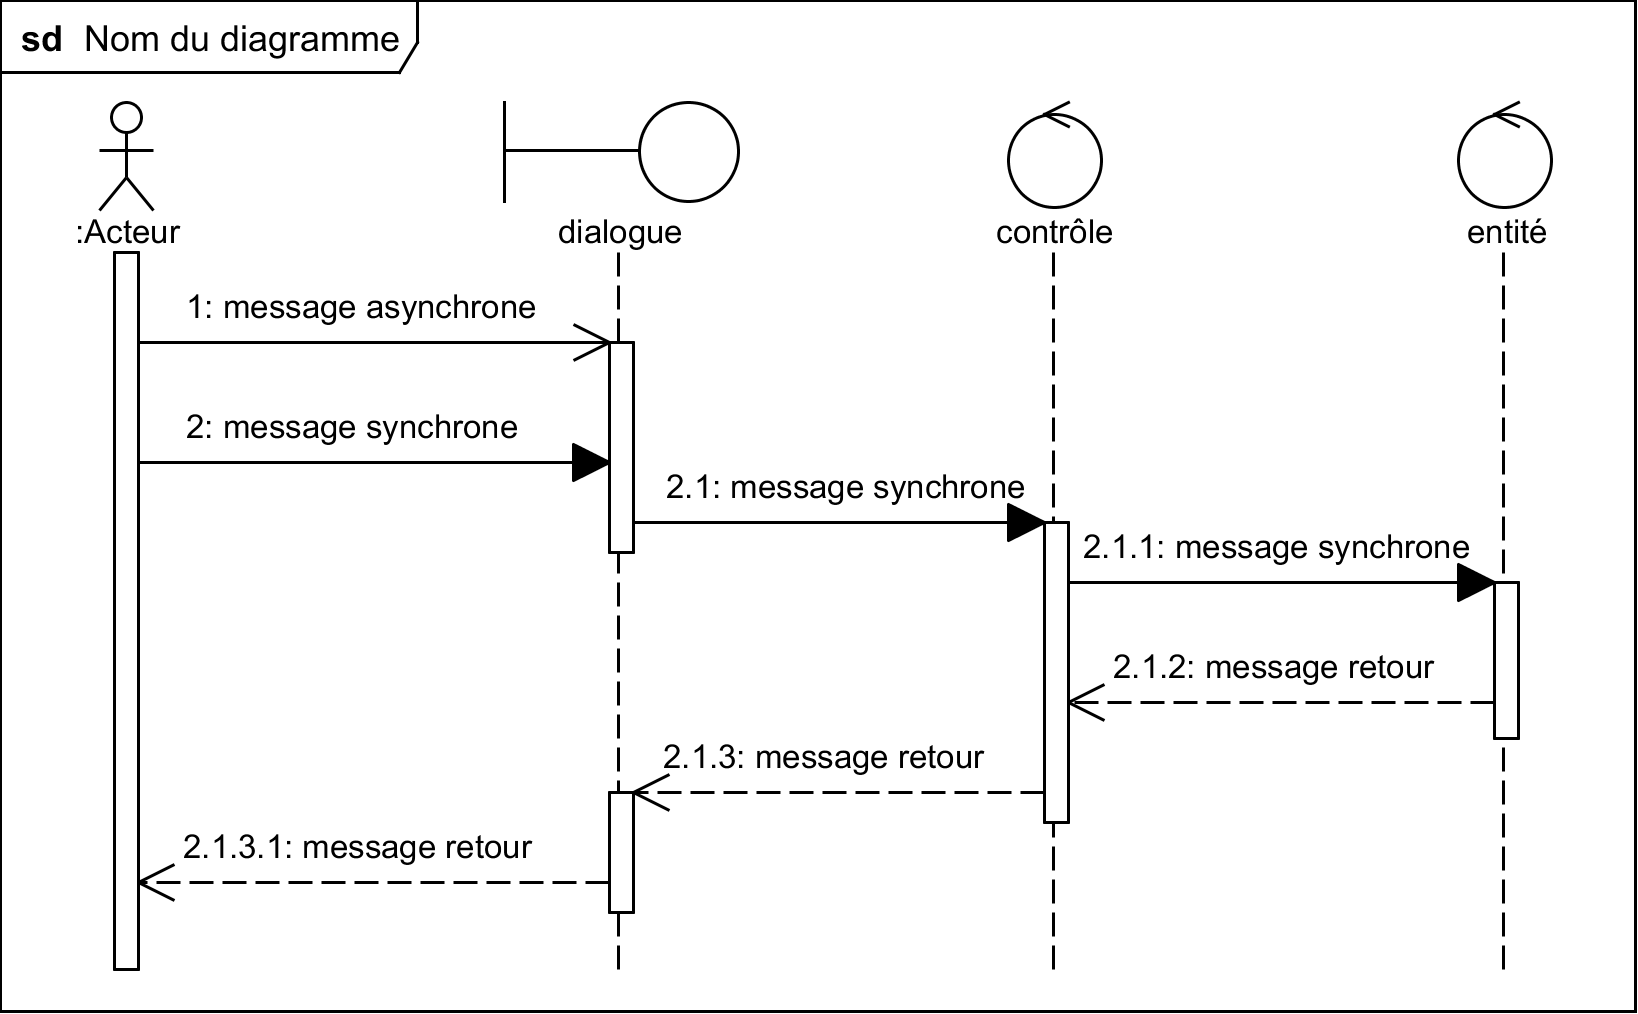
\includegraphics[scale=1.23]{images/exemple ds.png}
    \caption{Formalisme du diagramme de séquence}
    \label{fig33}
\end{figure}

\clearpage
    
\subsection*{Diagramme d'interaction du cas d'utilisation « Se pointer »}
Avant chaque entrée ou sortie de l’entreprise, l’employé doit se pointer avec son 
empreinte digitale afin que la pointeuse l’identifie. Après une courte 
vérification, si l’empreinte n’est pas reconnue aucune LED ne s’allume, par 
contre si la pointeuse la reconnait, elle signale au contrôle CtrEmployé qui 
récupère son identifiant, puis délègue au contrôle CtrShift la recherche de son 
dernier pointage et la vérification du type de pointage. Une fois effectué, le 
contrôle CtrEmployé déclenche l’enregistrement du pointage, si le type de 
pointage est une sortie alors le contrôle CtrShift insérera l’heure de sortie 
dans le dernier pointage, si c’est une entrée alors un nouveau pointage est 
créé avec l’heure d’entrée et l’identifiant de l’employé.

\begin{figure}[h!]
    \centering
    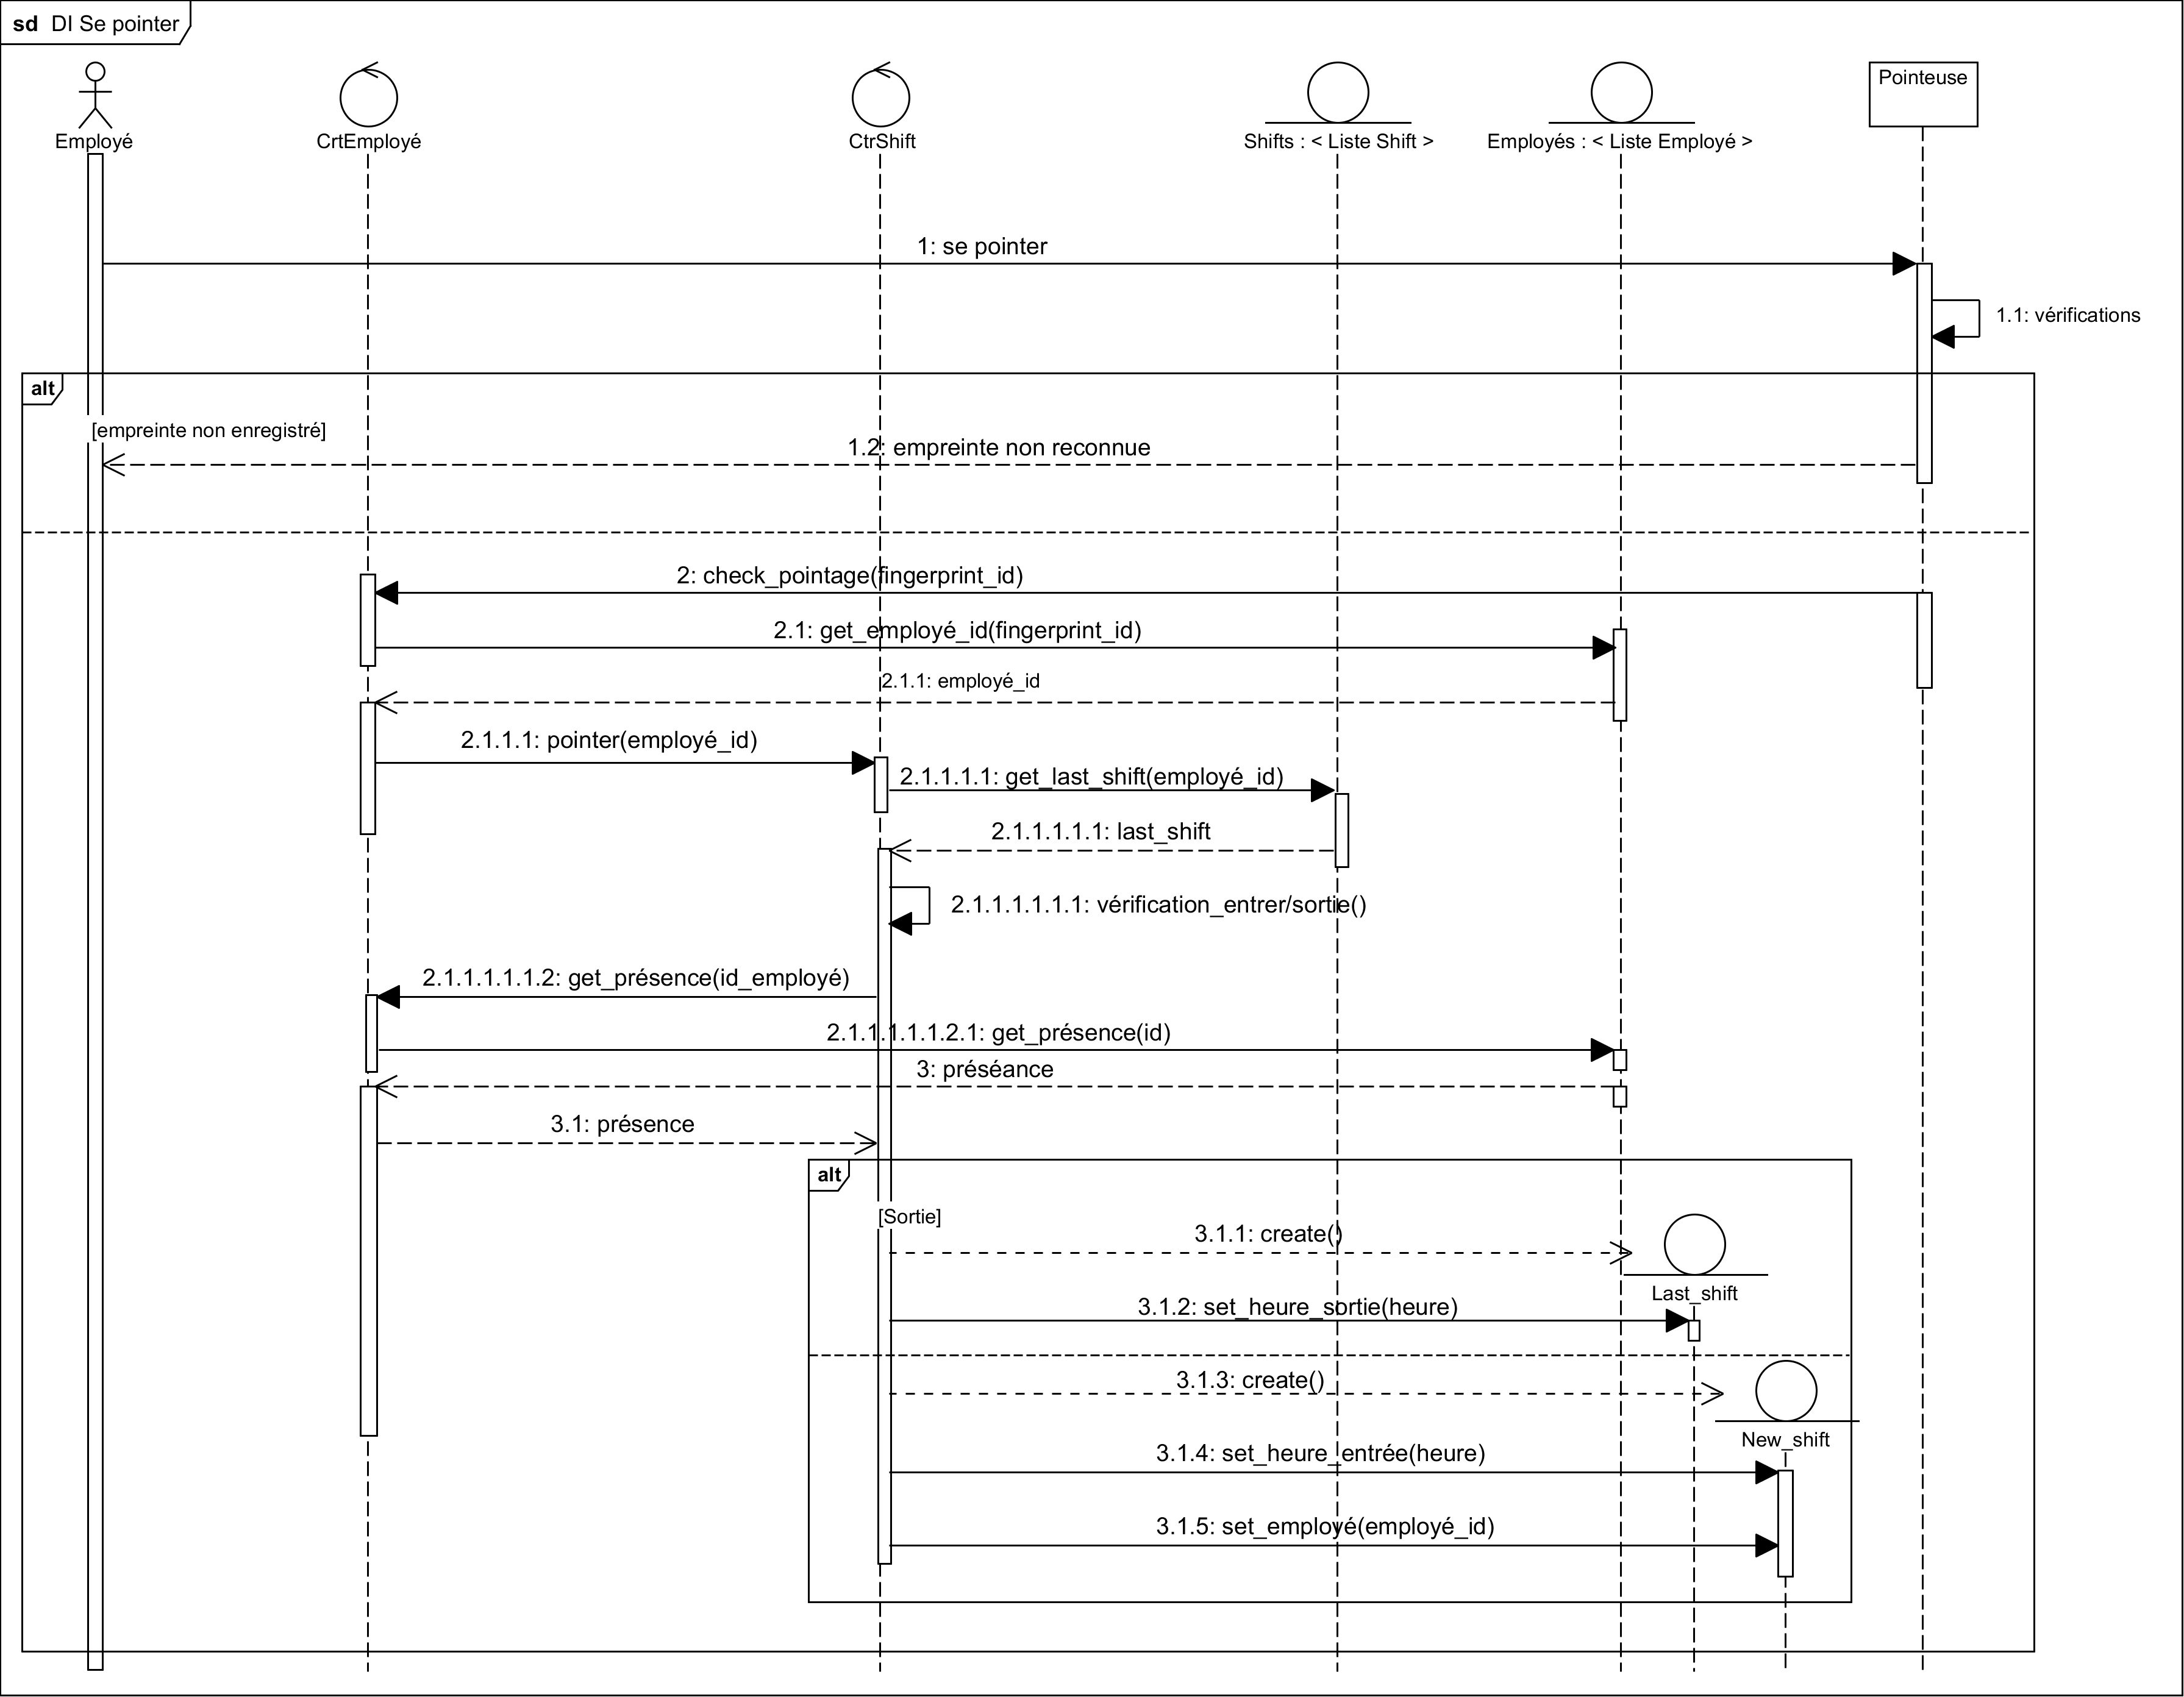
\includegraphics[scale=0.56]{images/DS/DI Se pointer.png}
    \caption{Diagramme d'interaction « Se pointer »}
    \label{fig34}
\end{figure}
        
\clearpage
    
\subsection*{Diagramme d'interaction du cas d'utilisation « Consulter mon profil »}
Une fois authentifié, l’employé peut consulter son profil à travers n’importe 
quelle interface, il est redirigé vers l’interface MonProfil qui délègue la 
recherche avec l’identifiant au contrôle CtrEmployé. Une fois la recherche 
effectuée, les informations sont affichées. Il pourra aussi à travers cette 
interface modifier son profil. Une fois les informations saisies, il doit 
valider ce qui déclenchera une vérification, si les informations saisies sont 
correctes les modifications seront enregistrées. Dans le cas contraire, un 
message d’erreur sera affiché.

\begin{figure}[h!]
    \centering
    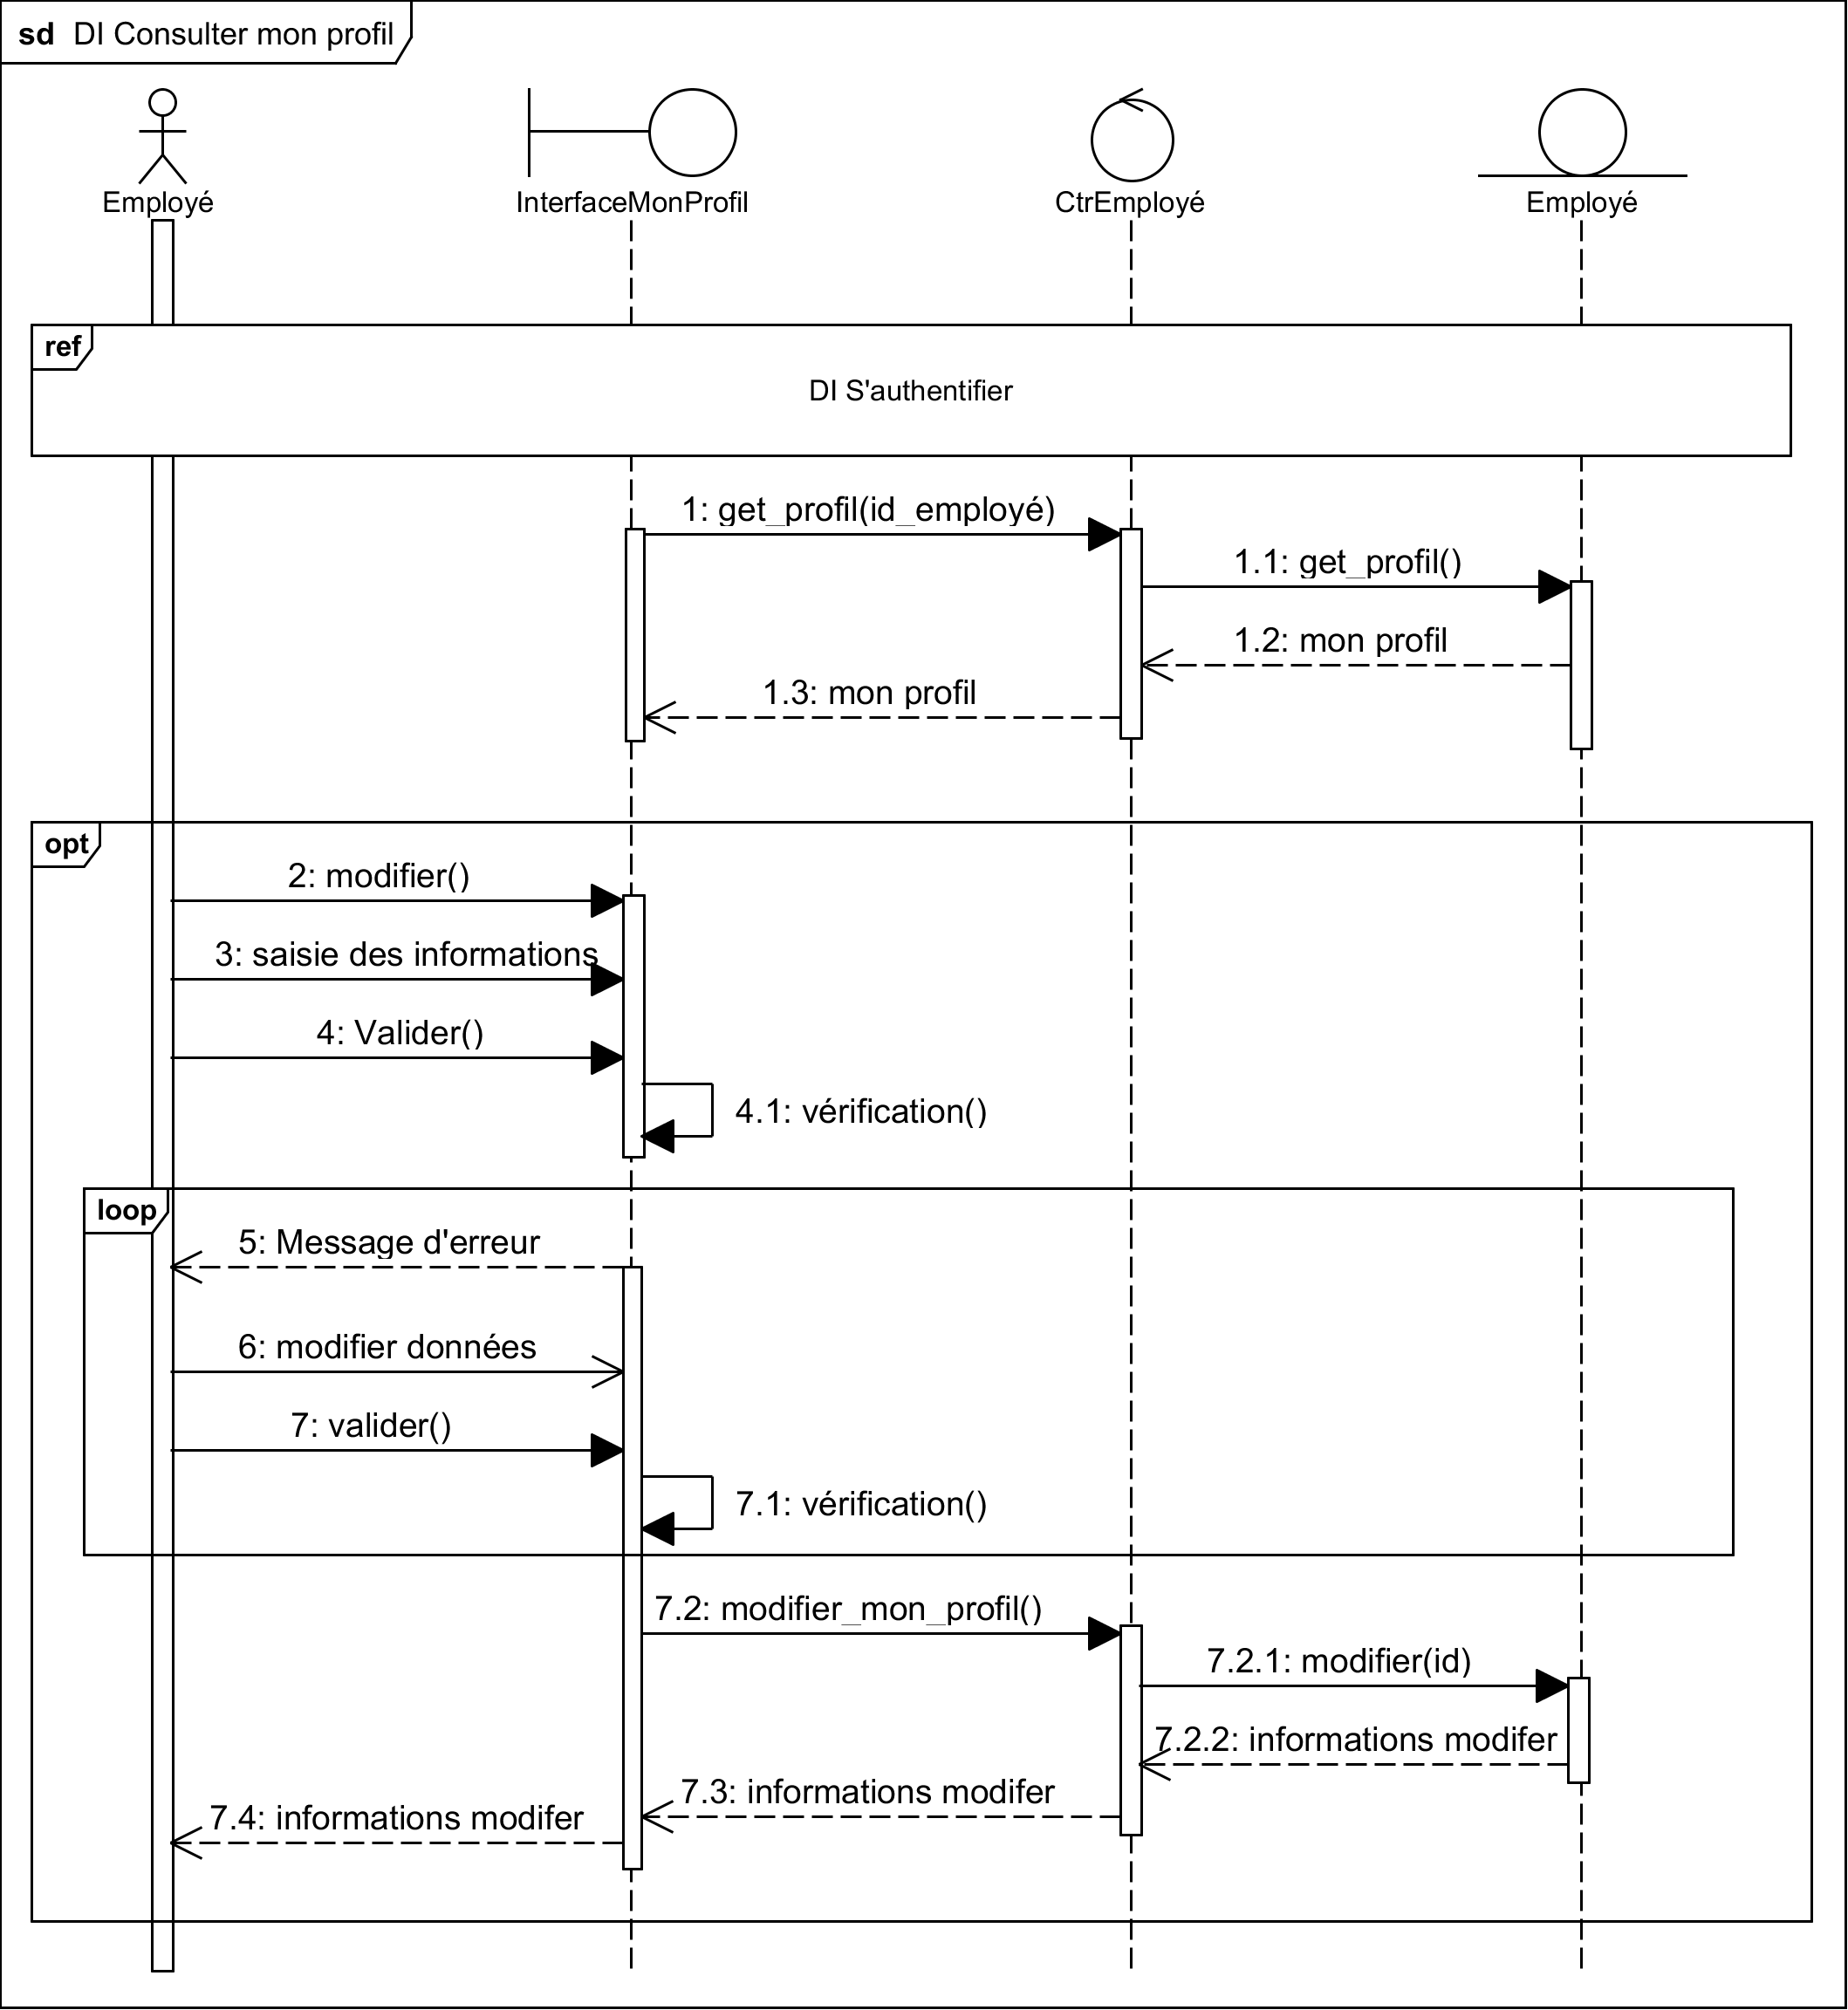
\includegraphics[scale=0.86]{images/DS/consulter_mon_profile}
    \caption{Diagramme d'interaction « Consulter mon profil »}
    \label{fig35}
\end{figure}

\clearpage
    
\subsection*{Diagramme d'interaction du cas d'utilisation « Consulter ma fiche de pointage »}
L’employé devra s’authentifier pour consulter sa fiche de pointage. L’interface 
InterfaceMaFicheDePointage déléguera la recherche de la liste des derniers 
pointages au contrôle CtrShift qui seront affichés par semaine. L’employé aura 
aussi la possibilité de les afficher par mois, ainsi que de faire une recherche 
par période. 
        
\begin{figure}[h!]
    \centering
    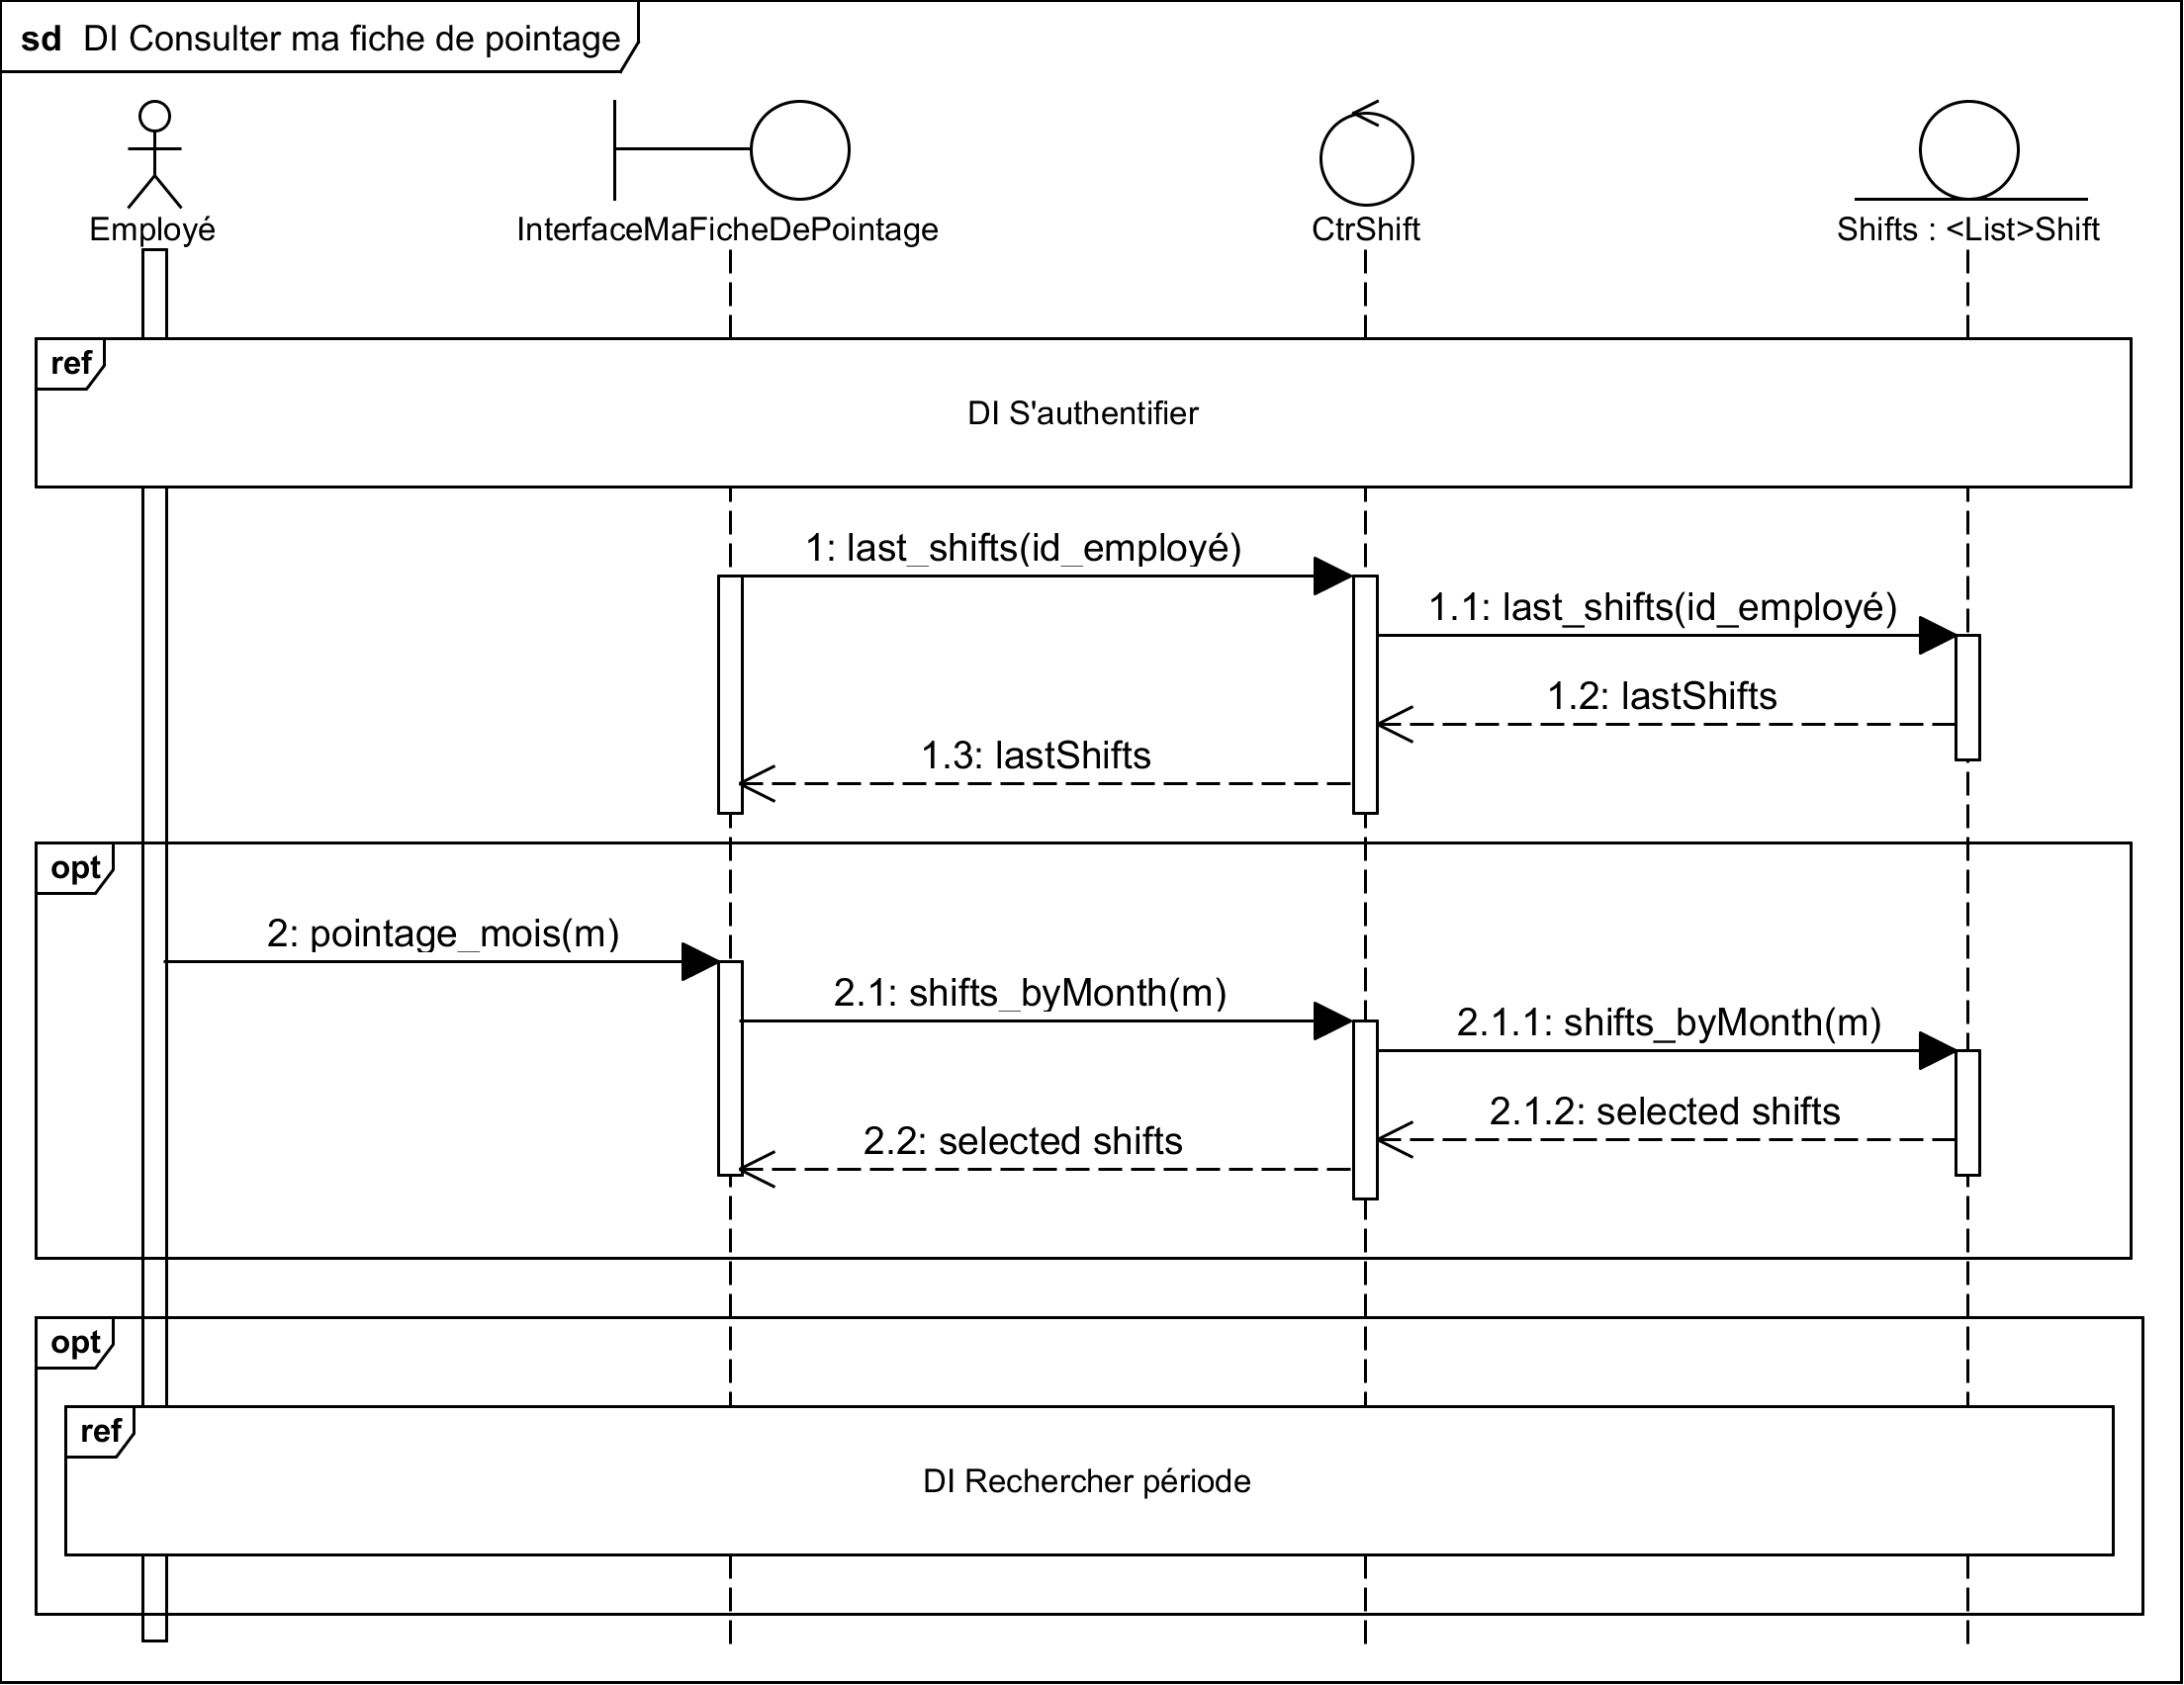
\includegraphics[scale=0.86]{images/DS/DI Consulter ma fiche de pointage.png}
    \caption{Diagramme d'interaction « Consulter ma fiche de pointage »}
    \label{fig36}
\end{figure}    
        
\subsection*{Diagramme d'interaction du cas d'utilisation « Consulter tableau de bord manager »}
Une fois authentifié, le manager est redirigé vers son tableau de bord. En 
premier lieu son espace personnel sera affiché, il pourra sélectionner l’espace 
manager, 3 contrôleurs seront nécessaires, le contrôle CtrEmployé pour récupérer 
la liste de ses collaborateurs, le contrôle CtrEquipe pour récupérer la liste 
des équipes du manager, et le dernier contrôle CtrSHift pour récupérer la liste 
des pointages de ses collaborateurs.

\clearpage

\begin{figure}[h!]
    \centering
    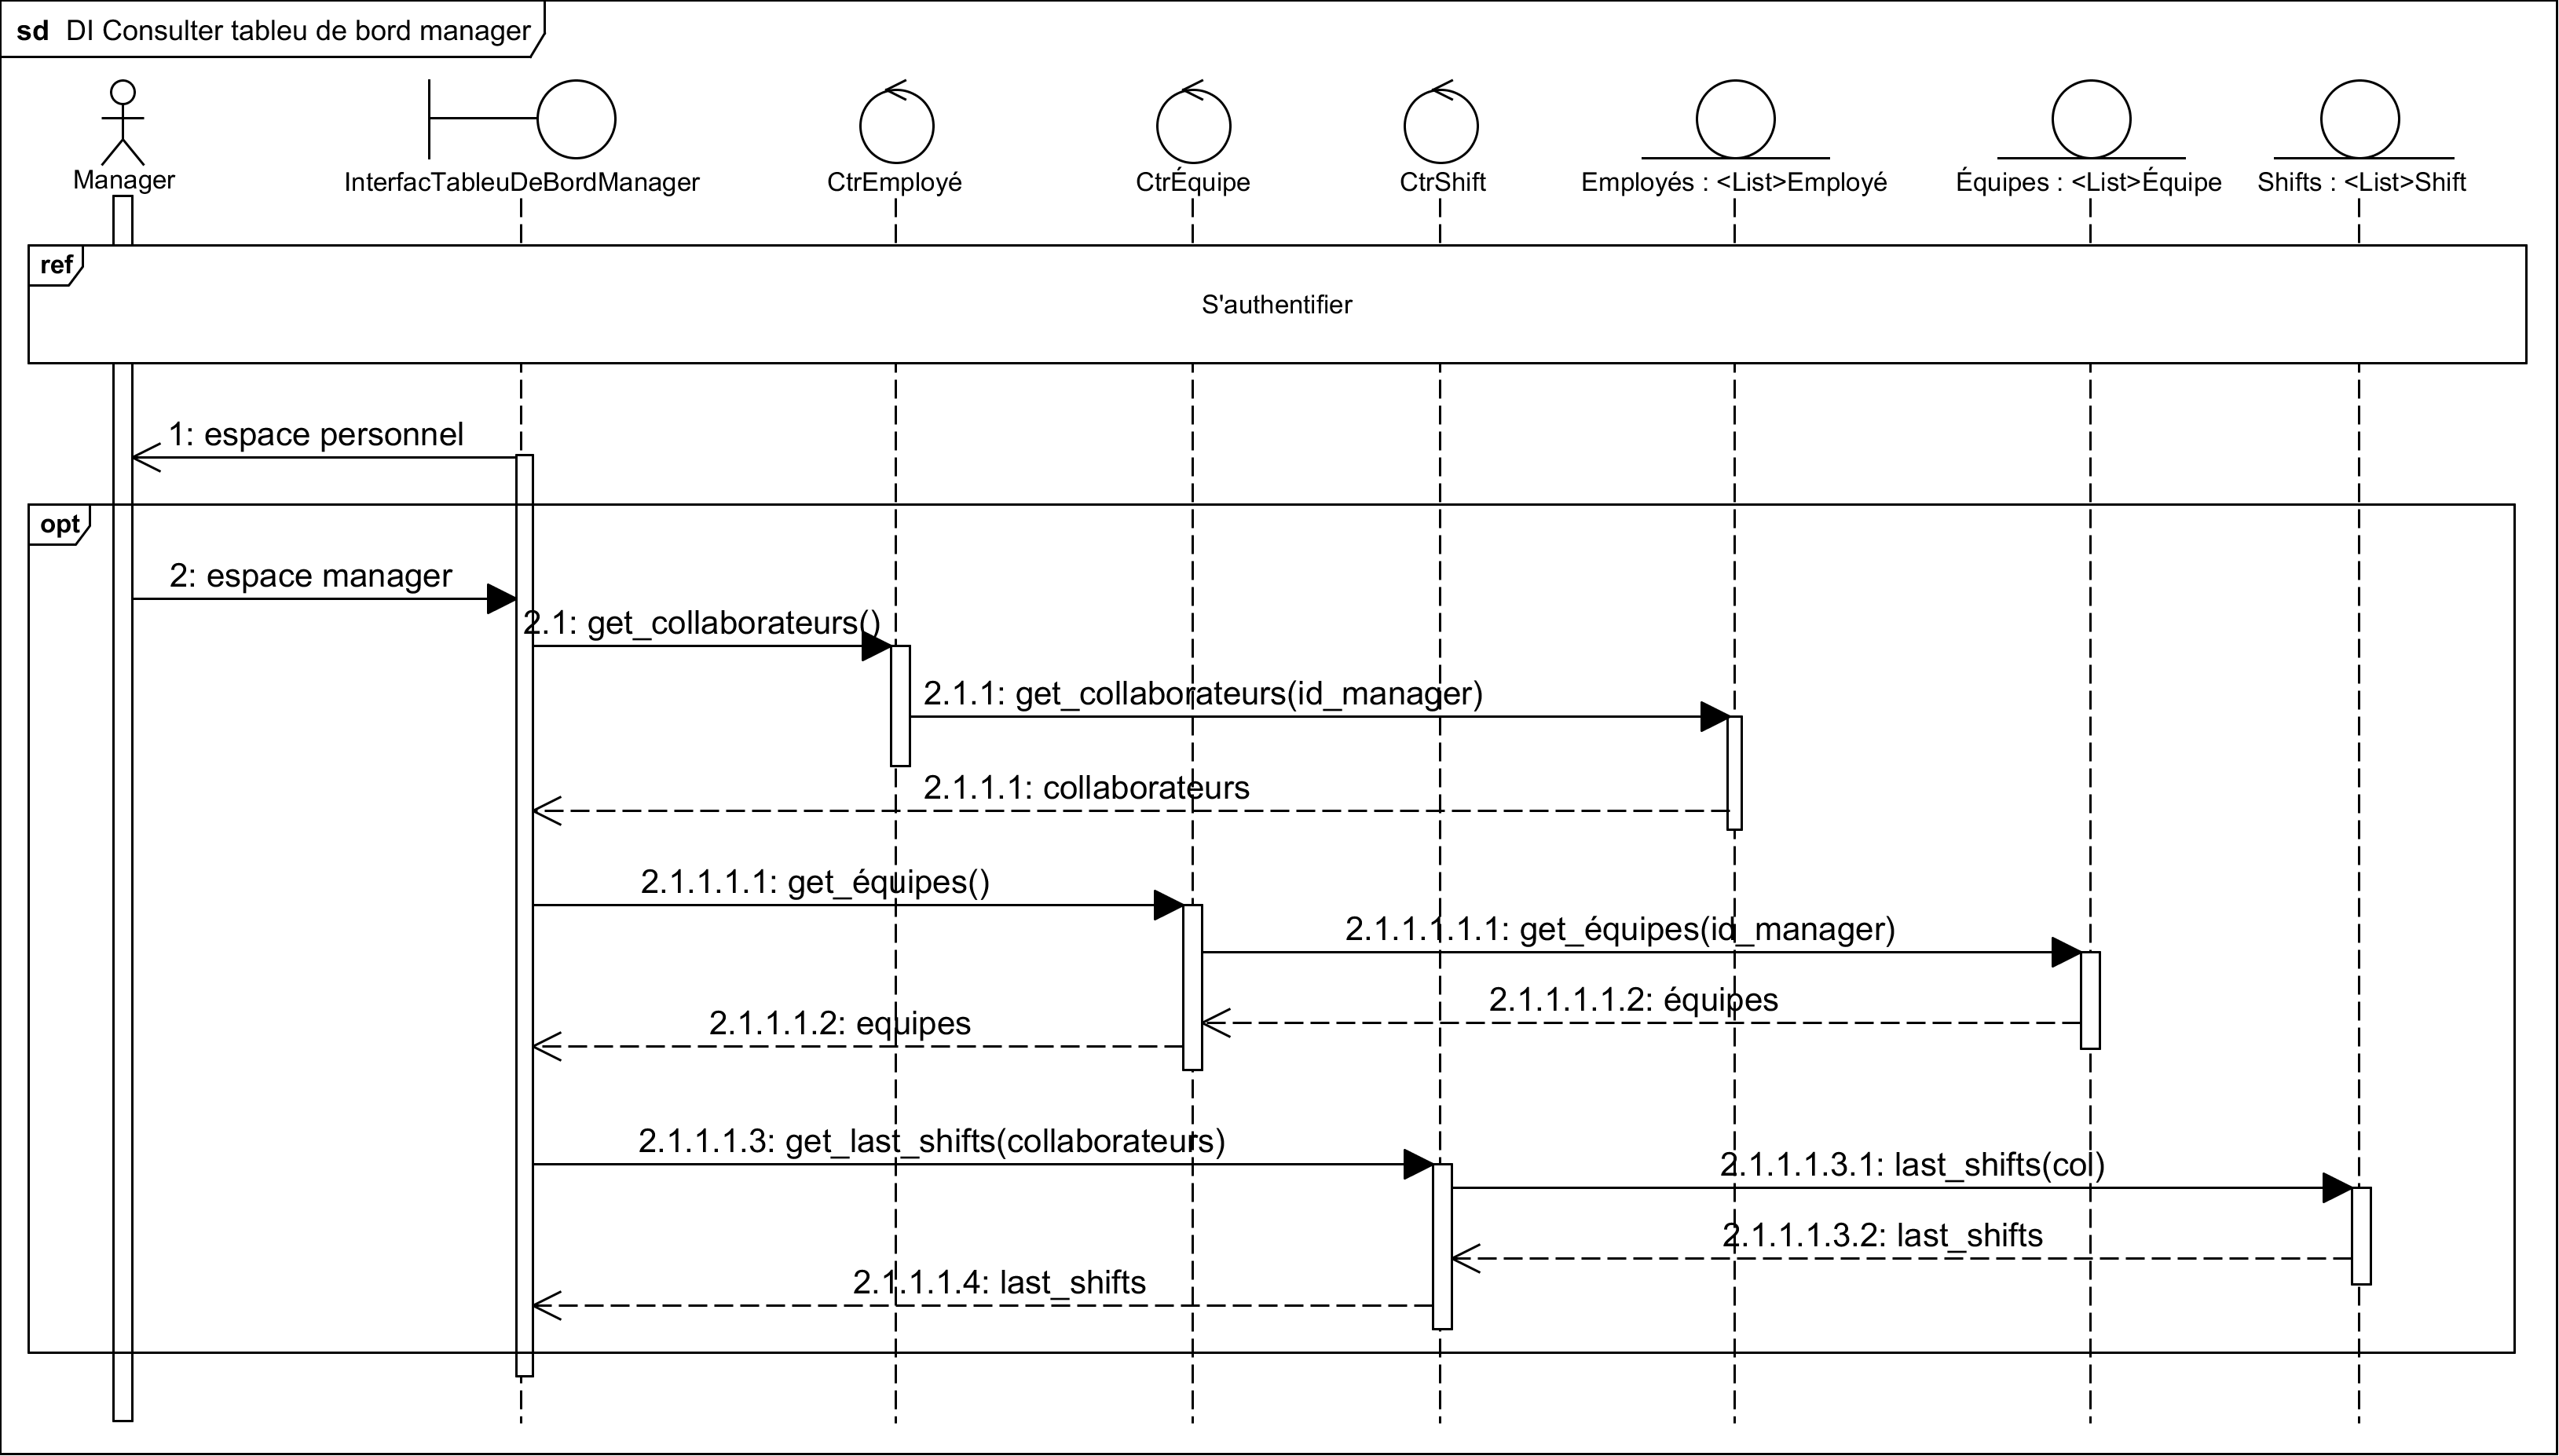
\includegraphics[angle=90,scale=0.65]{images/DS/DI Consulter tableu de bord manager.png}
	\caption{Diagramme d'interaction « Consulter tableau de bord manager »}
    \label{fig37}
\end{figure}
        
\subsection*{Diagramme d'interaction du cas d'utilisation « Ajouter équipe »}
L’acteur pourra ajouter une équipe. Après avoir saisi les informations et
sélectionné un manager, une vérification est effectuée. Si aucune erreur n’est
détectée il pourra l’enregistrer, le contrôle CtrEquipe s’occupera de la
création et il déléguera la recherche du manager au contrôle CtrManager, une
fois terminée, l’interface InterfaceAjouterEquipe est détruite et l’acteur sera
redirigé vers l’interface InterfaceGérerEquipe, où il pourra affecter des
membres.

\clearpage

\begin{figure}[h!]
    \centering
    \includegraphics[scale=0.74]{images/DS/DI Ajouter une équipe.png}
    \caption{Diagramme d'interaction « Ajouter équipe »}
    \label{fig38}
\end{figure}

\subsection*{Diagramme d'interaction du cas d'utilisation « Ajouter planning »}
L’acteur aura la possibilité d’ajouter un planning. Pour ce, il doit saisir les
horaires de travail de la semaine ainsi que l’intitulé et la description du
planning.  Après la validation, une vérification des informations sera
effectuée. Si les données sont invalides un message d’erreur sera affiché et
l’acteur devra les corriger. Si les informations sont valides, le contrôle
CtrPlanning vérifiera si aucun planning n’existe avec l’intitulé saisi afin de
valider l’ajout du planning. Une fois terminé, l’acteur pourra affecter un
planning aux employés.

\clearpage

\begin{figure}[h!]
    \centering
    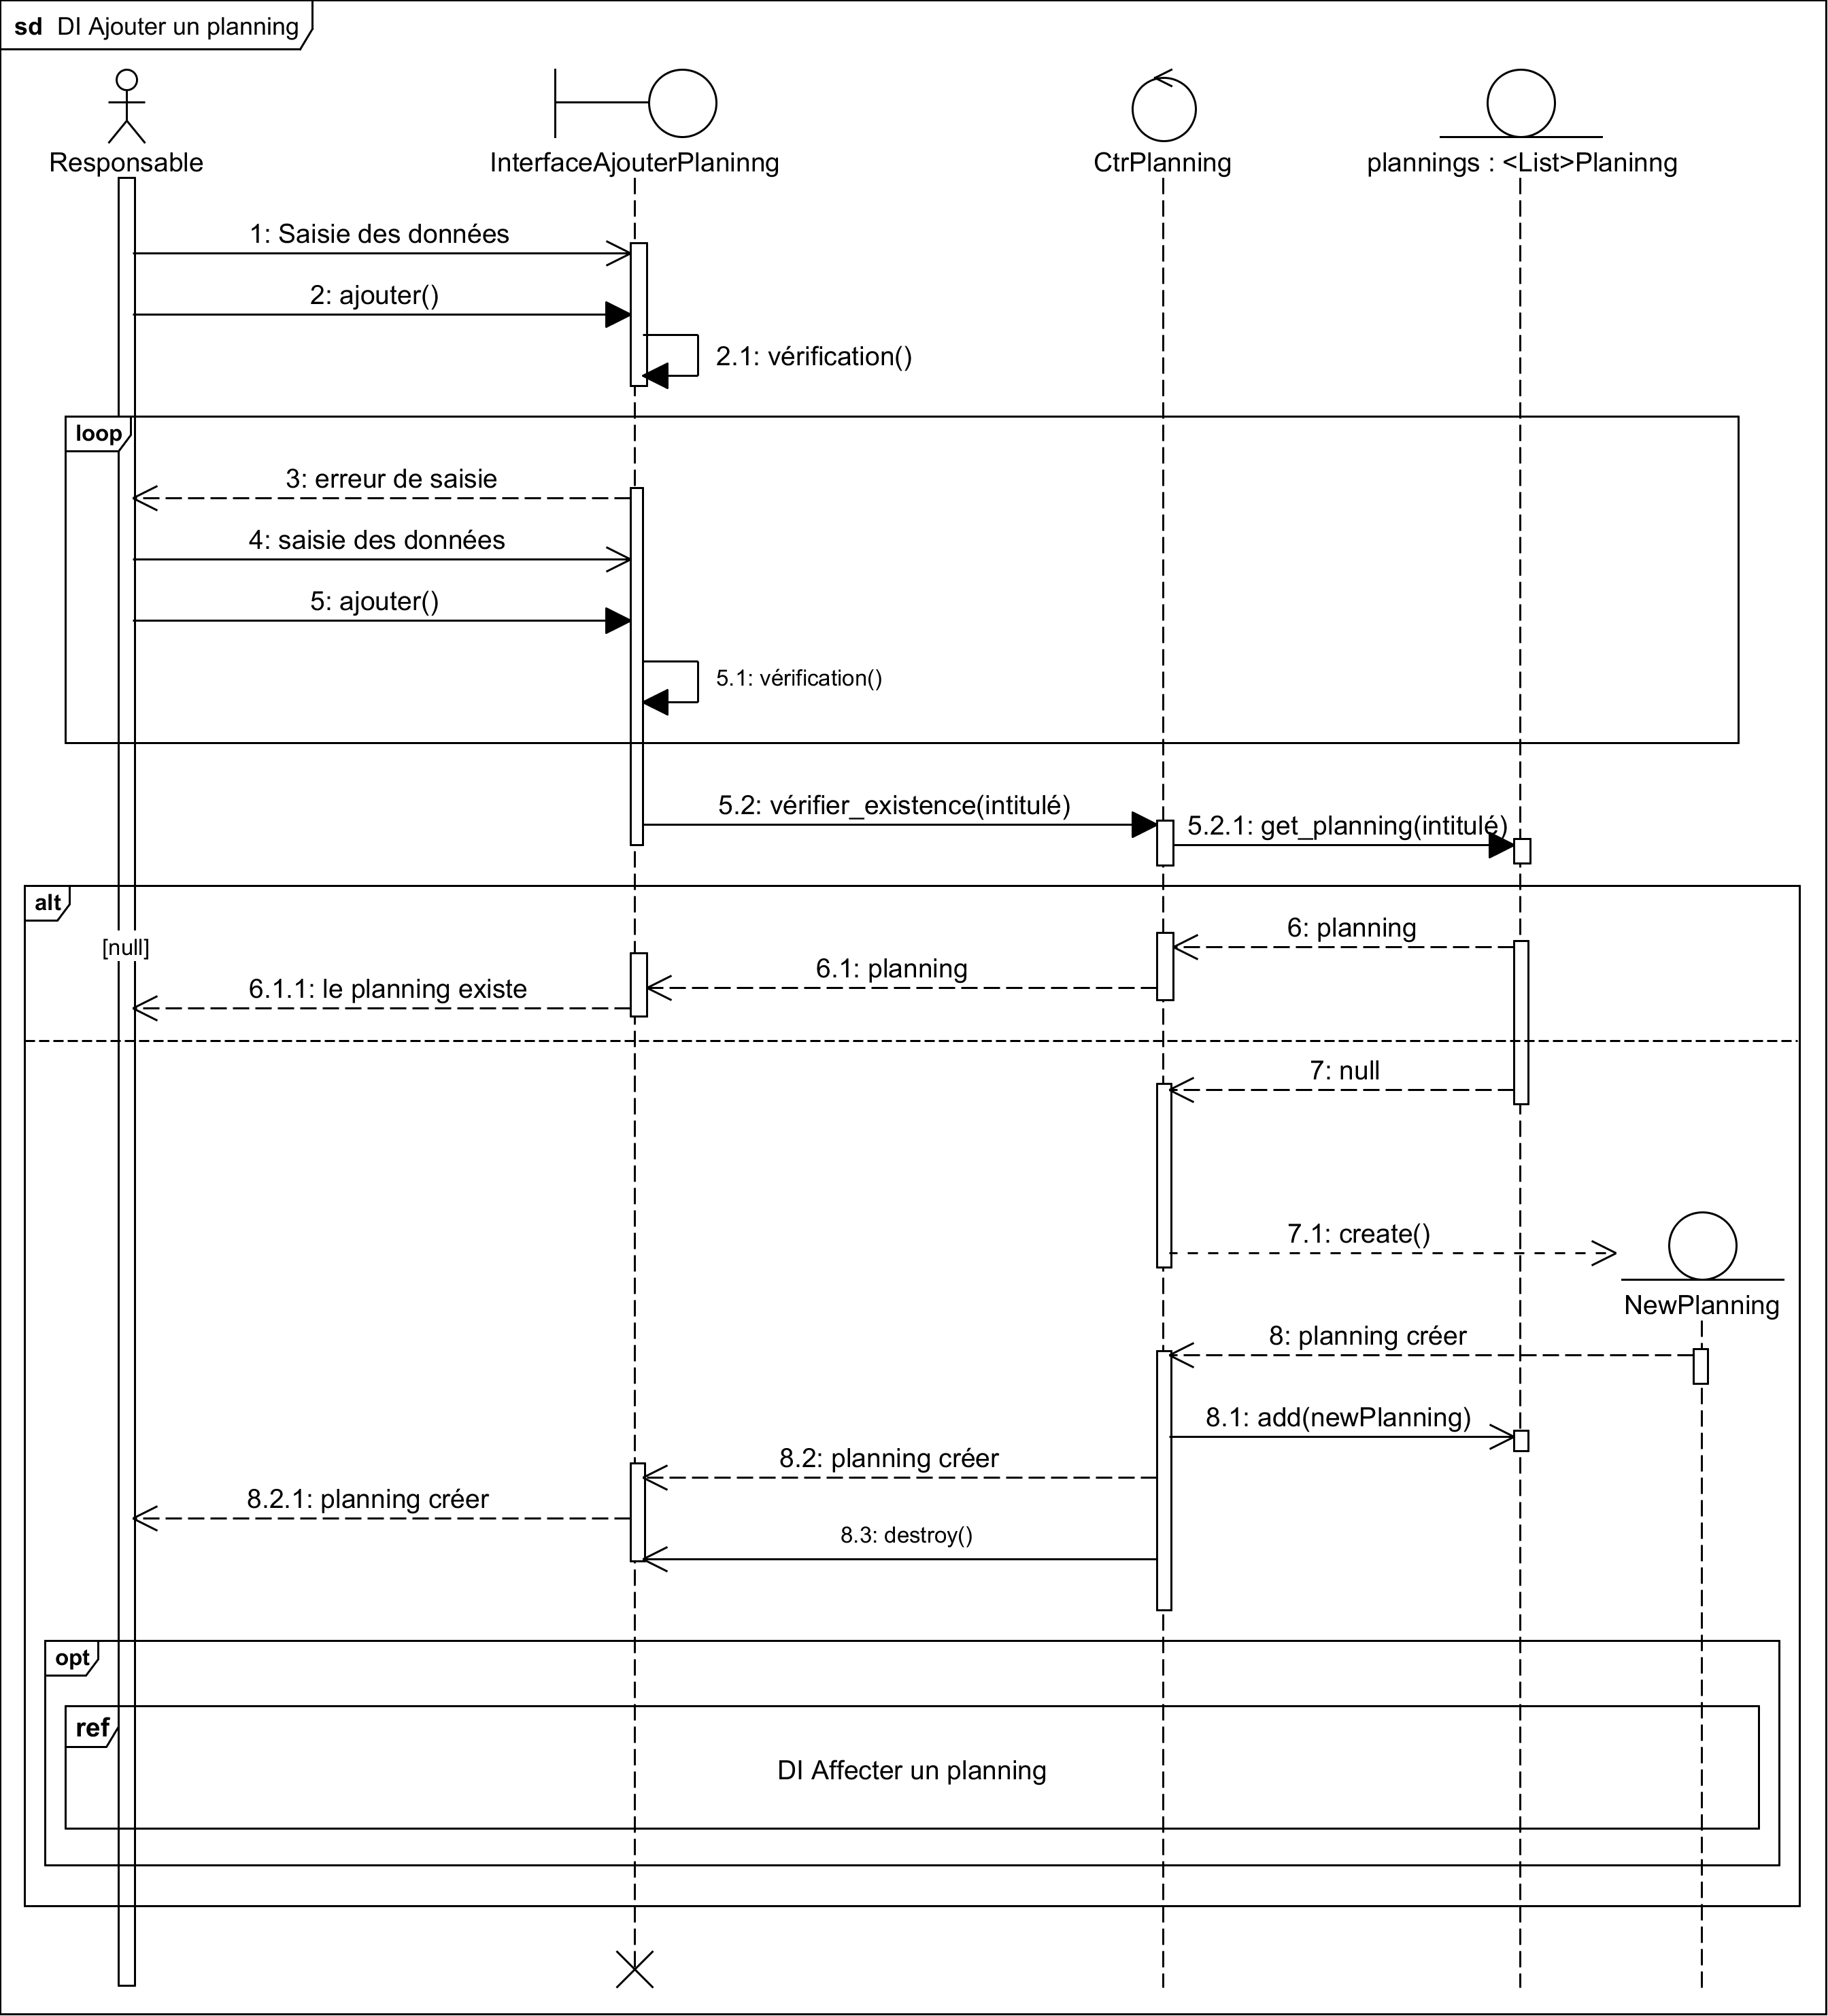
\includegraphics[scale=0.74]{images/DS/DI Ajouter un planning.png}
    \caption{Diagramme d'interaction « Ajouter planning »}
    \label{fig39}
\end{figure}
        
\subsection*{Diagramme d'interaction du cas d'utilisation « Ajouter membre »}
L’acteur aura la possibilité d’ajouter un membre à une équipe, il devra 
effectuer une recherche qui lui permettra à travers l’interface 
InterfaceAjouterMembre d’affecter un employé s’il existe à une équipe. Une fois 
terminé, le contrôle CtrEmployé retournera un message de confirmation.

\begin{figure}[h!]
    \centering
    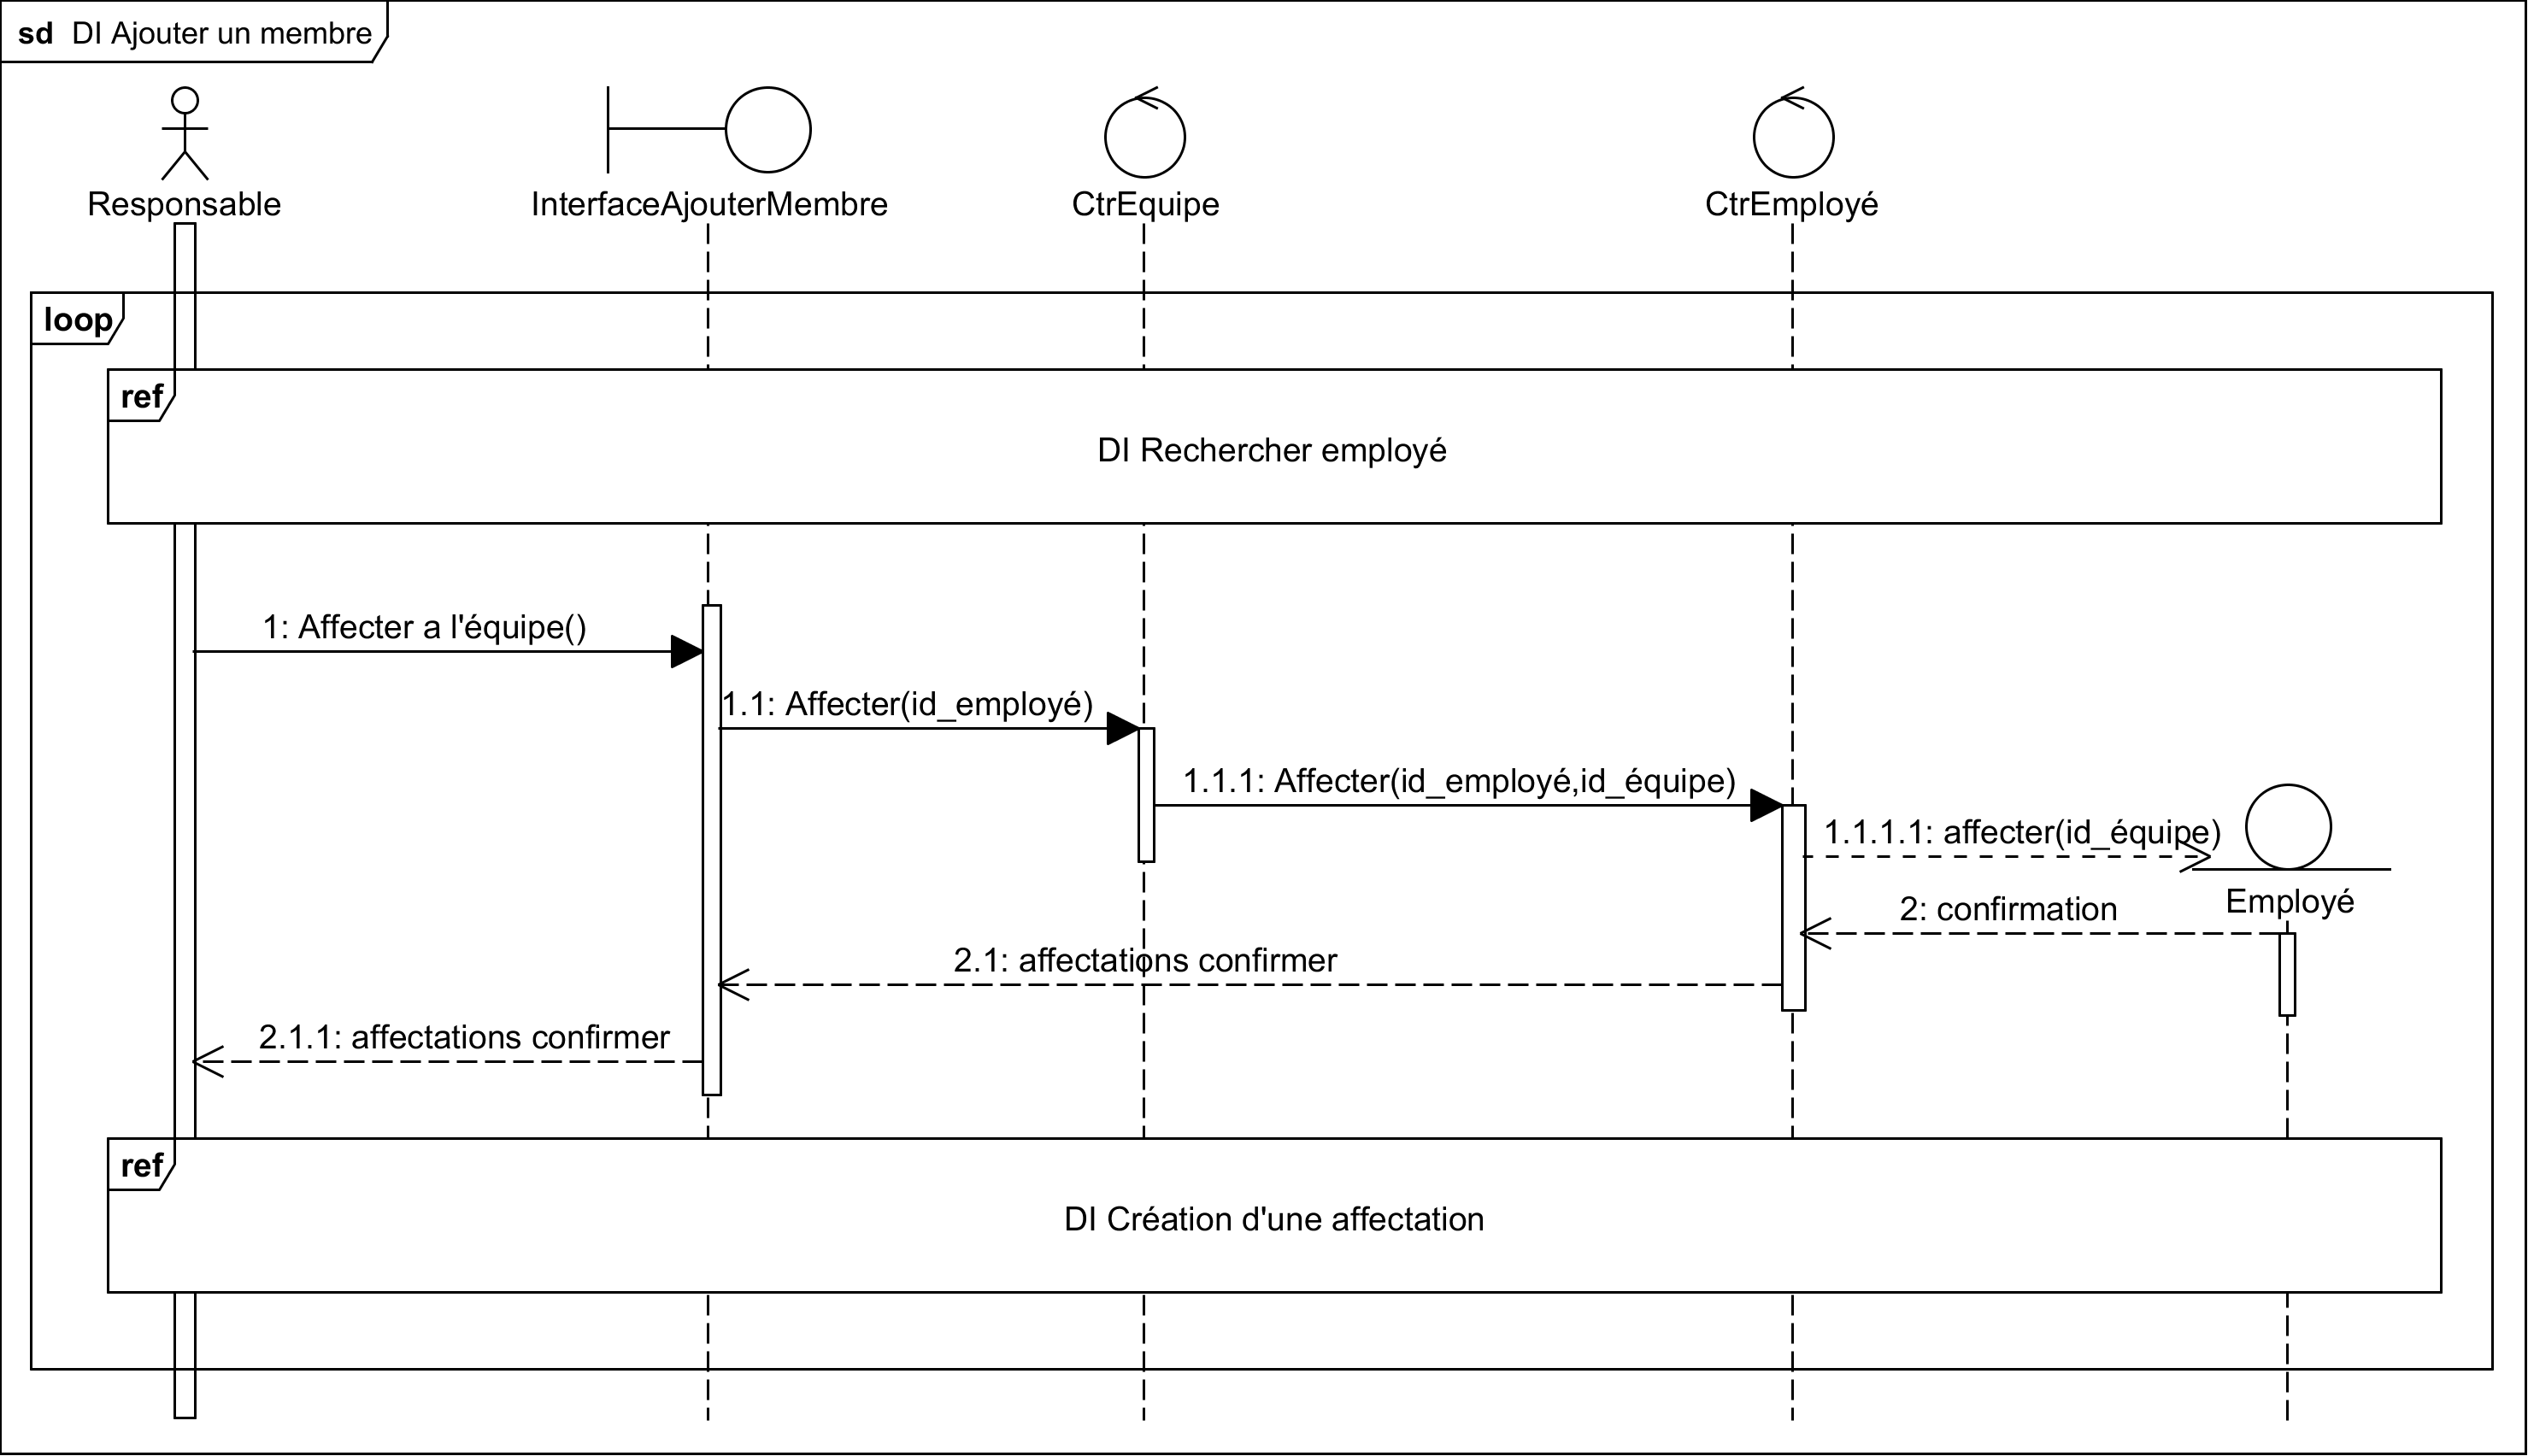
\includegraphics[ scale=0.69]{images/DS/DI Ajouter un membre.png}
    \caption{Diagramme d'interaction « Ajouter membre »}
    \label{fig40}
\end{figure}


\subsection*{Diagramme d'interaction du cas d'utilisation « Ajouter employé »}
À travers l’interface InterfaceGestionEmployé, l’administrateur aura la
possibilité d’ajouter un employé en saisissant les informations. Après la
validation, une vérification des données est effectuée avant l’ajout de
l’employé. Une fois créé, le contrôle ctrEmpreinte se chargera d’ajouter son
empreinte qui déclenchera la destruction de l’interface d’ajout et
l’administrateur sera redirigé vers l’interface InterfaceGestionEmployé avec la
nouvelle liste des employés.

\clearpage

\begin{figure}[h!]
    \centering
    \includegraphics[scale=0.7]{images/DS/DI Ajouter employé.png}
    \caption{Diagramme d'interaction « Ajouter employé »}
    \label{fig41}
\end{figure}

\subsection*{Diagramme d'interaction du cas d'utilisation « Consulter profil d'un employé »}
Une fois authentifié, le responsable aura la possibilité de consulter le profil
d’un employé. L’interface InterfaceProfileEmployé déléguera au contrôle
CtrEmployé la recherche de l’employé sélectionner, puis lui retournera les
informations concernant ce dernier. Il pourra aussi à travers cette interface
être redirigé vers l’interface de modification du profil ainsi que vers
l’interface qui lui permettra de consulter le planning de cet employé.
        
\clearpage
        
\begin{figure}[h!]
    \centering
    \includegraphics[scale=0.82]{images/DS/consulter_profil_d'un_employé.png}
    \caption{Diagramme d'interaction « Consulter profil d'un employé »}
    \label{fig42}
\end{figure}
    
\section{Diagramme de classes conception préliminaire}
En partant du modèle d’analyse, nous allons affiner et compléter les diagrammes 
de classes participantes obtenus précédemment. Pour cela, nous utiliserons les 
diagrammes de séquence que nous venons de réaliser pour:

\begin{itemize}
    \item [\textbullet] Ajouter ou préciser les opérations dans les classes 
        (un message ne peut être reçu par un objet que si sa classe a déclaré 
        l’opération publique correspondante).
    \item [\textbullet] Ajouter des types aux attributs et aux paramètres et 
        retours des opérations. 
    \item [\textbullet] Affiner les relations entre classes: associations 
        (avec indication de navigabilité), généralisations ou dépendances.\cite{5}
\end{itemize}
    
\clearpage

\subsection*{Diagramme de classes conception préliminaire du cas d'utilisation « Consulter ma fiche de pointage »}

\begin{figure}[h!]
    \centering
    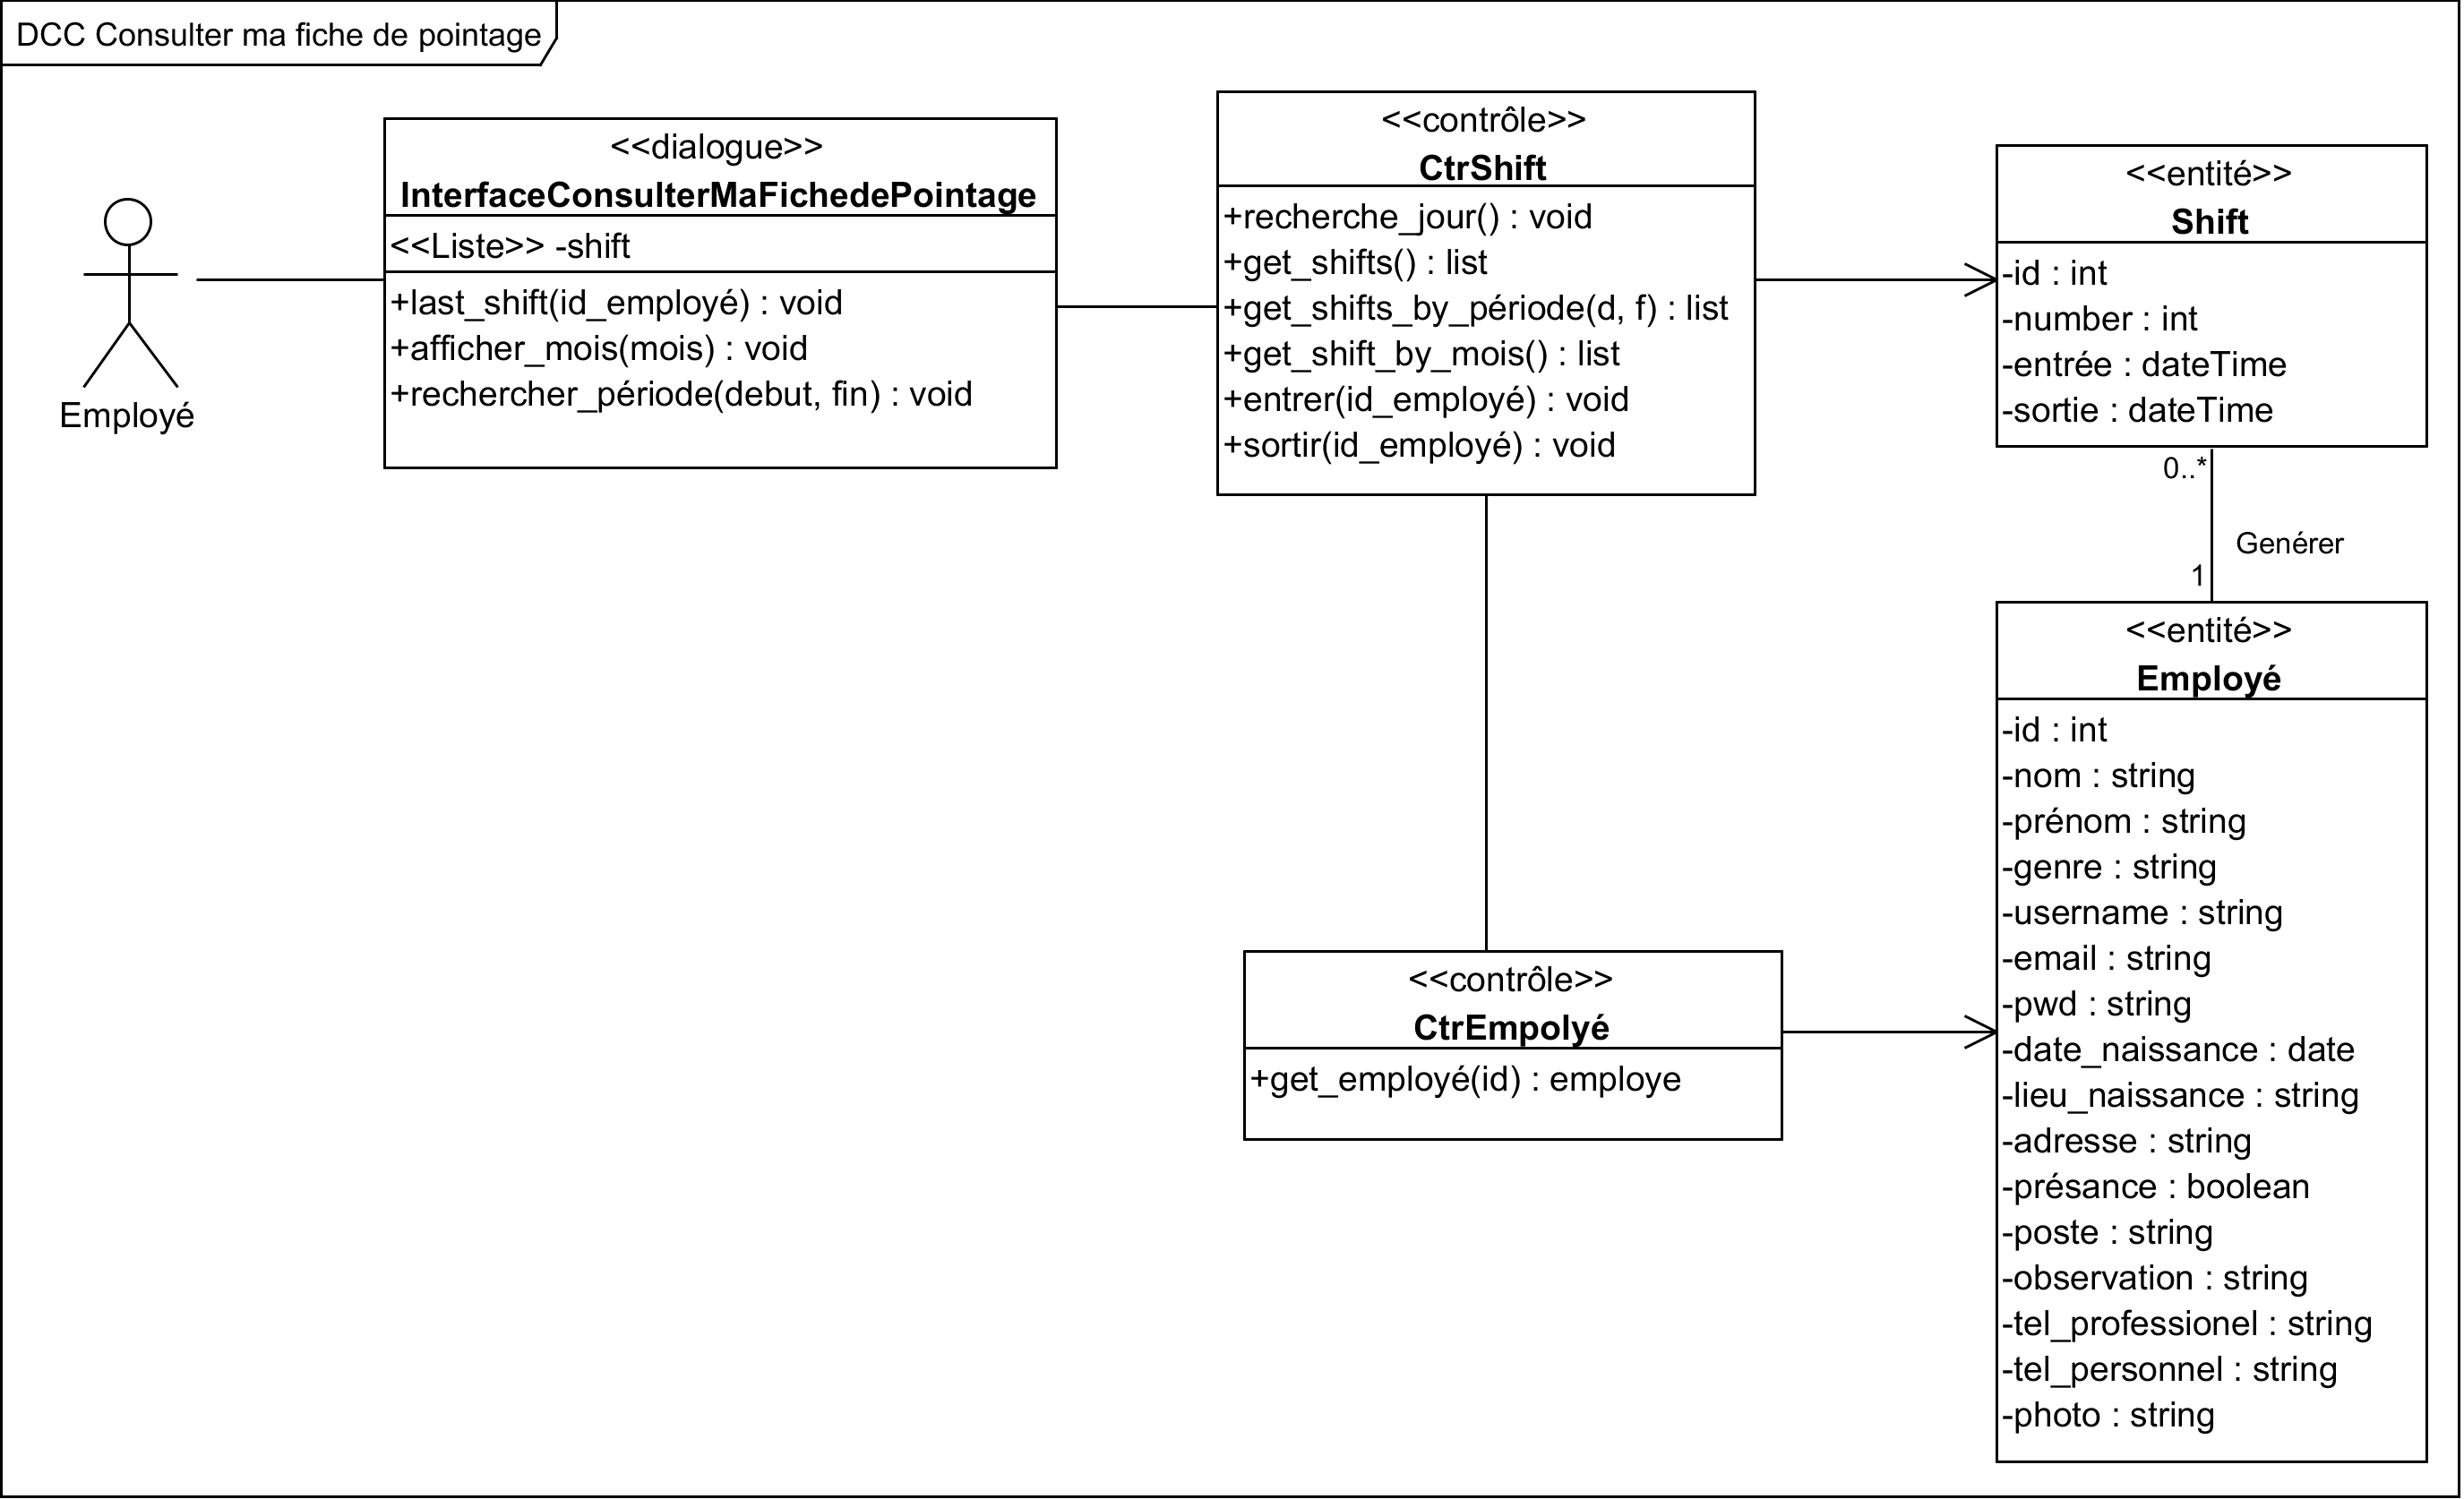
\includegraphics[scale=0.74]{images/DCC/DCC Consulter ma fiche de pointage.png}
    \caption{Diagramme de classes conception préliminaire « Consulter ma fiche de pointage »}
    \label{fig42}
\end{figure}
        
\subsection*{Diagramme de classes conception préliminaire du cas d'utilisation « Ajouter une équipe »}

\clearpage

\begin{figure}[h!]
    \centering
    \includegraphics[scale=0.7]{images/DCC/DCC Ajouter une équipe.png}
    \caption{Diagramme de classes conception préliminaire « Ajouter une équipe »}
    \label{fig43}
\end{figure}
        
\subsection*{Diagramme de classes conception préliminaire du cas d'utilisation « Ajouter un planning »}

\begin{figure}[h!]
    \centering
    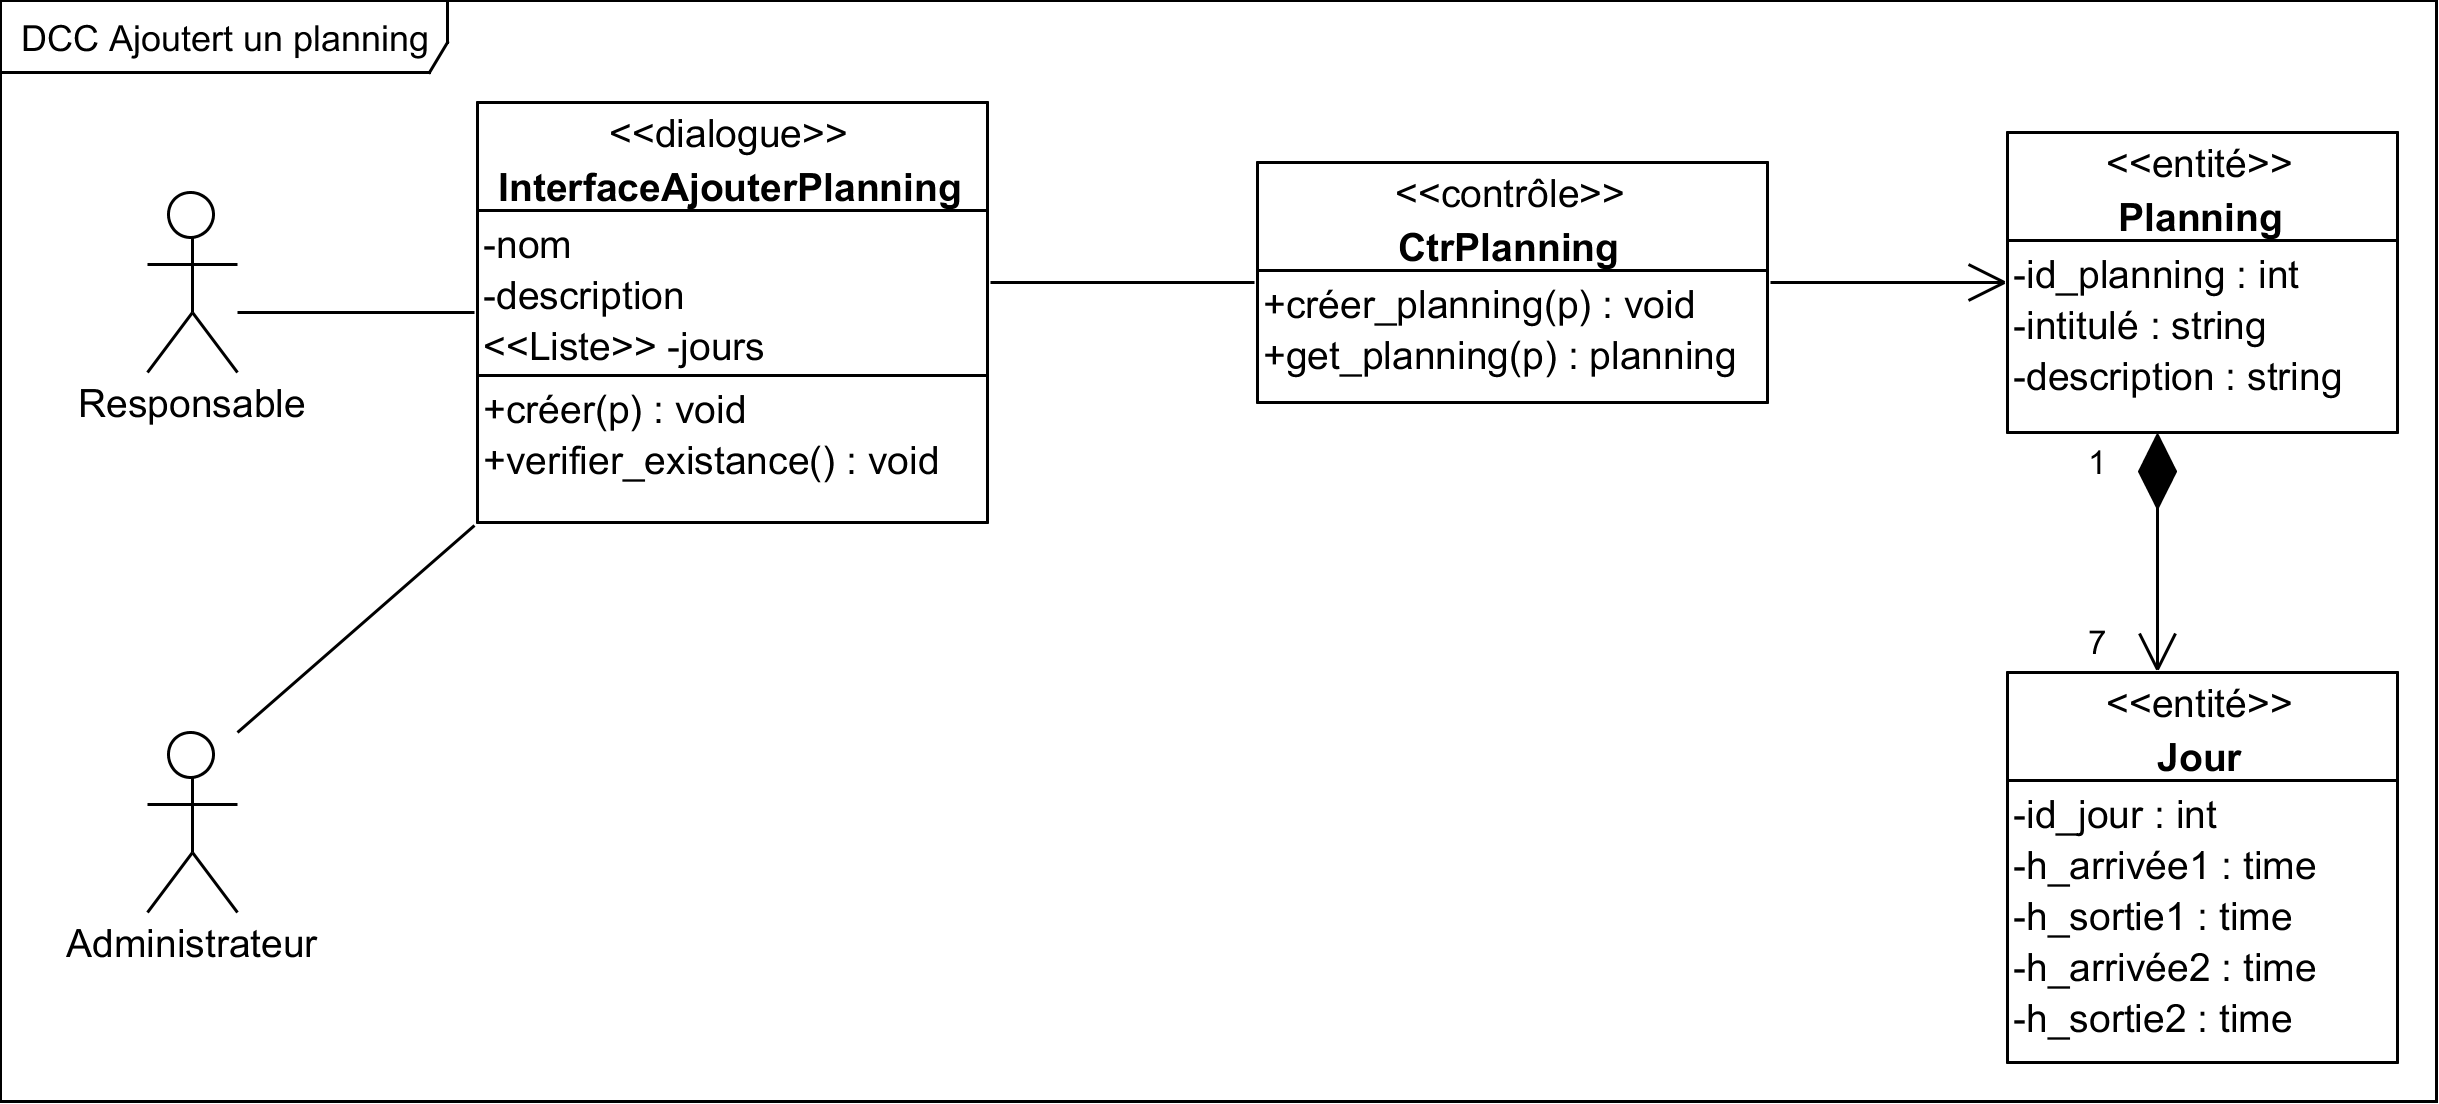
\includegraphics[scale=0.7]{images/DCC/DCC Ajoutert un planning.png}
    \caption{Diagramme de classes conception préliminaire « Ajouter un planning»}
    \label{fig44}
\end{figure}
        
\clearpage

\subsection*{Diagramme de classes conception préliminaire du cas d'utilisation « Ajouter un employé »}

\begin{figure}[h!]
    \centering
    \includegraphics[scale=0.7]{images/DCC/DCC Ajouter employé.png}
    \caption{Diagramme de classes conception préliminaire « Ajouter un employé»}
    \label{fig45}
\end{figure}

\subsection*{Diagramme de classes conception préliminaire du cas d'utilisation « Consulter profil d'un employé »}

\begin{figure}[h!]
    \centering
    \includegraphics[scale=0.74]{images/DCC/DCC Consulter profil d'un employé.png}
    \caption{Diagramme de classes conception préliminaire « Consulter profil d'un employé»}
    \label{fig46}
\end{figure}

\section{Diagramme de classe conception}
Les diagrammes de classes décrivent la structure ou plutôt l’architecture d’un
système et sont donc la base de presque toutes les autres techniques de
description. En conséquence, les diagrammes de classes, et en particulier les
classes, sont un concept qui est utilisé universellement en modélisation et en
programmation. Ils permettent l’encapsulation des attributs et des méthodes et
la représentation des instances sous forme d’objets\cite{10}.

À l’aide des diagrammes de classe de conception établis dans la section
précédente, nous avons modélisé le diagramme de classe ci-dessous.

\begin{figure}[h!]
    \centering
    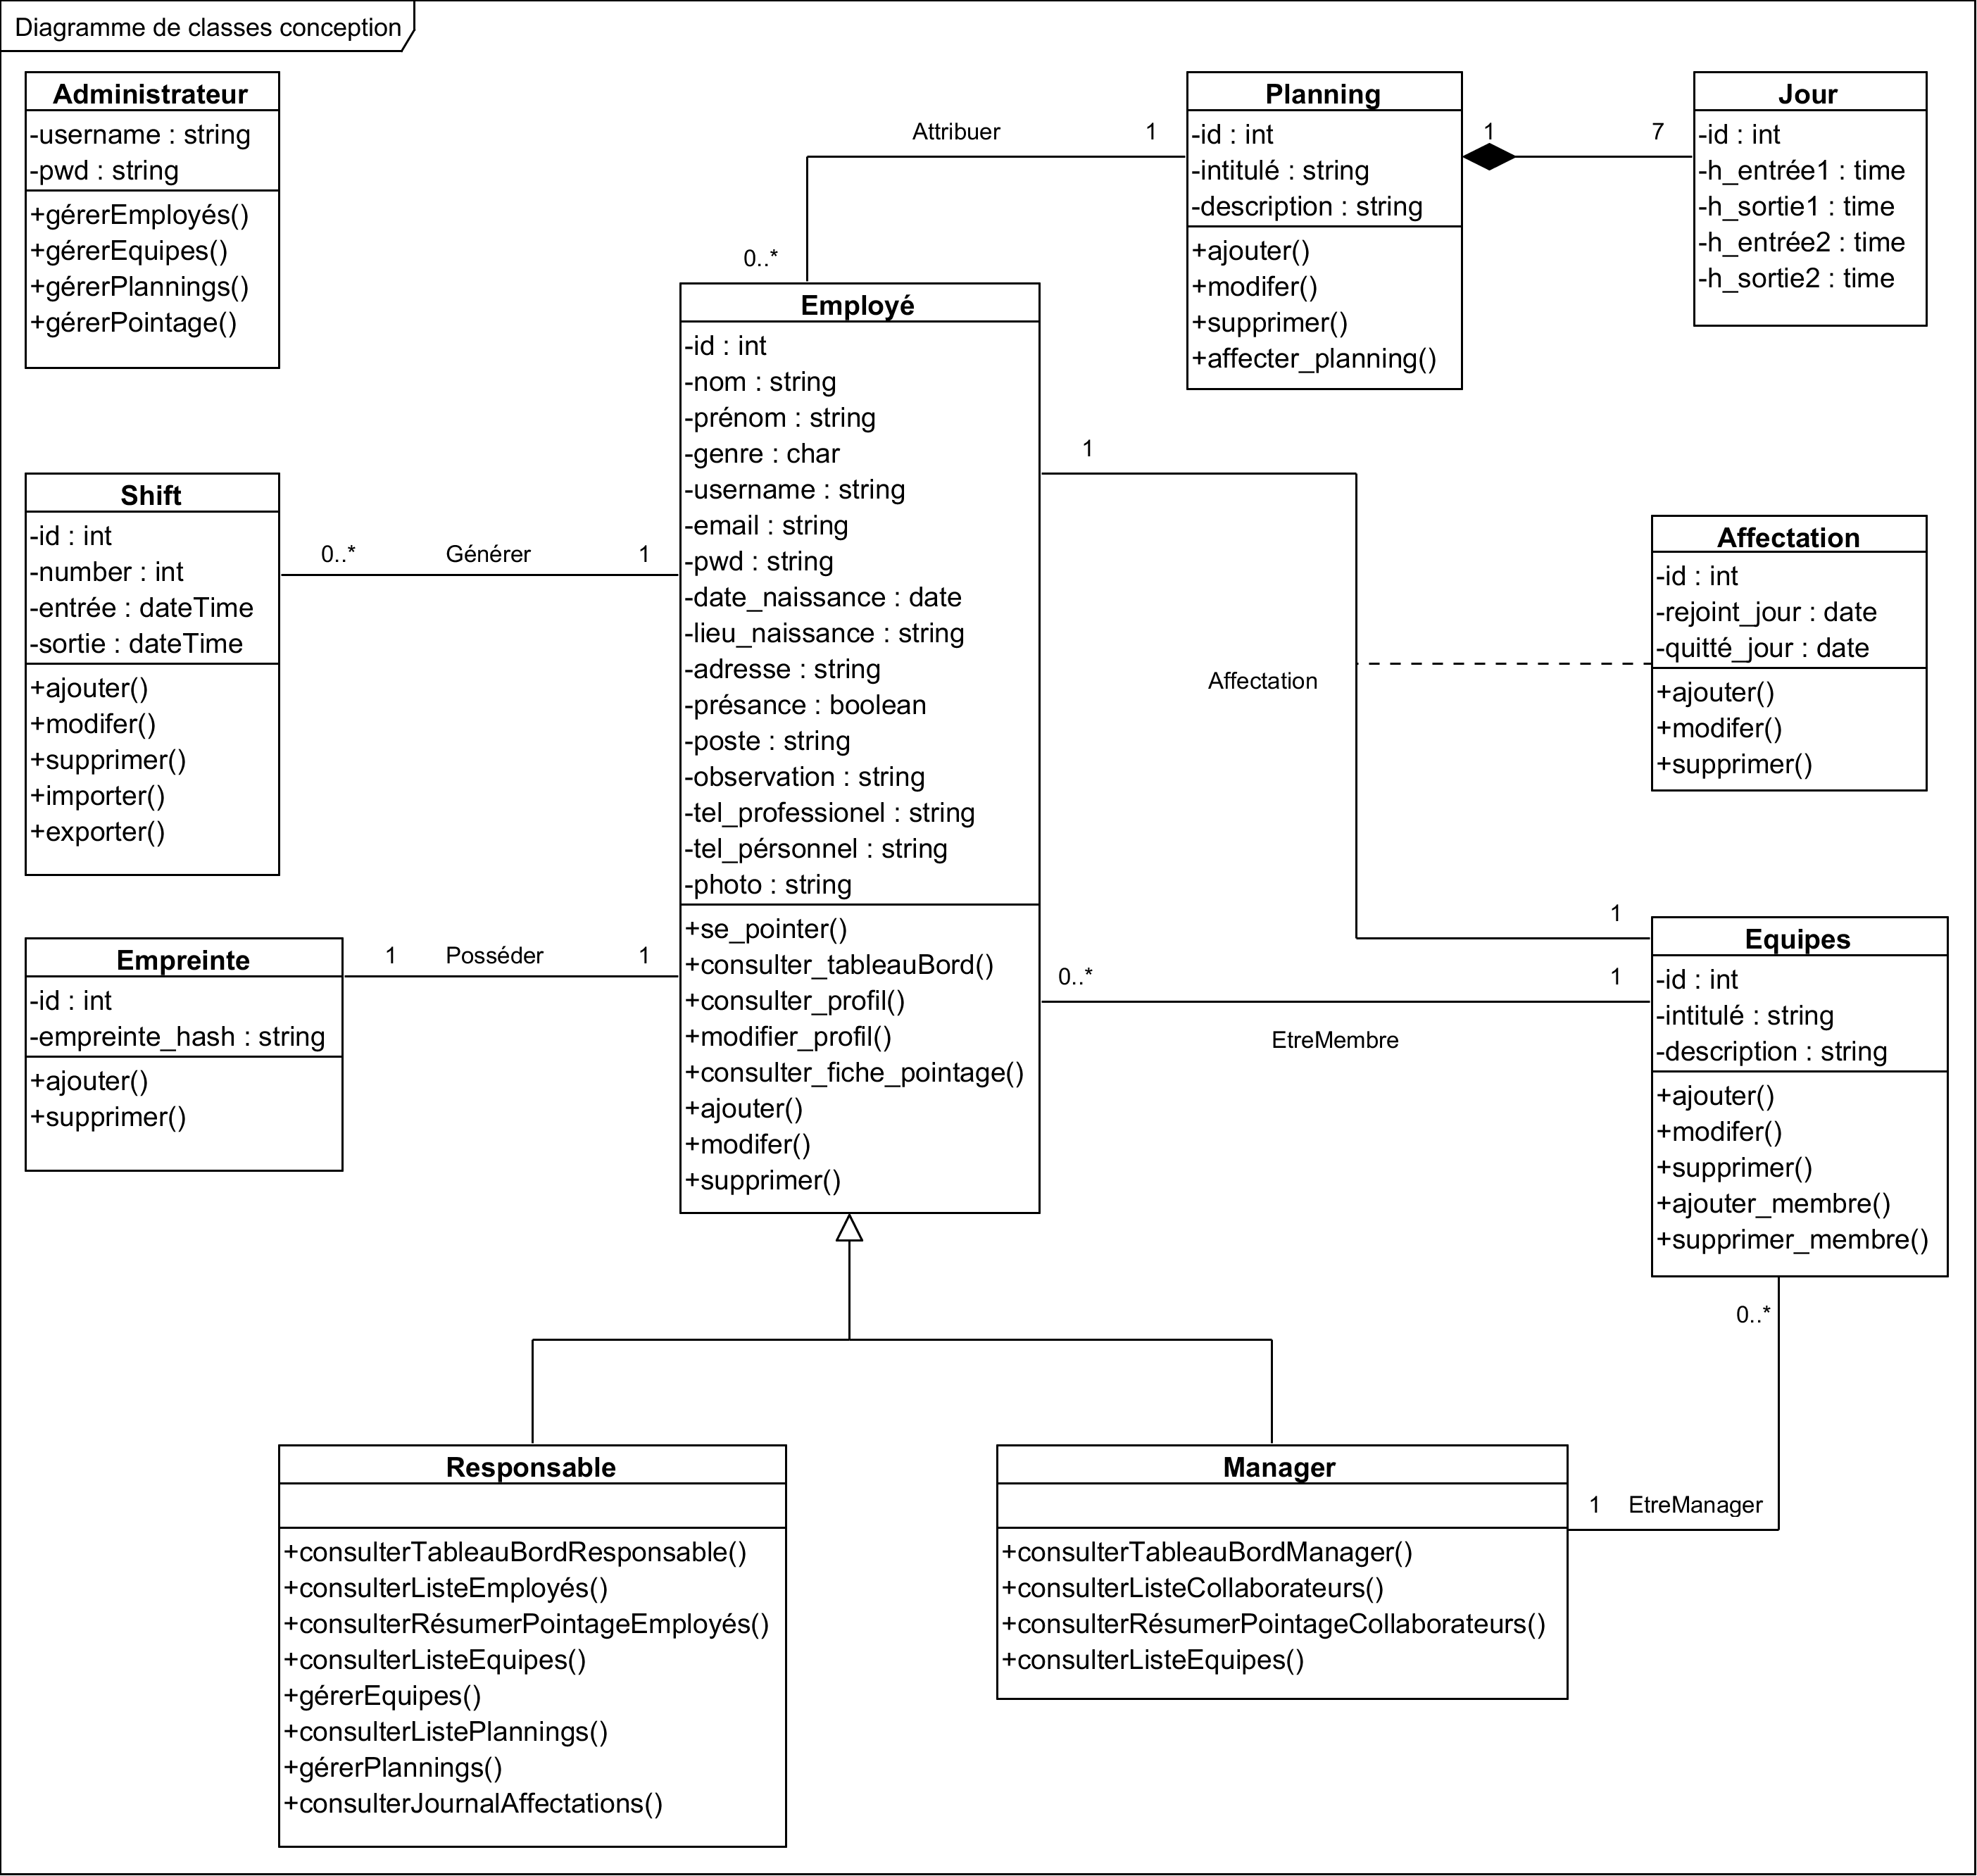
\includegraphics[scale=0.69]{images/DCC/Diagramme de classe.png}
    \caption{Diagramme de classe}
    \label{fig47}
\end{figure}

\section{Modèle relationnel}
Le modèle relationnel a vu le jour en 1970 avec les travaux de Edgar Frank 
Codd. La principale publication est « A Relational Model for Large Shared Data 
Banks », Communications of the ACM, vol. 13, n° 6, 1970.\\

\begin{figure}[h!]
    \centering
    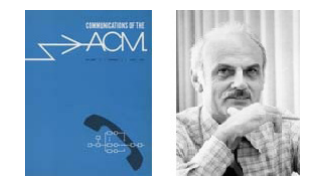
\includegraphics[scale=1]{images/pere_mr.PNG}
    \caption{Le père du modèle relationnel}
    \label{fig48}
\end{figure}
        
Ce modèle de données est construit principalement autour des concepts suivants \cite{11}:

\begin{itemize}
    \item[\textbullet] Relation: structure de données qui préfigure la table qui 
        sera créée à l’aide du langage SQL.
    \item[\textbullet]  Attribut: représentation d’une information atomique qui 
        préfigure une colonne d’une table. Un domaine de valeurs devrait être défini 
        ainsi que d’éventuelles règles de validation (contraintes).
    \item[\textbullet] Clé primaire: attribut(s) identifiant une relation qui 
        préfigure(nt) la primary Key de la table.
    \item[\textbullet] Clé étrangère: attribut(s) qui référence(nt) une tierce 
        relation, préfigure(nt) une foreign Key de la table.             
\end{itemize}

Afin de pouvoir implémenter une base de données, il faut pouvoir traduire le 
modèle conceptuel en modèle logique. Cela signifie qu’il faut pouvoir convertir 
un modèle UML en modèle relationnel. Les modèles conceptuels sont suffisamment 
formels pour que ce passage soit systématisé dans la plupart des cas. 
En appliquant les règles de passage\cite{12}, nous obtenons les relations suivantes:

\begin{itemize}
    \item [\textbullet]\textbf{Employé}(\underline{id\_employé}, nom, prénom, genre, 
        username, email,pwd, date\_naissance,lieu-naissance, adresse, présence, poste, 
        observations, tél\_professionnel, tél\_personnel, photo, type,\#ggid\_équipe, 
        \#ggid\_planning, \#id\_empreinte).

	\item [\textbullet]\textbf{Planning}(\underline{id\_planning}, intitulé, 
        description).
    
    \item [\textbullet]\textbf{Jour}(\underline{id\_jour}, h\_entrée1, h\_sortie1, 
        h\_entrée2, h\_sortie2, \#ggid\_planning).
    
    \item [\textbullet]\textbf{Équipe}(\underline{id\_équipe}, intitulé, 
        description, \#ggid\_employé).
    
    \item [\textbullet]\textbf{Affectation}(\underline{id\_affectation}, 
        rejoint\_jour, quitté\_jour, \#ggid\_équipe, \#id\_employé).
    
    \item [\textbullet]\textbf{Shift}(\underline{id\_shift},num\_séquence, 
        h\_entrée, h\_sortien, \#ggid\_employé ).
    
    \item [\textbullet]\textbf{Empreinte}(\underline{id\_empreinte}, 
        empreinte\_hash)
    
    \item [\textbullet]\textbf{Administrateur}(\underline{id\_administrateur}, 
        username, email, pwd).
\end{itemize}

\section{Conclusion}
Au cours de ce chapitre, nous avons en premier lieu identifié les modèles du
domaine pour avoir une vue globale sur les différentes entités de notre système,
puis nous avons modélisé les diagrammes de classes participantes et
d’interactions qui permettent l’enrichissement des diagrammes de séquences
système. Par la suite, en modélisant les diagrammes de classe conception
préliminaire, nous avons pu établir le diagramme de classe conception.  Enfin,
pour avoir une vue plus structurée et implémenter une base de données nous avons
traduit ce dernier diagramme en un modèle relationnel. 
